\chapter{Deformation studies of a ladder under the test beam}
\label{chap:deformation}

  The first full-scale prototype which embeds twelve sensors glued on a copper flex-cable and a 8 \% density \gls{SiC} foam was tested in November 2011 at CERN-SPS facility with a pions beam of 120 GeV.
  The motivations to perform such a test in real conditions are first, to make sure that the ladder is working properly.
  Secondly, to verify the response homogeneity of each sensor.
  Finally, it has to prove the benefits of a double sided measurement.
  This chapter does not aim to present fully the test beam campaign and all the results but to focus on a specific study of the ladder's deformation observed during the alignment procedure.
  More results about this test beam are presented in Loic \textsc{Cousin}'s thesis \cite{cousin}.
  This chapter will present the test beam facility, as well as the experimental set-up.
  The alignment procedure is explained and some results for the ladder positioned in a normal incidence, as well as the ladder tilted in one direction, are discussed.
  The second part of the chapter will focus on the deviation observed during the alignment and will discuss a method to overcome these deformations.
  Finally, the benefits of double-sided measurements will be introduced.
  
  \minitoc

  \section{Test beam of the full complete PLUME ladder at CERN}

    \subsection{Test beam facility and beam test set-up}

    The test beam was performed at CERN-SPS in the North hall on the H6 beam line.
    Negative pions with an energy of 120 GeV were used.
    The spill structure was 9.6 s with a dead time of 45.6 s. 
    The bench set-up is composed of a telescope equipped with four standard MIMOSA-26 sensors, thinned down to 120 $\mu\text{m}$ and used as reference planes.
    It is made of two arms and the distance between two sensors of the same arm is 5 mm.
    The reference planes are stabilised to a temperature of 15 degrees Celsius and a 8 sigma S/N threshold cut was applied.
    The \gls{PLUME} ladder is positioned between the two telescope arms for the tests.
    For the rest of the chapter, the ladder is called the \gls{DUT}.
    The bench has also $7 \times 7$ scintillators used for triggering the data.
    Most of the runs were taken with a trigger frequency between 2 and 8 kHz, except for two days where the frequency was oscillating between 1 and 1.3 kHz.
    The acquisition system is limited to eight inputs and four of them are used by the telescope.
    Thus, only four sensors of the \gls{DUT} were connected to the acquisition, two on each side.
    The temperature of the \gls{DUT} was stabilised thanks to an air flow cooling system, provided by a fan.

    \subsection{Cartesian coordinate systems}

    Although the sensors have their own ID to distinguish them during the analysis, the position of each plane has to be known exactly.
    Two Cartesian coordinate systems are then defined.
    The first one is the global one and is determined by the position of each sensor of the telescope.
    The notation used for this coordinate system is $(x,y,z)$.
    The $x$-axis corresponds to the horizontal direction, the $y$-axis is the vertical one and the $z$-axis is along the beam direction.
    The origin $(0,0,0)$ of the system is usually defined by the position of the first plane hit.
    The second coordinate system is the local one and is determined by a single sensor.
    To differentiate this reference system to the other one, the $(u,v,w)$  notation is used.
    The $u$-axis corresponds to the pixel rows, the $v$-axis is along the pixel columns and the $w$-axis is perpendicular to the matrix.
    The origin of the local system is the center of the pixel matrix.
    Figure~\ref{fig:labCoordinates} summarises the definition of the two coordinate systems.\todo{Draw a better figure}

    \begin{figure}[!h]
      \centering
      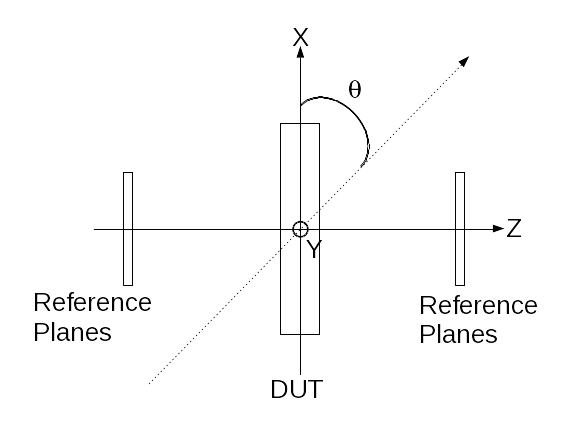
\includegraphics[width = 0.7\textwidth]{Pictures/deformation/lab_frame.png}
      \caption{Drawing of the laboratory coordinates.}
      \label{fig:labCoordinates}
    \end{figure}

    \subsection{Measurements}

    The prototype validation was done under several conditions.
    Firstly, three different geometric configurations were used.
    On the first one presented on figure~\ref{fig:tbNormal}, the \gls{DUT} is parallel to the telescope planes and the beam is hitting the device in a normal incidence.
    The ladder is placed in between the two arms.
    The middle of the foam is at equal distance from both inner telescope planes.
    For the second configuration, as shown on figure~\ref{fig:tilt36}, the distance between the telescope planes are the same, but the \gls{DUT} is tilted between 28 and 40 degrees along the $y$-axis.
    Runs with a larger angle (60 degrees) were done.
    Due to the PLUME box's size, the cabling for the acquisition, the air cooling system and the design of the telescope stage, limiting the spacing between the two arms, the \gls{DUT} was placed behind the two arms, as presented on figure~\ref{fig:tilt60}.
    For both configurations, different parameters were modified.
    The thresholds were set to 5 and 6 mV, different sensors were aimed and the air flow speed was set to 3 $\text{m.s}^{-1}$ and 6 $\text{m.s}^{-1}$.

    \begin{figure}[!h]
      \centering
      \begin{subfigure}[t]{0.9\textwidth}
        \centering
        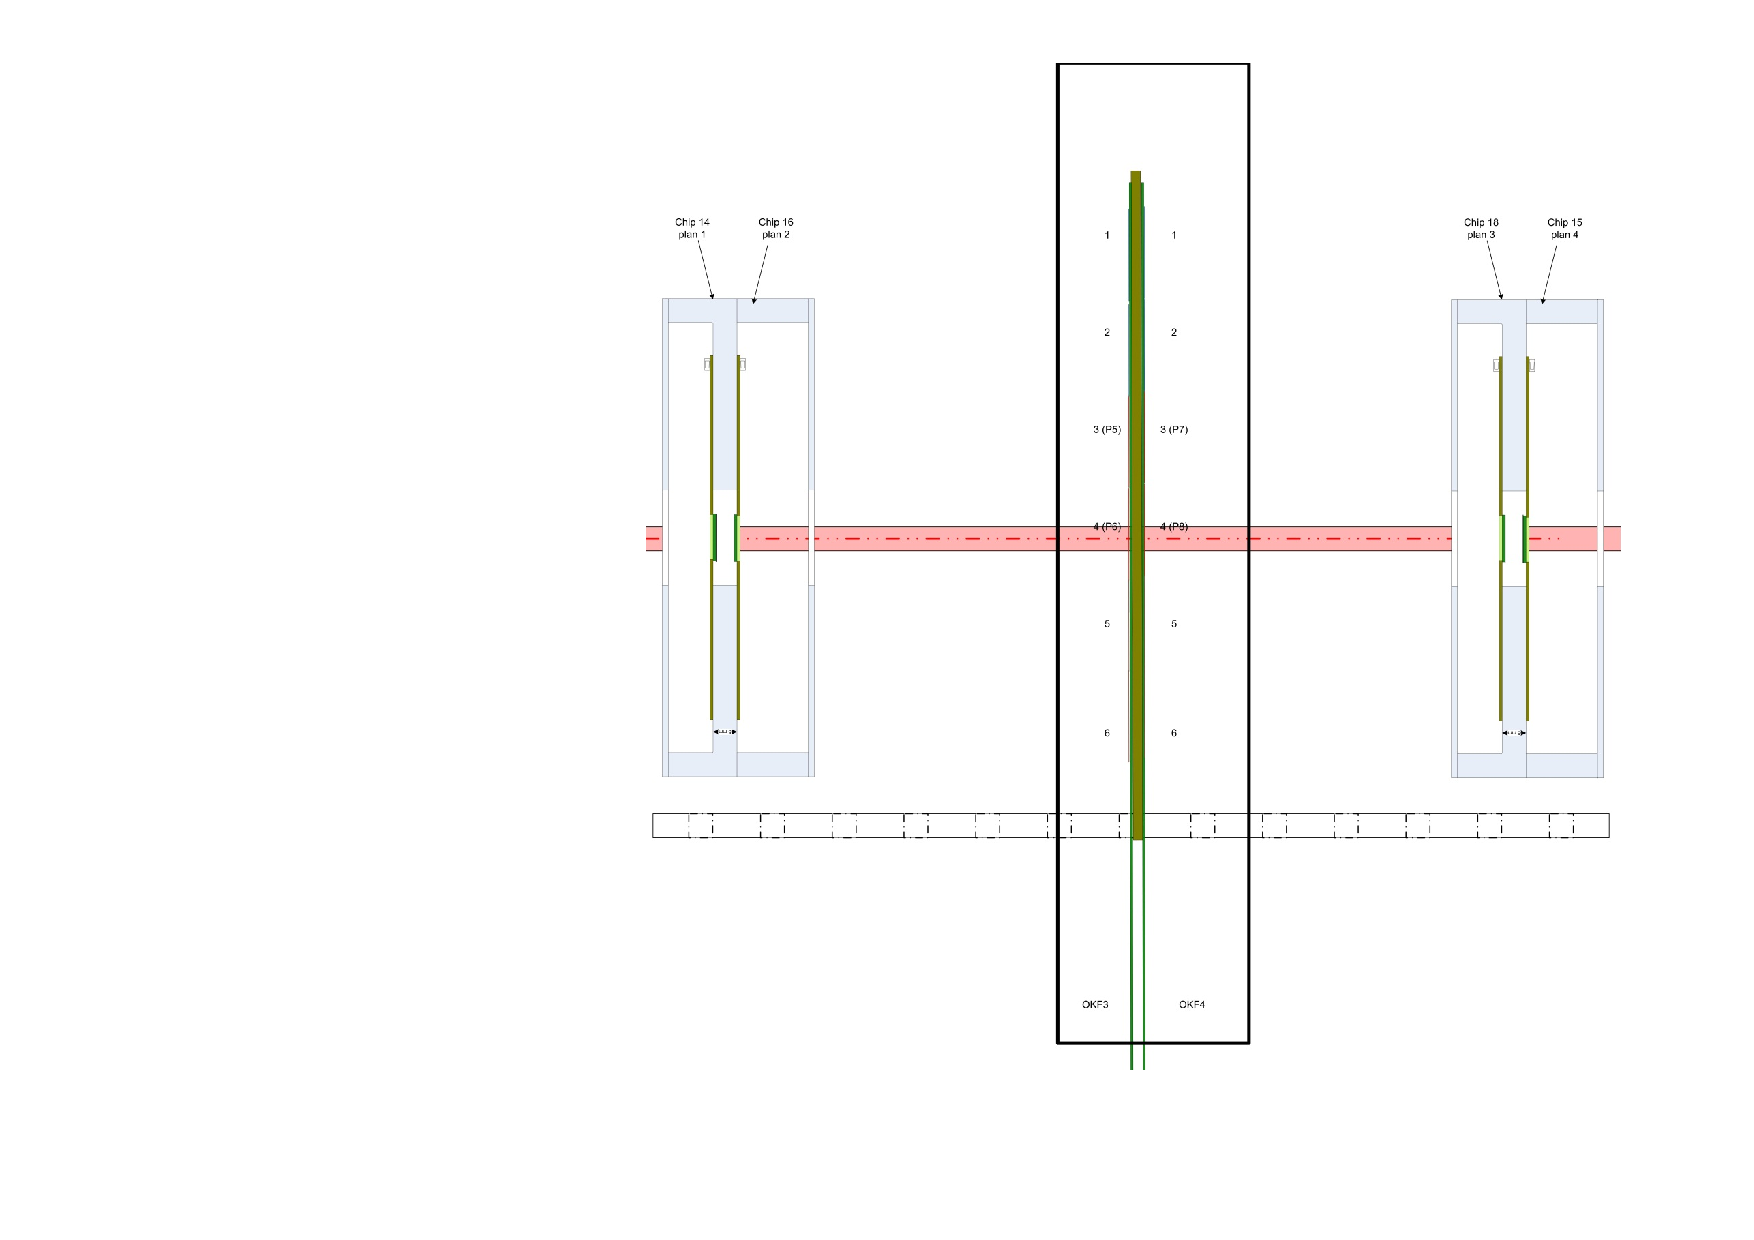
\includegraphics[width = 0.5 \textwidth]{Pictures/deformation/tb_cern_11_sketch_normal.pdf}
        \caption{Configuration for normal incidence with respect to the beam direction.}
        \label{fig:tbNormal}
      \end{subfigure}

      \begin{subfigure}[t]{0.45\textwidth}
        \centering
        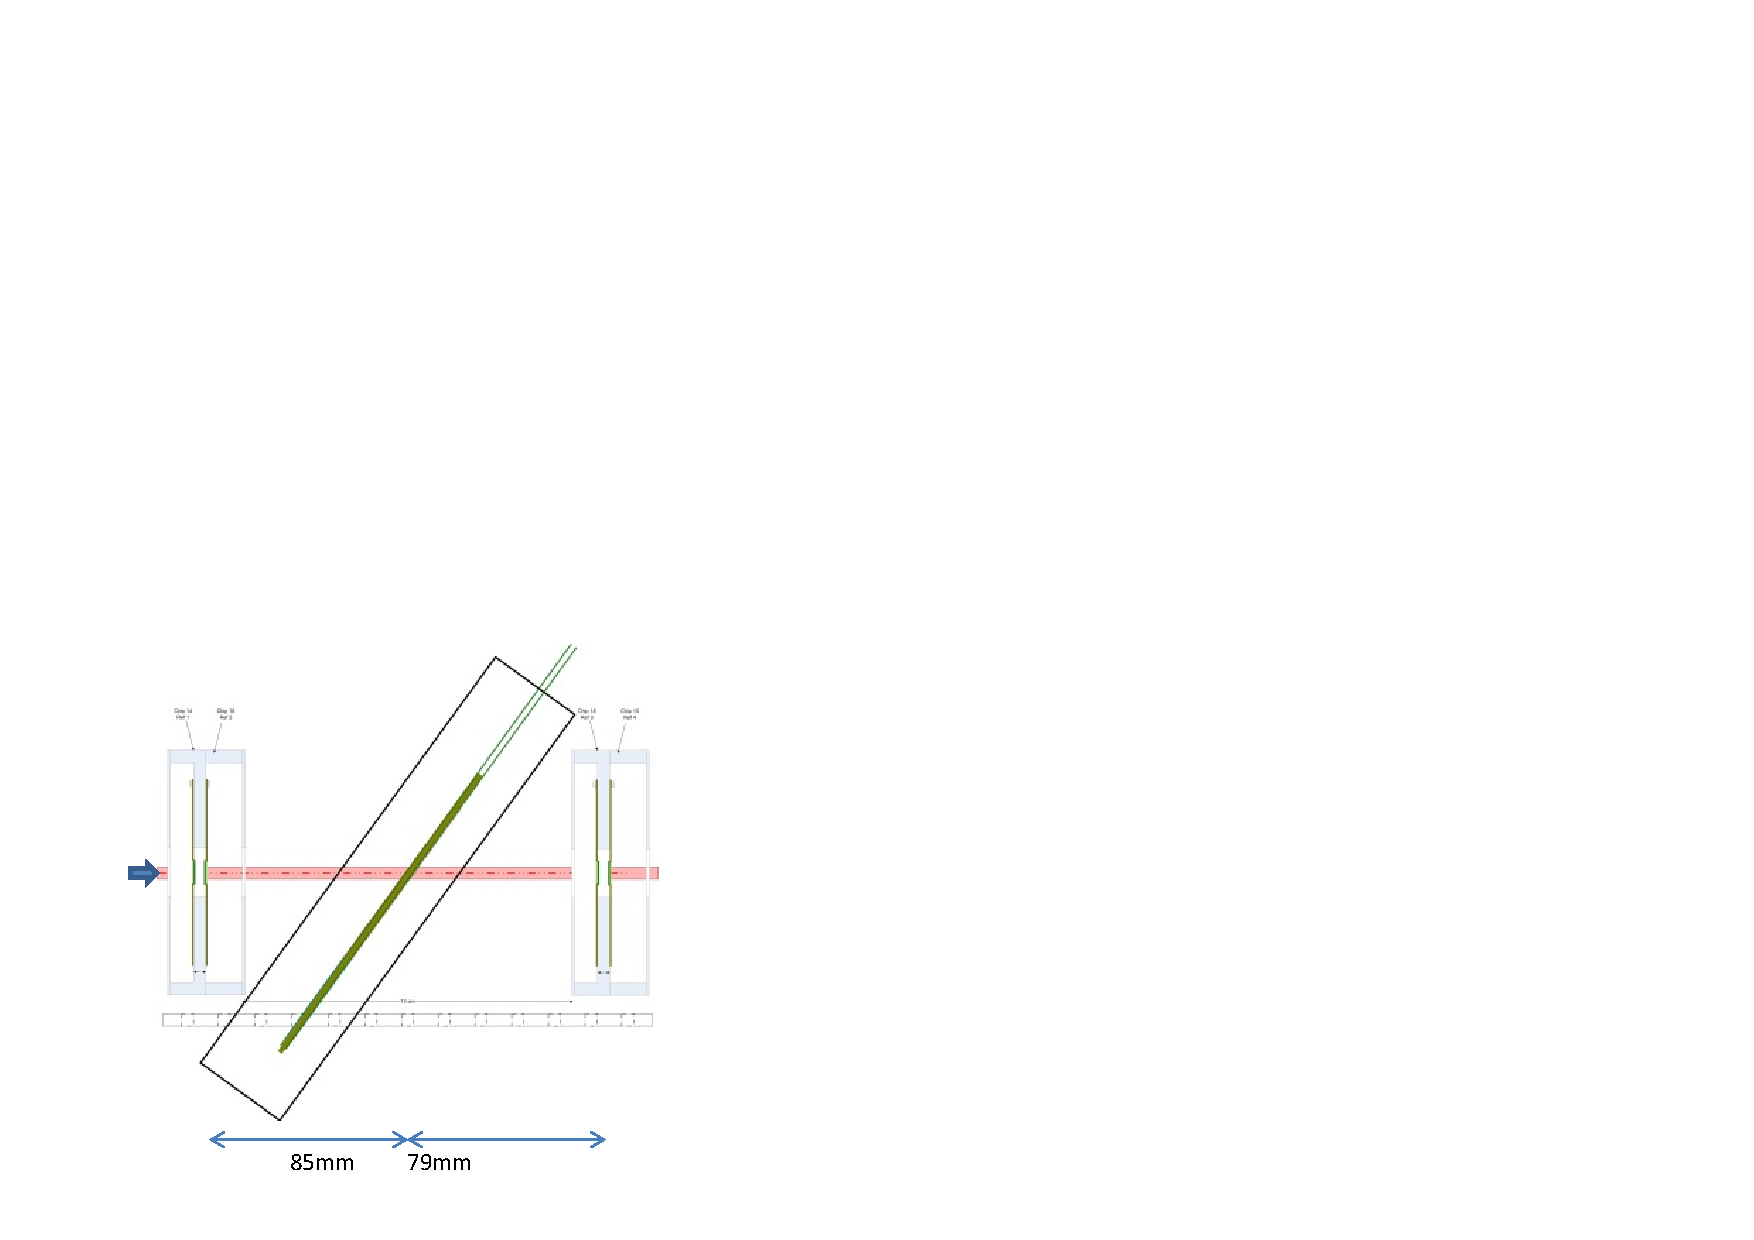
\includegraphics[width=0.8\textwidth]{Pictures/deformation/tb_cern_11_sketch_tilted.pdf}
        \caption{Configuration for an angle between 28 and 40 degrees.}
        \label{fig:tilt36}
      \end{subfigure}
      ~%\quad
       %add desired spacing between images, e. g. ~, \quad, \qquad, \hfill etc. 
        %(or a blank line to force the subfigure onto a new line)
      \begin{subfigure}[t]{0.45\textwidth}
        \centering
        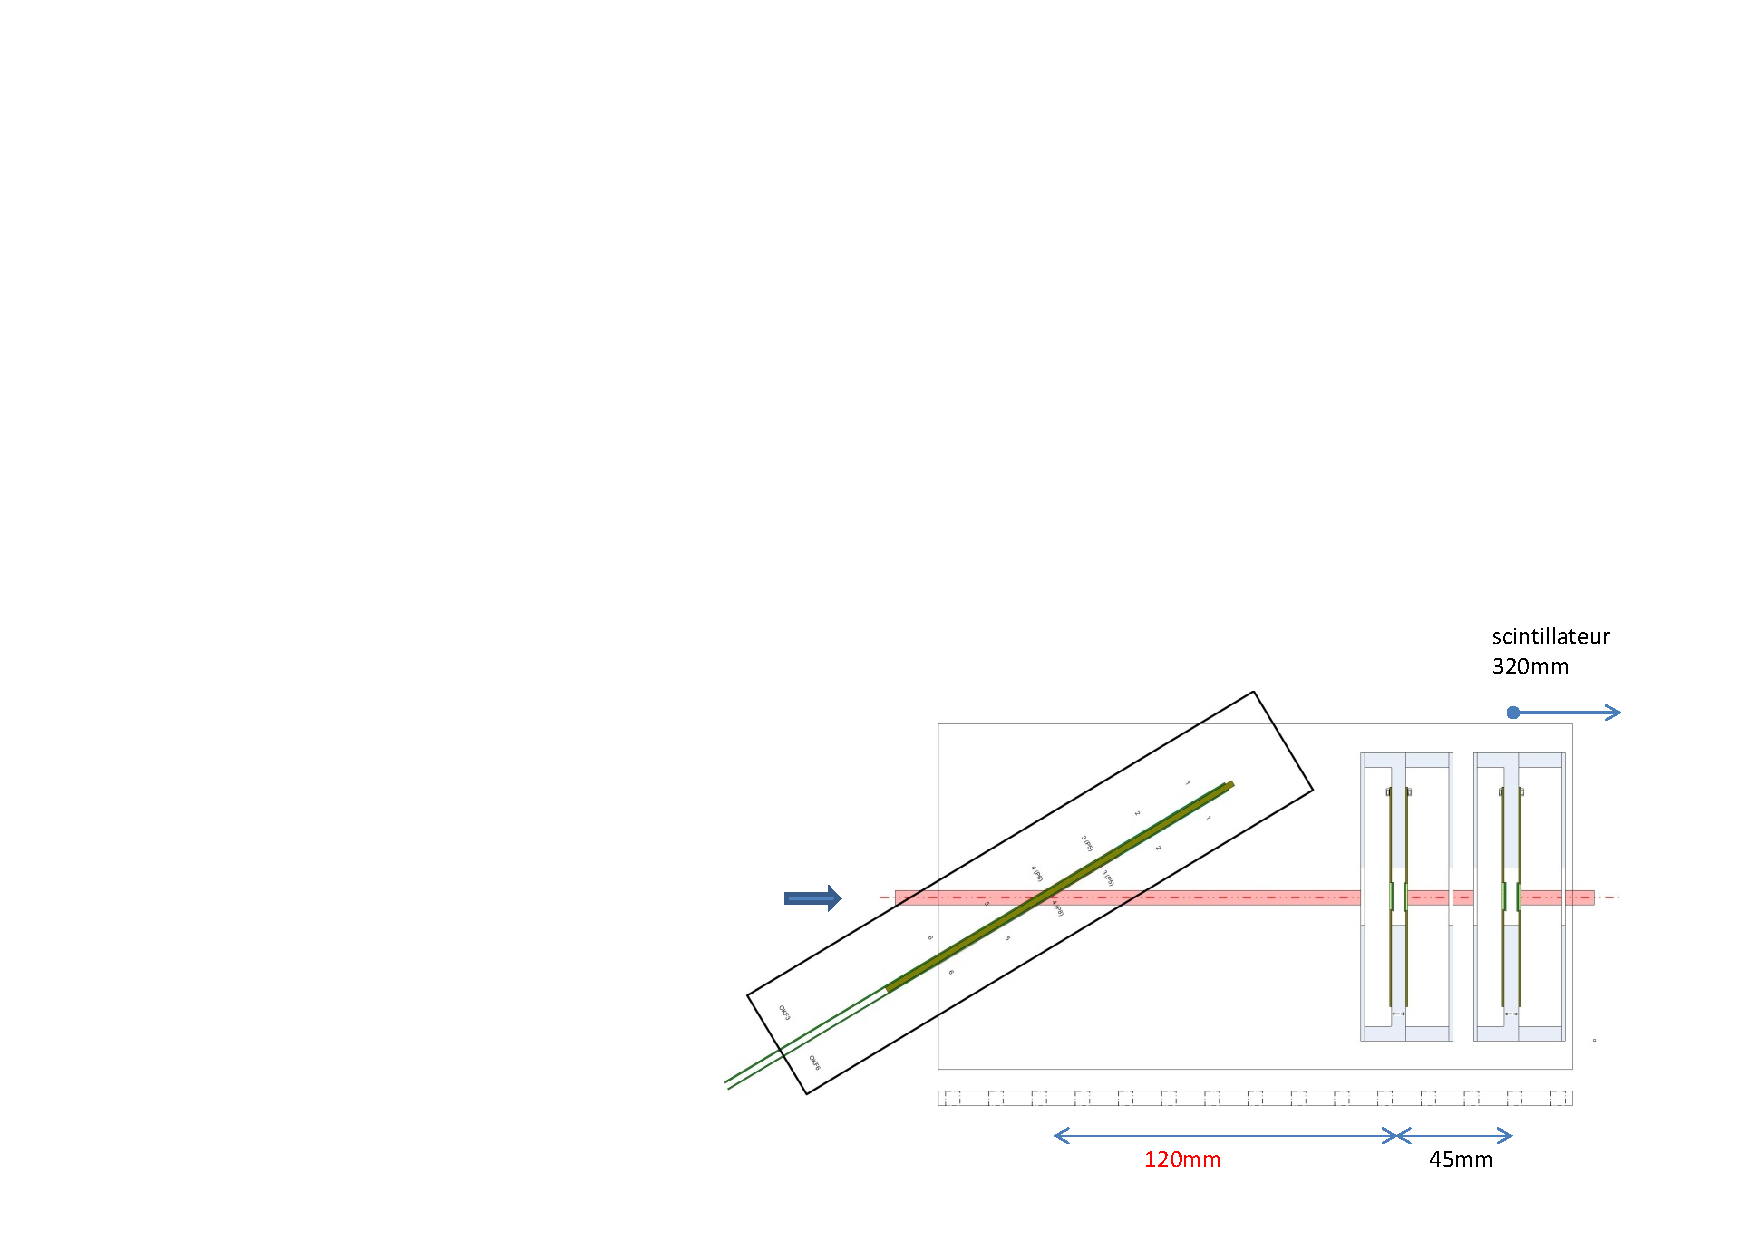
\includegraphics[width=0.95\textwidth]{Pictures/deformation/tb_cern_11_sketch_tilted120mm.pdf}
        \caption{Configuration for an angle of 60 degrees.}
        \label{fig:tilt60}
      \end{subfigure}
      \caption{Top view sketches of the test beam configuration for different ladder positions: \ref{fig:tbNormal} is for normal incidence, \ref{fig:tilt36} and \ref{fig:tilt60} are for tilted ladder.}
      \label{fig:tilt}
    \end{figure}   

    The analysis and the results shown in the following sections were performed with \gls{TAF}, the analysis software developed by the IPHC and presented in chapter~\ref{chap:labTests}.

  \section{Spatial resolution studies}
   
    One of the measurements performed during the analysis is to determine the pointing resolution of the ladder.
    As the sensors used are well-known, the performance of the ladder should be similar to the one expected.
    Any deviations on the pointing resolution or the efficiency might point out an unexpected impact of the mechanical structure or the flex-cable design over the whole system.
    The alignment steps to obtained the pointing resolution of the ladders are explained below for different run configurations. 

    \subsection{Normal incidence track}
     
    For each event, the acquisition is recording the position of the pixels hit, the frame number, as well as the sensor ID.
    %The sensors are sending to the acquisition the position of the pixel hit, on which frame this event was recorded, as well as the sensor ID.
    The binary file created contains no information about the relative position of each sensor.
    To perform an analysis, the telescope planes have to be aligned each other.
    The hits information of every plane is combined in order to create tracks. 
    A track corresponds to the path of a particle through the system.
    Thanks to this information, the tracks are then compared to the hits position on the \gls{DUT} to give some information, such as the detection efficiency (the ratio of tracks matched to the hits on the \gls{DUT}) or the spatial resolution (minimum distance to distinguish two incoming tracks).

    The alignment procedure is done in two steps: firstly the telescope planes are aligned to minimise the mismatch of particles' tracks and to improve the tracking resolution.
    Afterward, the \gls{DUT} is aligned with respect to the information provided by the reference planes and then, the analysis itself is performed.
    Although the position of each sensor is measured during the test beam with a precision of the millimeter, for the analysis, a precision of the micron level has to be achieved.
    Three degrees of freedom were taken into account for the alignment here: two translations for the $x$ and $y$-axes and one rotation around the $z$-axis.
    The $z$ position is determined by the position measured during the test beam campaign and is not considered as a free parameter due to the beam used.

      \subsubsection{Alignment procedure and telescope alignment}

      Firstly, the data acquired during the test beam are processed to extract the signal and the hit information.
      For each frame, the position of the pixel(s) having a signal above the discriminator threshold is stored and assigned to an ID corresponding to a sensor.
      The analysis software is in charge to assign correctly the hit to the sensors and then to group the pixel fired into clusters.
      As the sensors used during the test beam have a binary output, no information on the seed pixel is available.
      Thus, the hit position is obtained from a centre-of-gravity calculation.

      Secondly, with the analysis software, one plane is considered as the origin of the telescope coordinate system and is used as a reference for the alignment.
      Usually, the first sensor hit by the beam is the main reference.
      The alignment means to correct the offset for the view angles and the hit position of the telescope planes and the \gls{DUT}.
      These offsets are found thanks to scattering plots where the residuals are represented as a function of predicted hit position.
      An alignment is considered as a good one when the residuals are not correlated to the predicted hit position.
      If it is not centered around zero, an offset has to be applied in this direction, whereas a slope indicates that a tilt has to be applied.
      First off, the hit positions of the first plane are extrapolated to the next planes in order to perform the alignment.
      These tracks extrapolated are straight lines perpendicular to the hits position.
      Thus, the hit position of the last telescope plane is adjusted to match the hit position of the first plane.
      The alignment is an iterative procedure which consists to minimise the residual. 
      It corresponds to the distance between the extrapolated track to the closest hit on the sensor.
      Afterward, the track candidates are built by matching a hit on the first plane to a hit on the last one.
      The second and third telescope planes are aligned with respect to the information provided by the extrapolated tracks.
      For example, figure~\ref{fig:alignmentPlane2} and~\ref{fig:alignmentPlane3} show the residual distributions of the second and third planes in the $u$ and $v$ direction with respect to the tracks built by the first and the last planes.

      \begin{figure}[!h]
        \centering
        \begin{subfigure}[t]{0.45\textwidth}
          \centering
          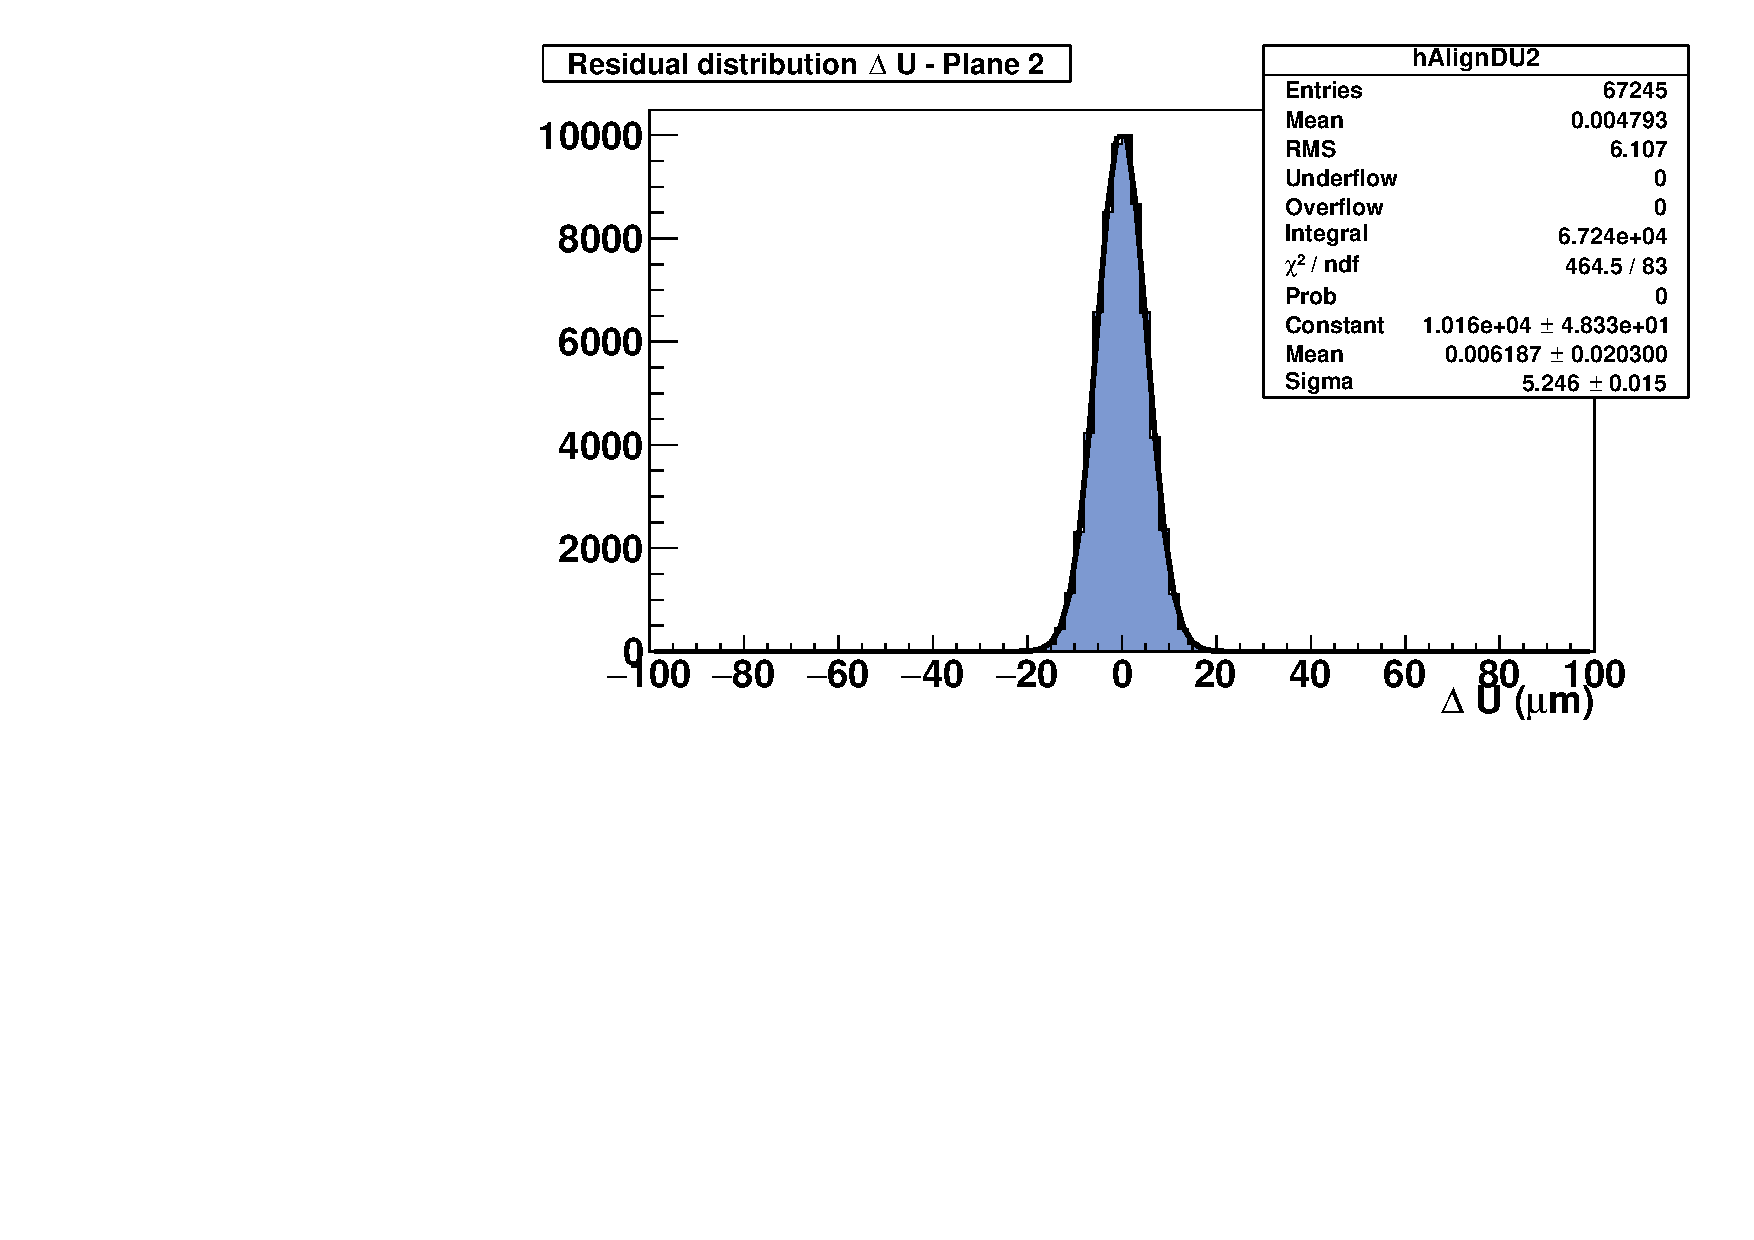
\includegraphics[width = 1.2\textwidth]{Pictures/deformation/residualUPl2_226056.pdf}
          \caption{Along $u$ direction.}
          \label{fig:alignmentPlane2}
        \end{subfigure}
        \hfill
         %add desired spacing between images, e. g. ~, \quad, \qquad, \hfill etc. 
          %(or a blank line to force the subfigure onto a new line)
        \begin{subfigure}[t]{0.45\textwidth}
          \centering
          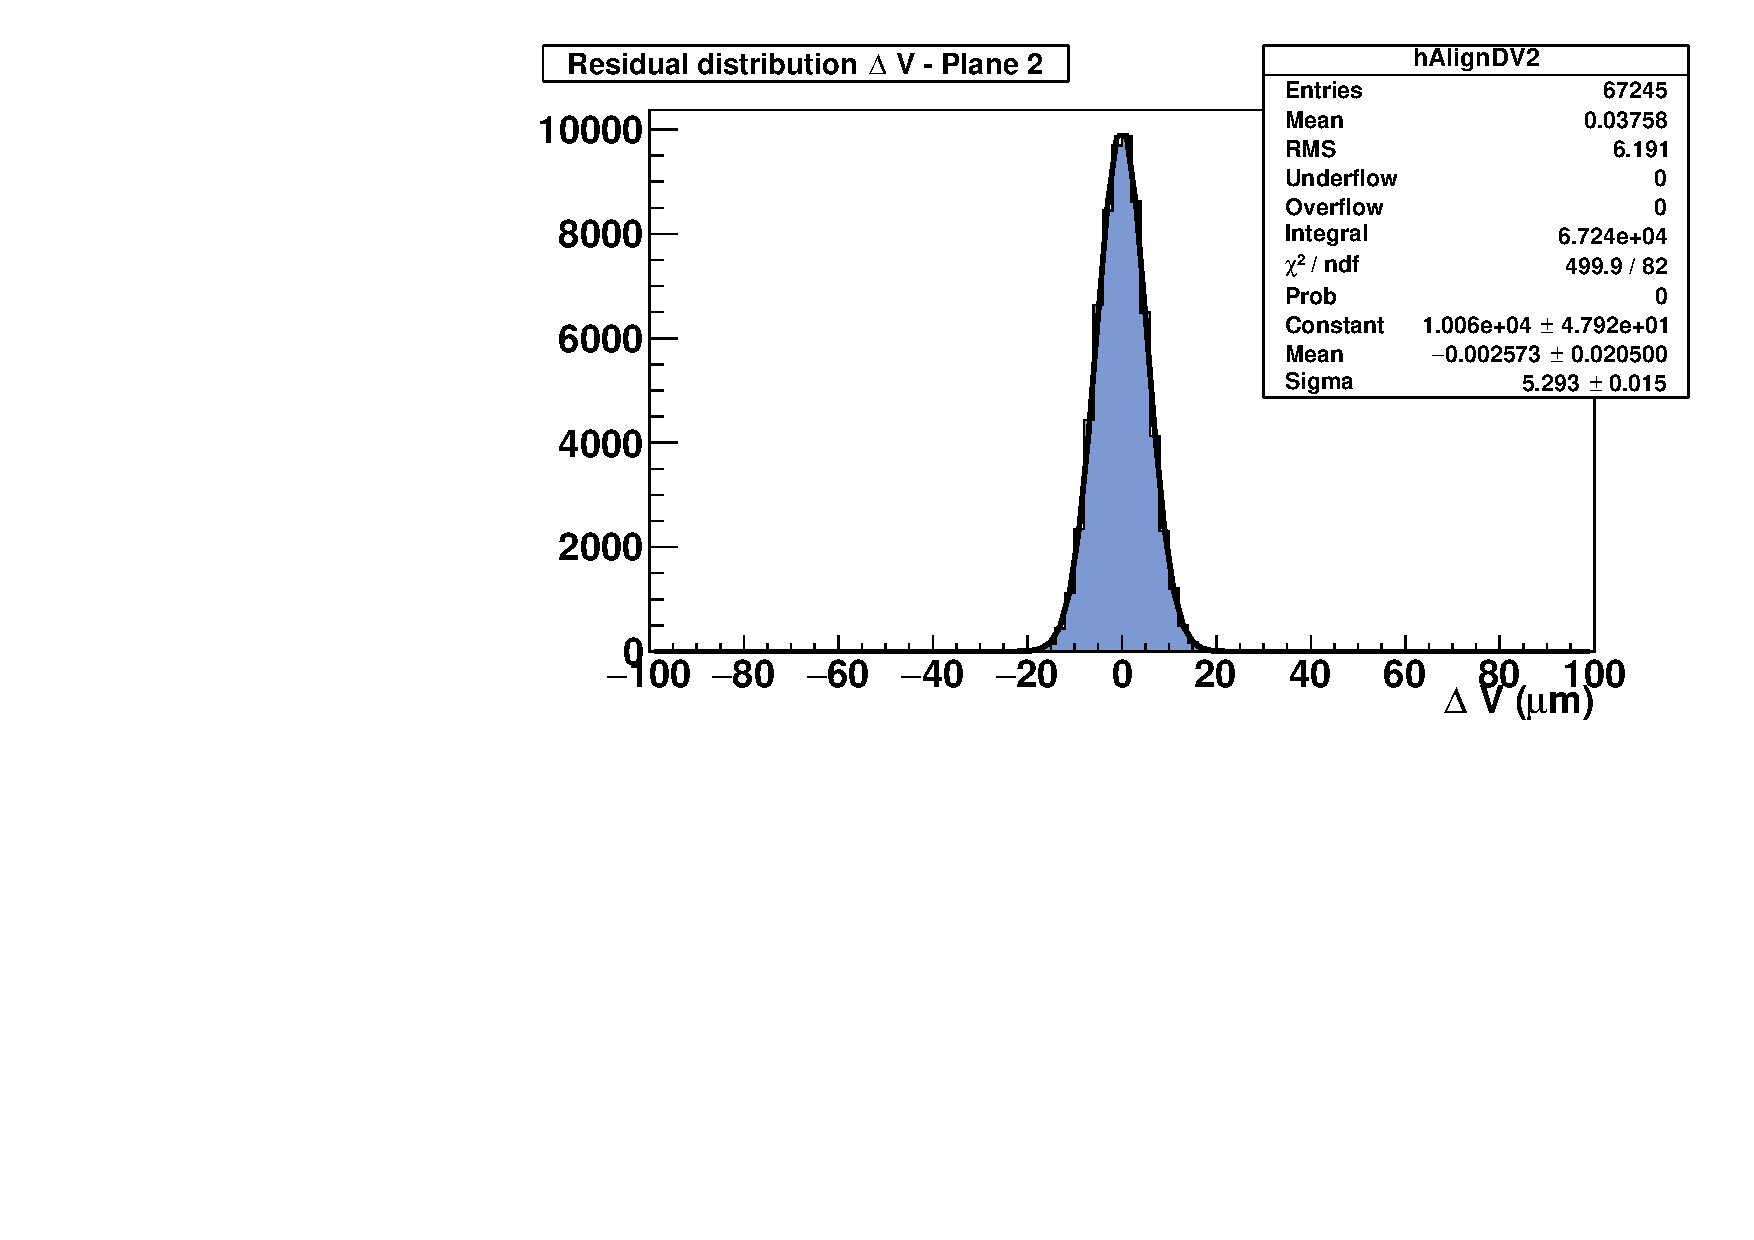
\includegraphics[width = 1.2\textwidth]{Pictures/deformation/residualVPl2_226056.pdf}
          \caption{Along $v$ direction.}
          \label{fig:alignmentPlane3}
        \end{subfigure}
        \caption{Residual distributions in the $u$ and $v$ directions for the middle telescope planes.}
        \label{fig:alignmentTelescope}
      \end{figure}

      As already explained, the alignment is an iterative procedure.
      At the beginning, a region of interest of $1000 \times 1000 \text{ }\mu\text{m}$ around the extrapolated is used to find a matching hit.
      Step by step, this region of interest is restricted to achieve a region of six times the pitch of the sensor.
      
      After aligning the telescope, a candidate track is dismissed if it is made of less than four hits or if the $\chi^2$ fit is greater than a fixed value determined by the user. 
      Two assumptions are used during the alignment. 
      The telescope planes are parallel each other.
      Thus the alignment consists of a translation along $x$ and $y$ and a rotation around the $z$-axis.
      As the test beam was performed without a magnetic field and pions of 120 GeV were used, the Coulomb multiple scattering is neglected.
      So, the tracks are perpendicular to the detectors and the alignment is not sensitive to the $z$ position.
      A precision of the millimeter level for the position does not have a huge impact on the alignment.

      \subsubsection{Alignment of the DUT}

      When the telescope alignment is done, the reference tracks reconstructed by the reference planes are used to align the \gls{DUT}.
      Its $z$ position is fixed, nonetheless, two degrees of freedom are added to the three degrees defined above: the rotations along the $x$ and $y$-axes.
      To assist the user in the alignment steps, several scatter plots are produced (see figure~\ref{fig:alignmentDUT}).
      For examples, figures~\ref{fig:alignUV} and~\ref{fig:alignVU} help to indicate a tilt in the $z$-direction, whereas figures~\ref{fig:alignUU} and~\ref{fig:alignVV} help to find shift and/or tilt in the respective $u$ and $v$-directions.
      Figures~\ref{fig:residualU} and~\ref{fig:residualV} show the residuals distribution in both direction for one sensor of the \gls{DUT}.
      The width of these distributions, called spatial residual $\sigma_{Res}$, is approximately 4.1 $\mu\text{m}$ and is a combination of the telescope resolution $\sigma_{tel}$, the multiple scattering $\sigma_{M.S}$ and the pointing resolution or spatial resolution of the sensor $\sigma_{DUT}$, as described in equation~\ref{eq:pointingResolution}.
      
      \begin{equation}
        \sigma_{Res}^2 = \sigma_{tel}^2 + \sigma_{DUT}^2 + \sigma_{M.S}^2
        \label{eq:pointingResolution}
      \end{equation}

      With 120 GeV pions, the effects of the Coulomb multiple scattering are neglected, thus the pointing resolution of the sensor is:

      \begin{equation}
        \sigma_{DUT} = \sqrt{\sigma_{Res}^2 - \sigma_{tel}^2}
      \end{equation}

      For the configuration of the telescope used, the spatial resolution of the whole system measured is $\sigma_{tel} \simeq 1.8 \text{ }\mu\text{m}$, thus the sensor studied here has a pointing resolution $\sigma_{DUT} \simeq 3.7 \text{ }\mu\text{m}$ for a threshold of 6 mV.
      This result is corroborating the pointing resolution of a single MIMOSA-26, as shown on figure~\ref{fig:mi26Perf} in chapter~\ref{chap:vxd}.

      \begin{figure}[H]
        \centering
        \begin{subfigure}[t]{0.45\textwidth}
          \centering
          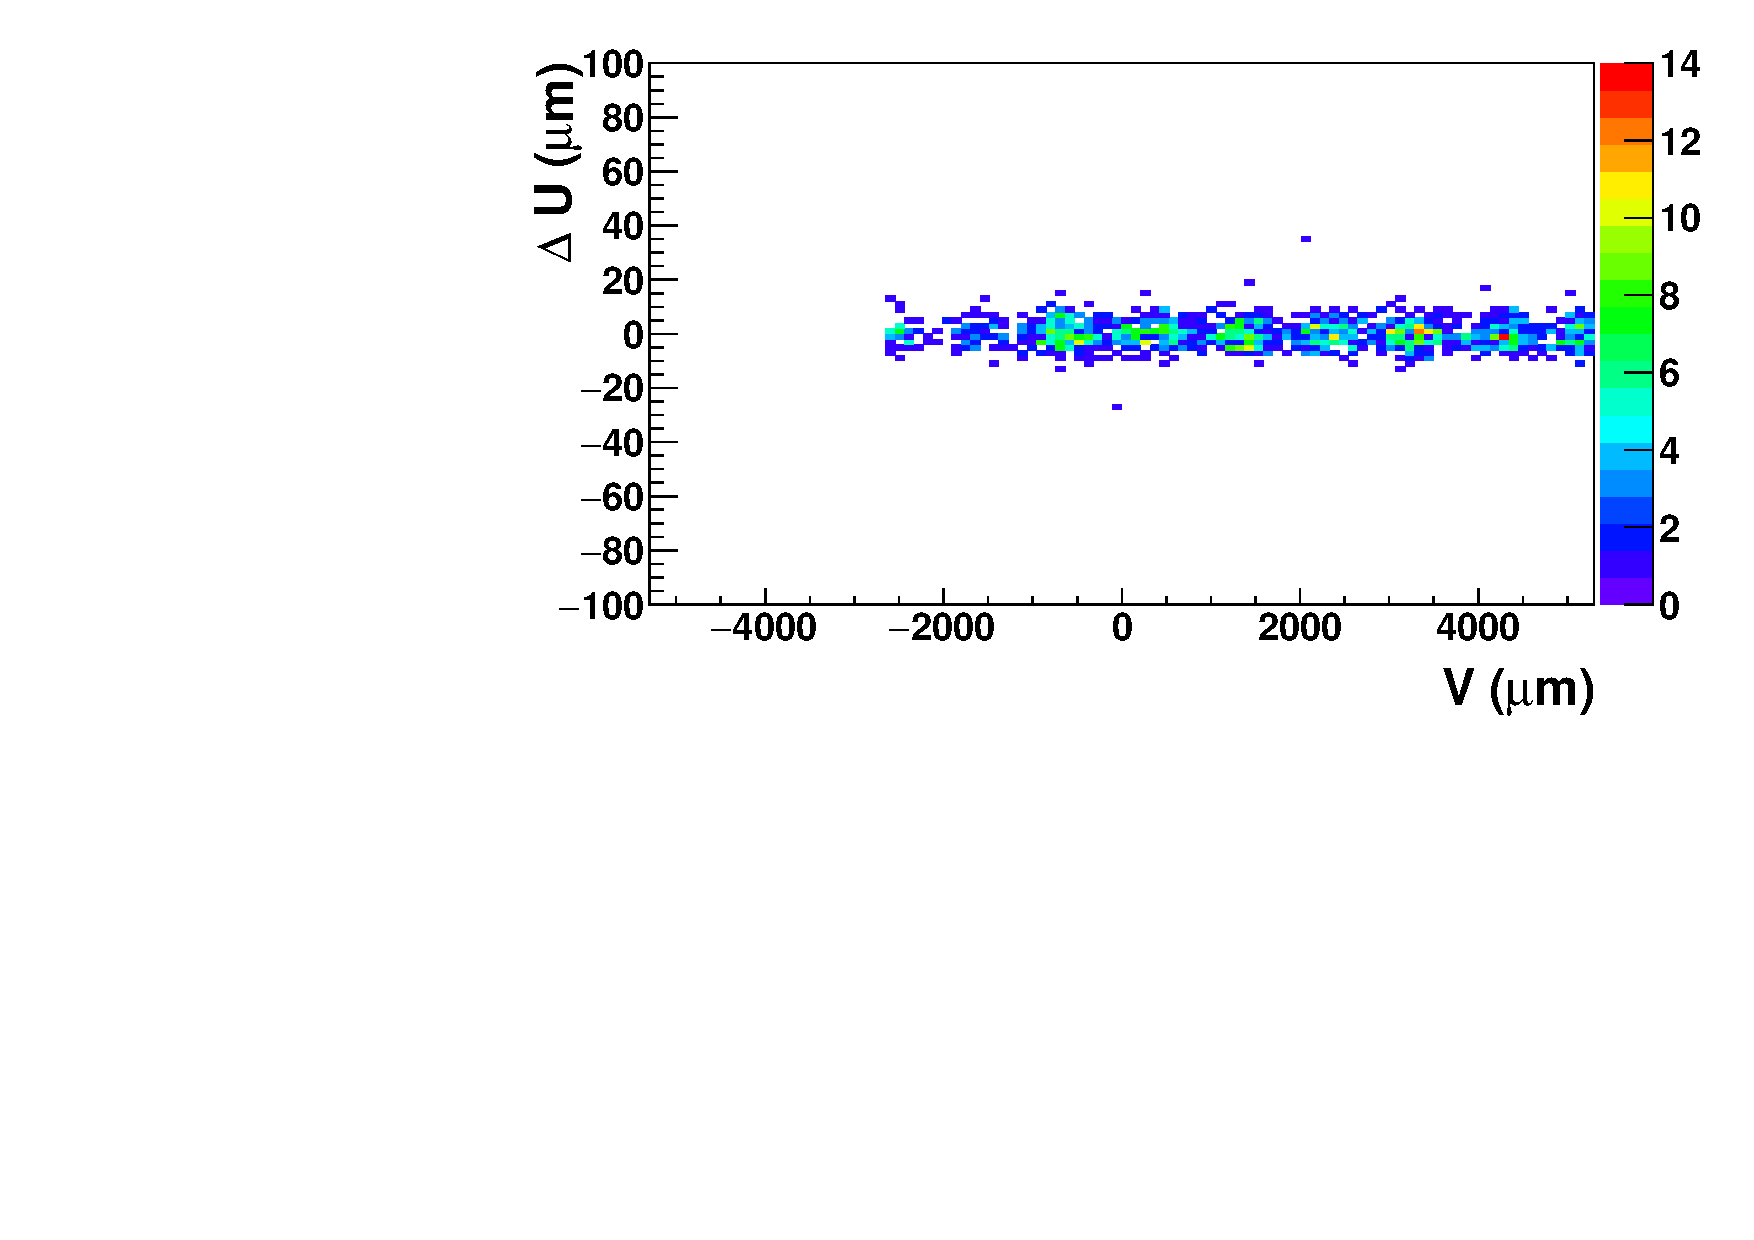
\includegraphics[width = 1.2\textwidth]{Pictures/deformation/deltaUV_6_normal_incidence.pdf}
          \caption{Along $u$ direction.}
          \label{fig:alignUV}
        \end{subfigure}
        \hfill
        \begin{subfigure}[t]{0.45\textwidth}
          \centering
          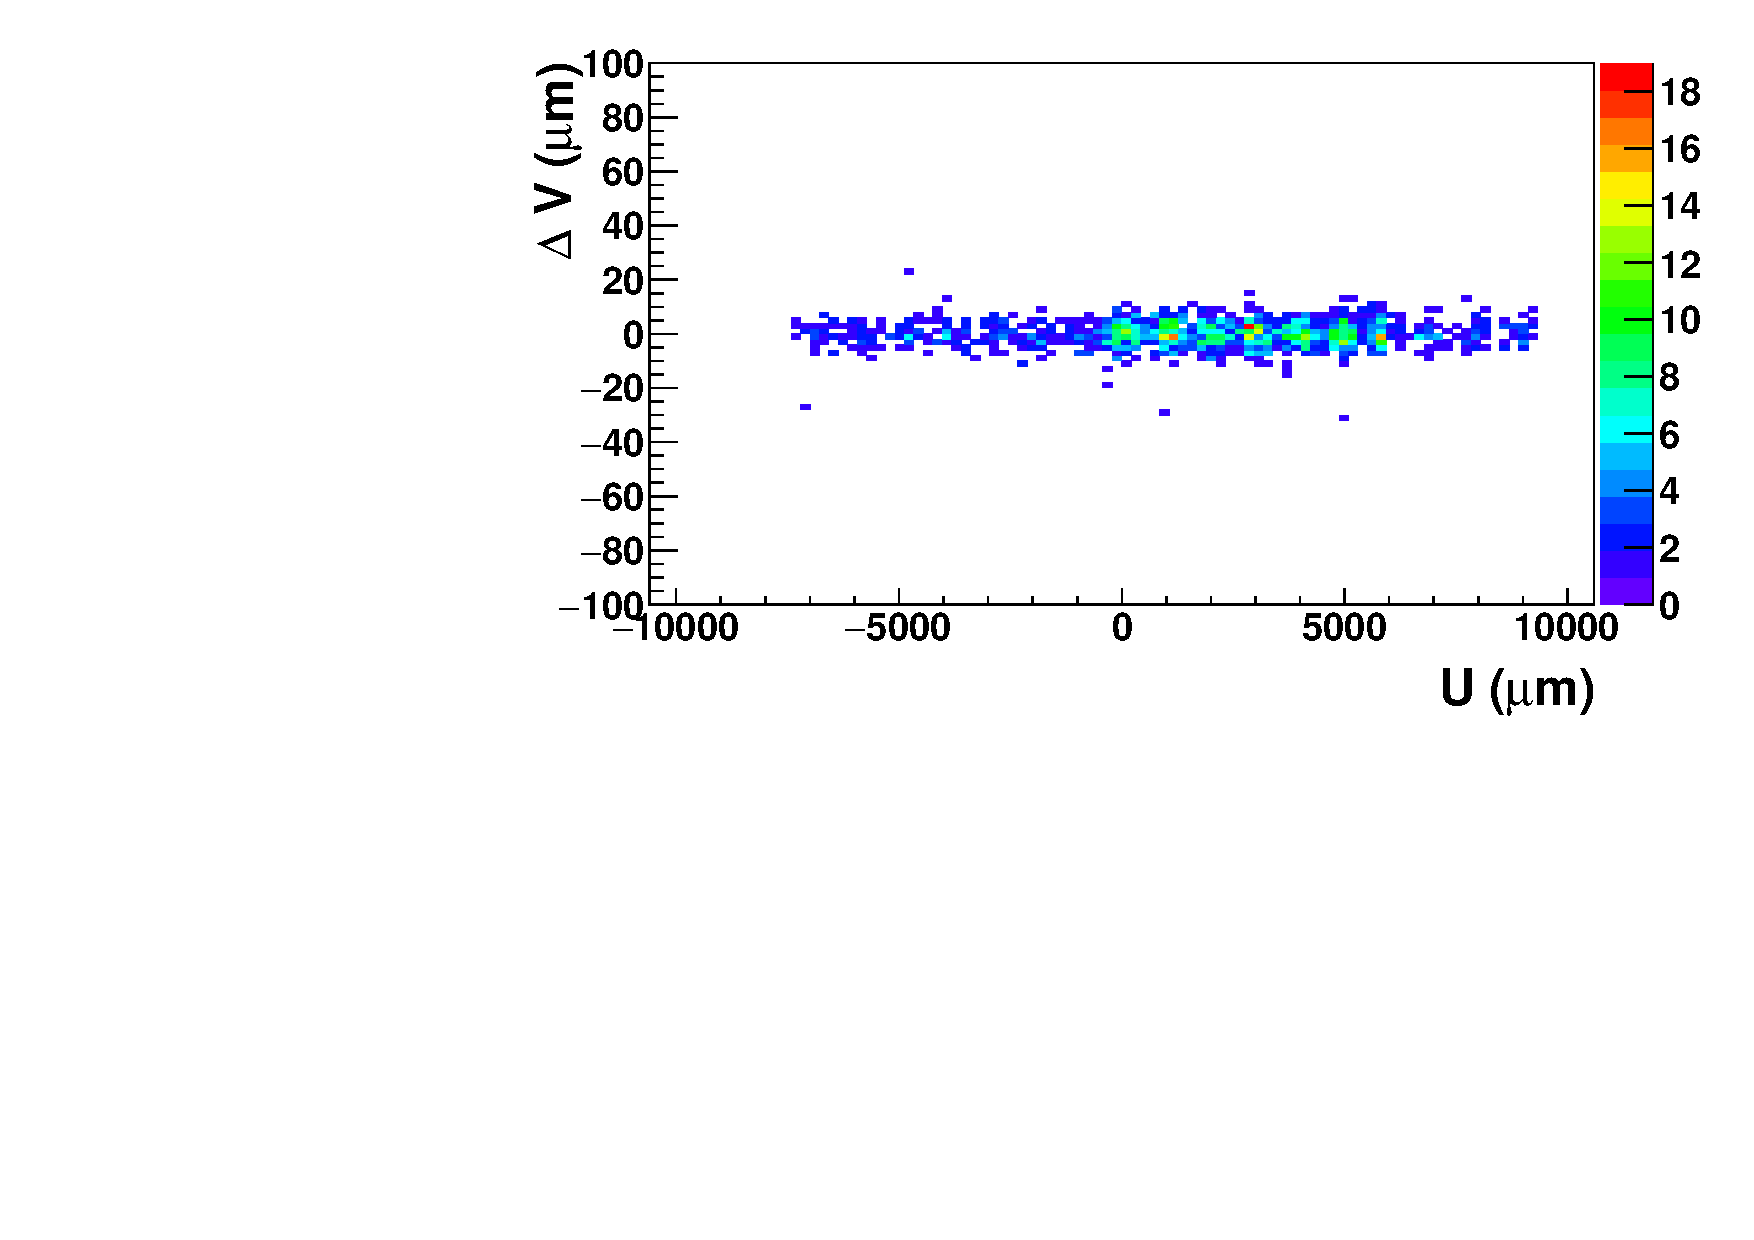
\includegraphics[width = 1.2\textwidth]{Pictures/deformation/deltaVU_6_normal_incidence.pdf}
          \caption{Along $v$ direction.}
          \label{fig:alignVU}
        \end{subfigure}
        
        \begin{subfigure}[t]{0.45\textwidth}
          \centering
          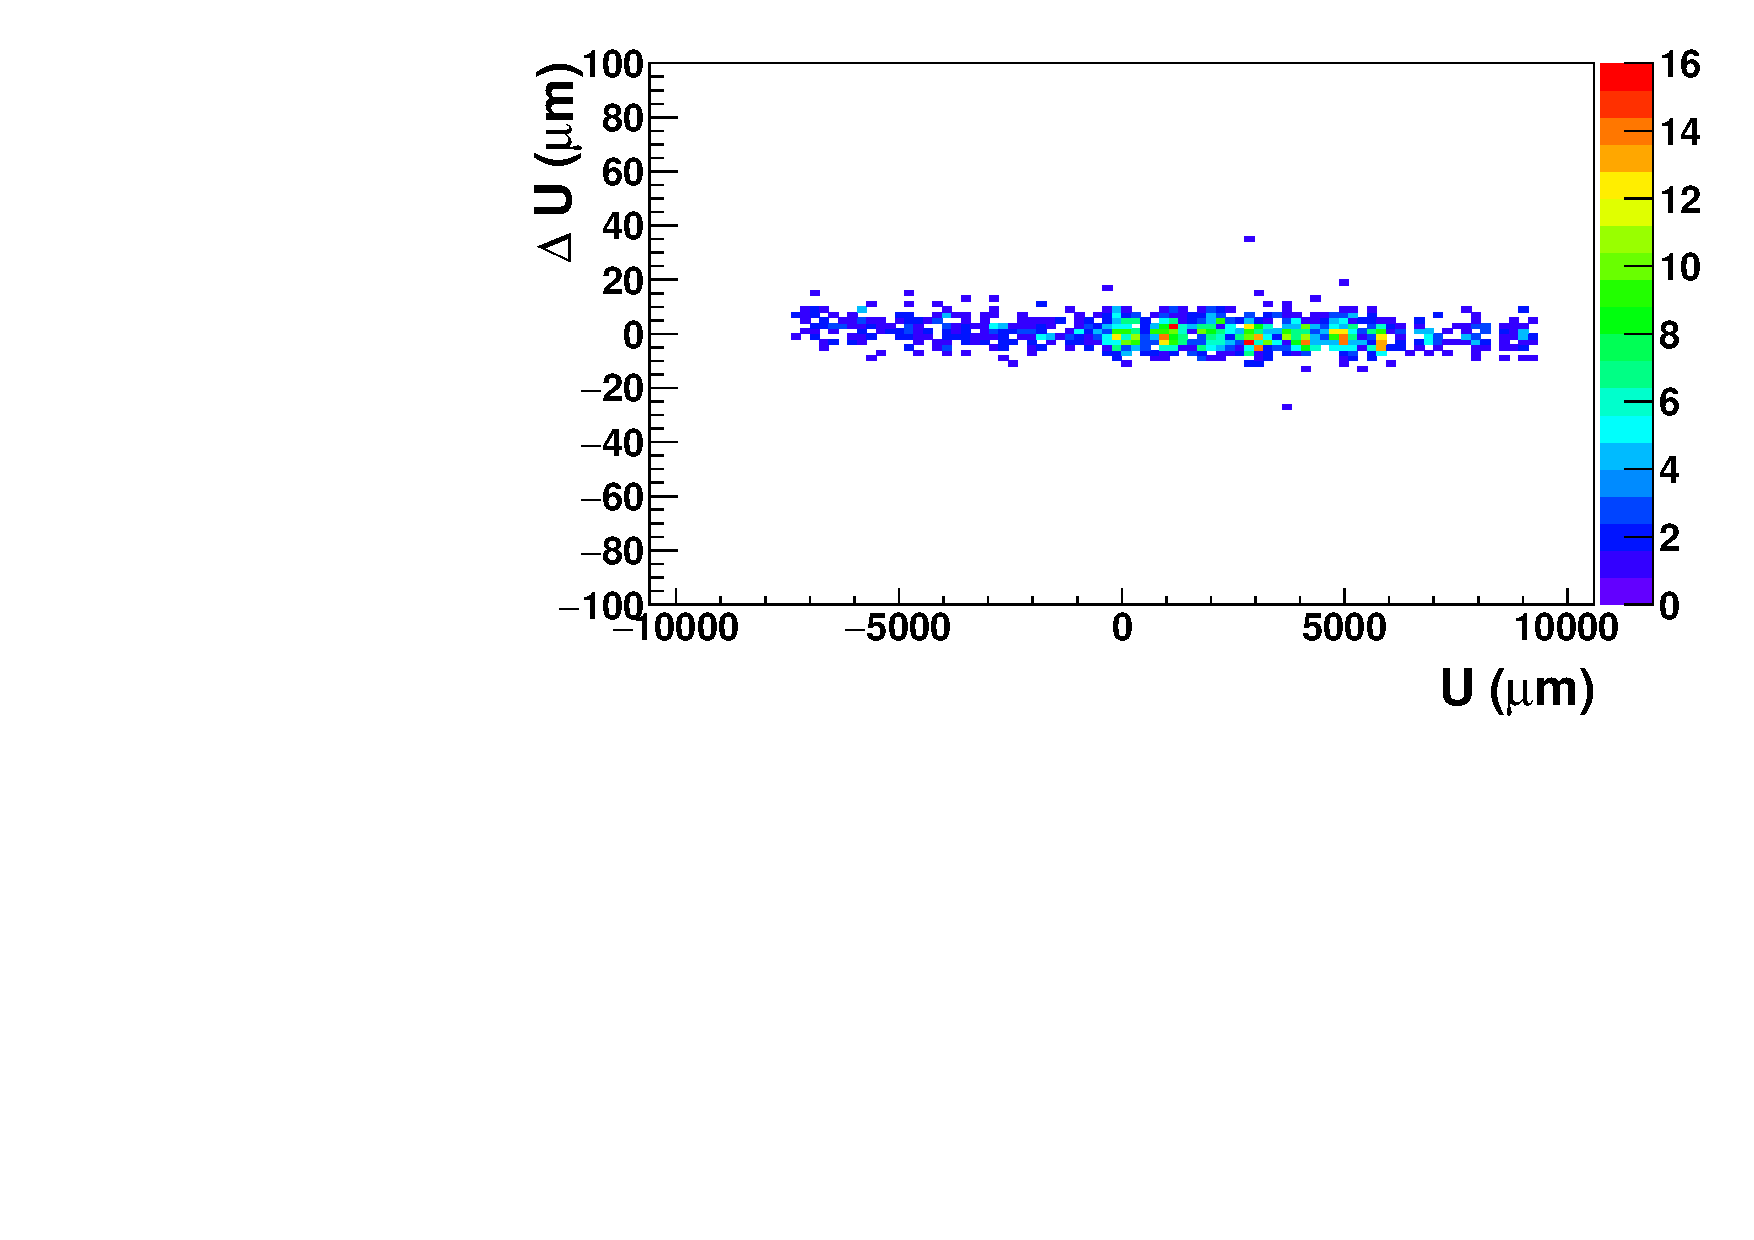
\includegraphics[width = 1.2\textwidth]{Pictures/deformation/deltaUU_6_normal_incidence.pdf}
          \caption{Along $u$ direction.}
          \label{fig:alignUU}
        \end{subfigure}
        \hfill
        \begin{subfigure}[t]{0.45\textwidth}
          \centering
          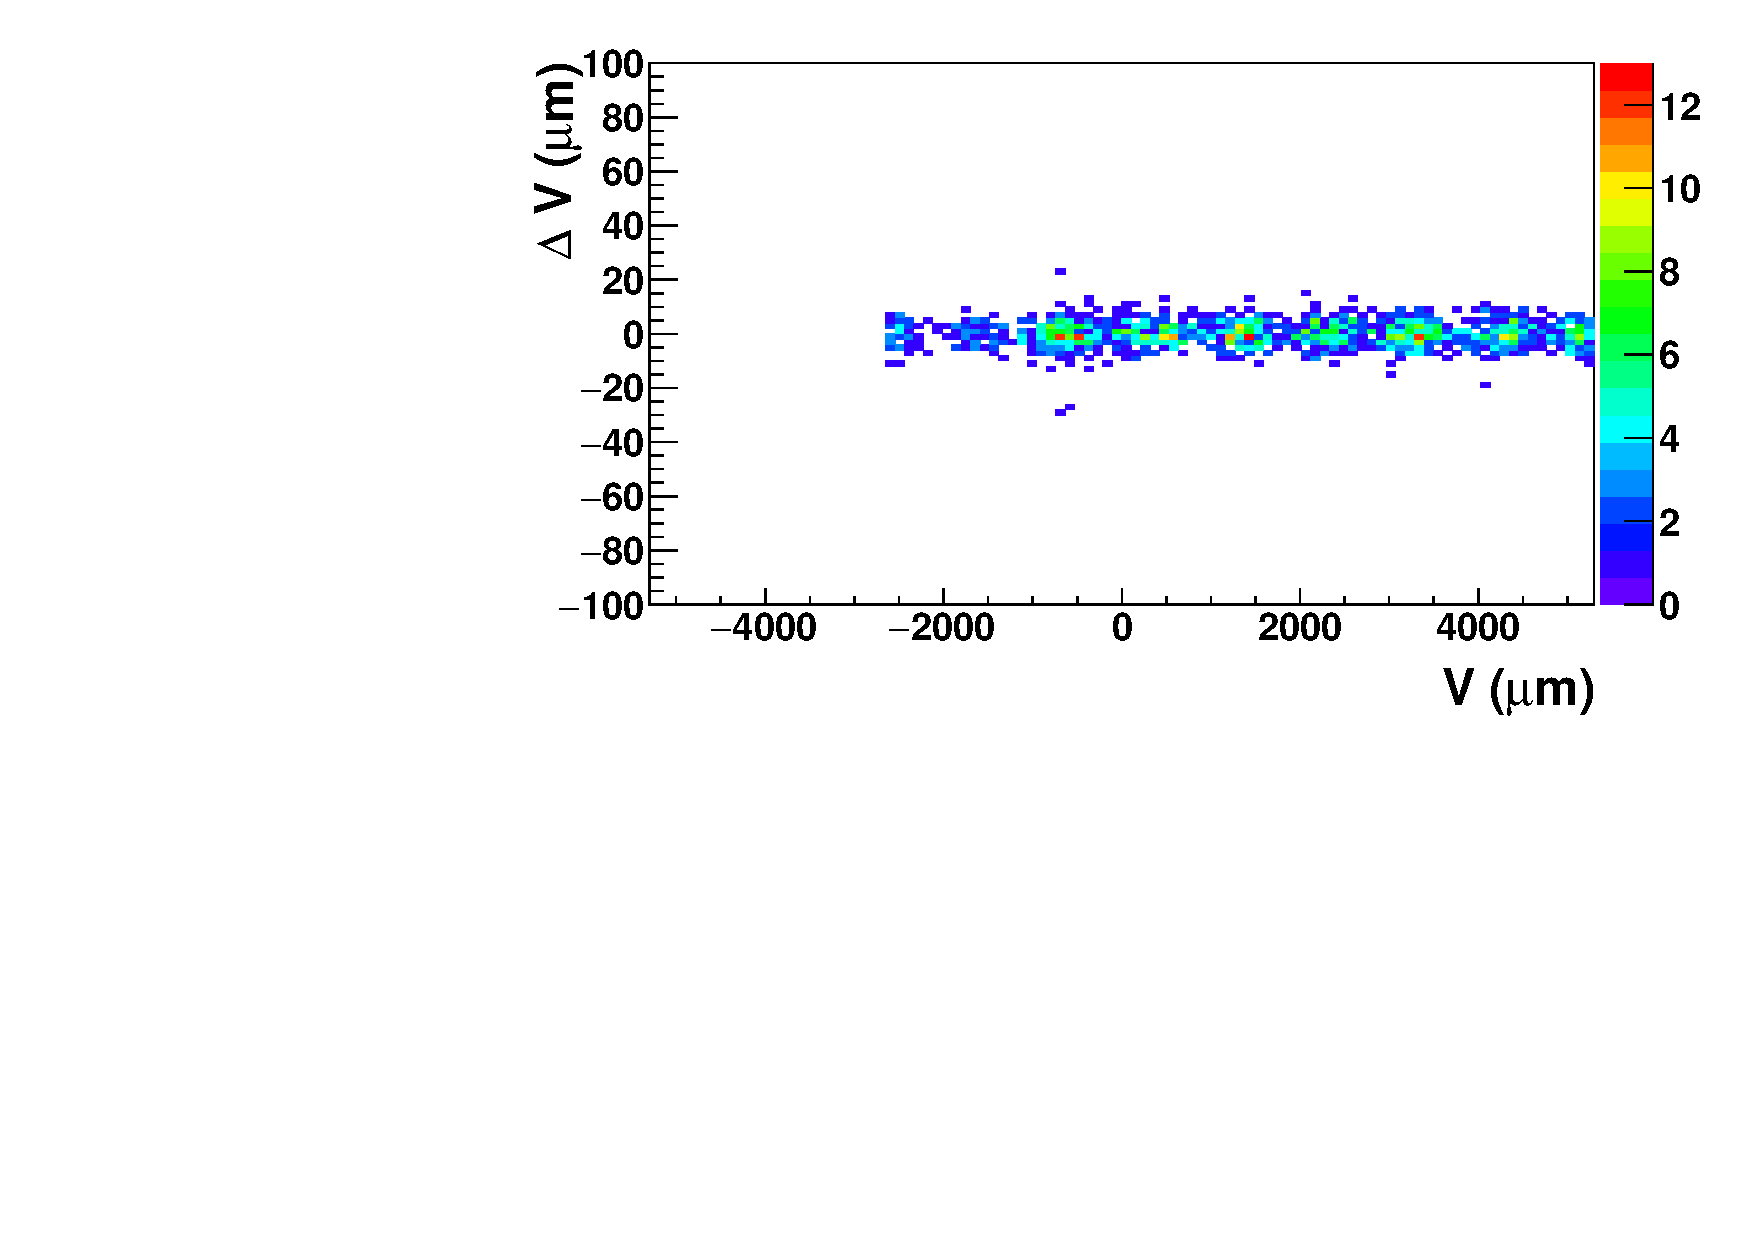
\includegraphics[width = 1.2\textwidth]{Pictures/deformation/deltaVV_6_normal_incidence.pdf}
          \caption{Along $v$ direction.}
          \label{fig:alignVV}
        \end{subfigure}

       \begin{subfigure}[t]{0.45\textwidth}
          \centering
          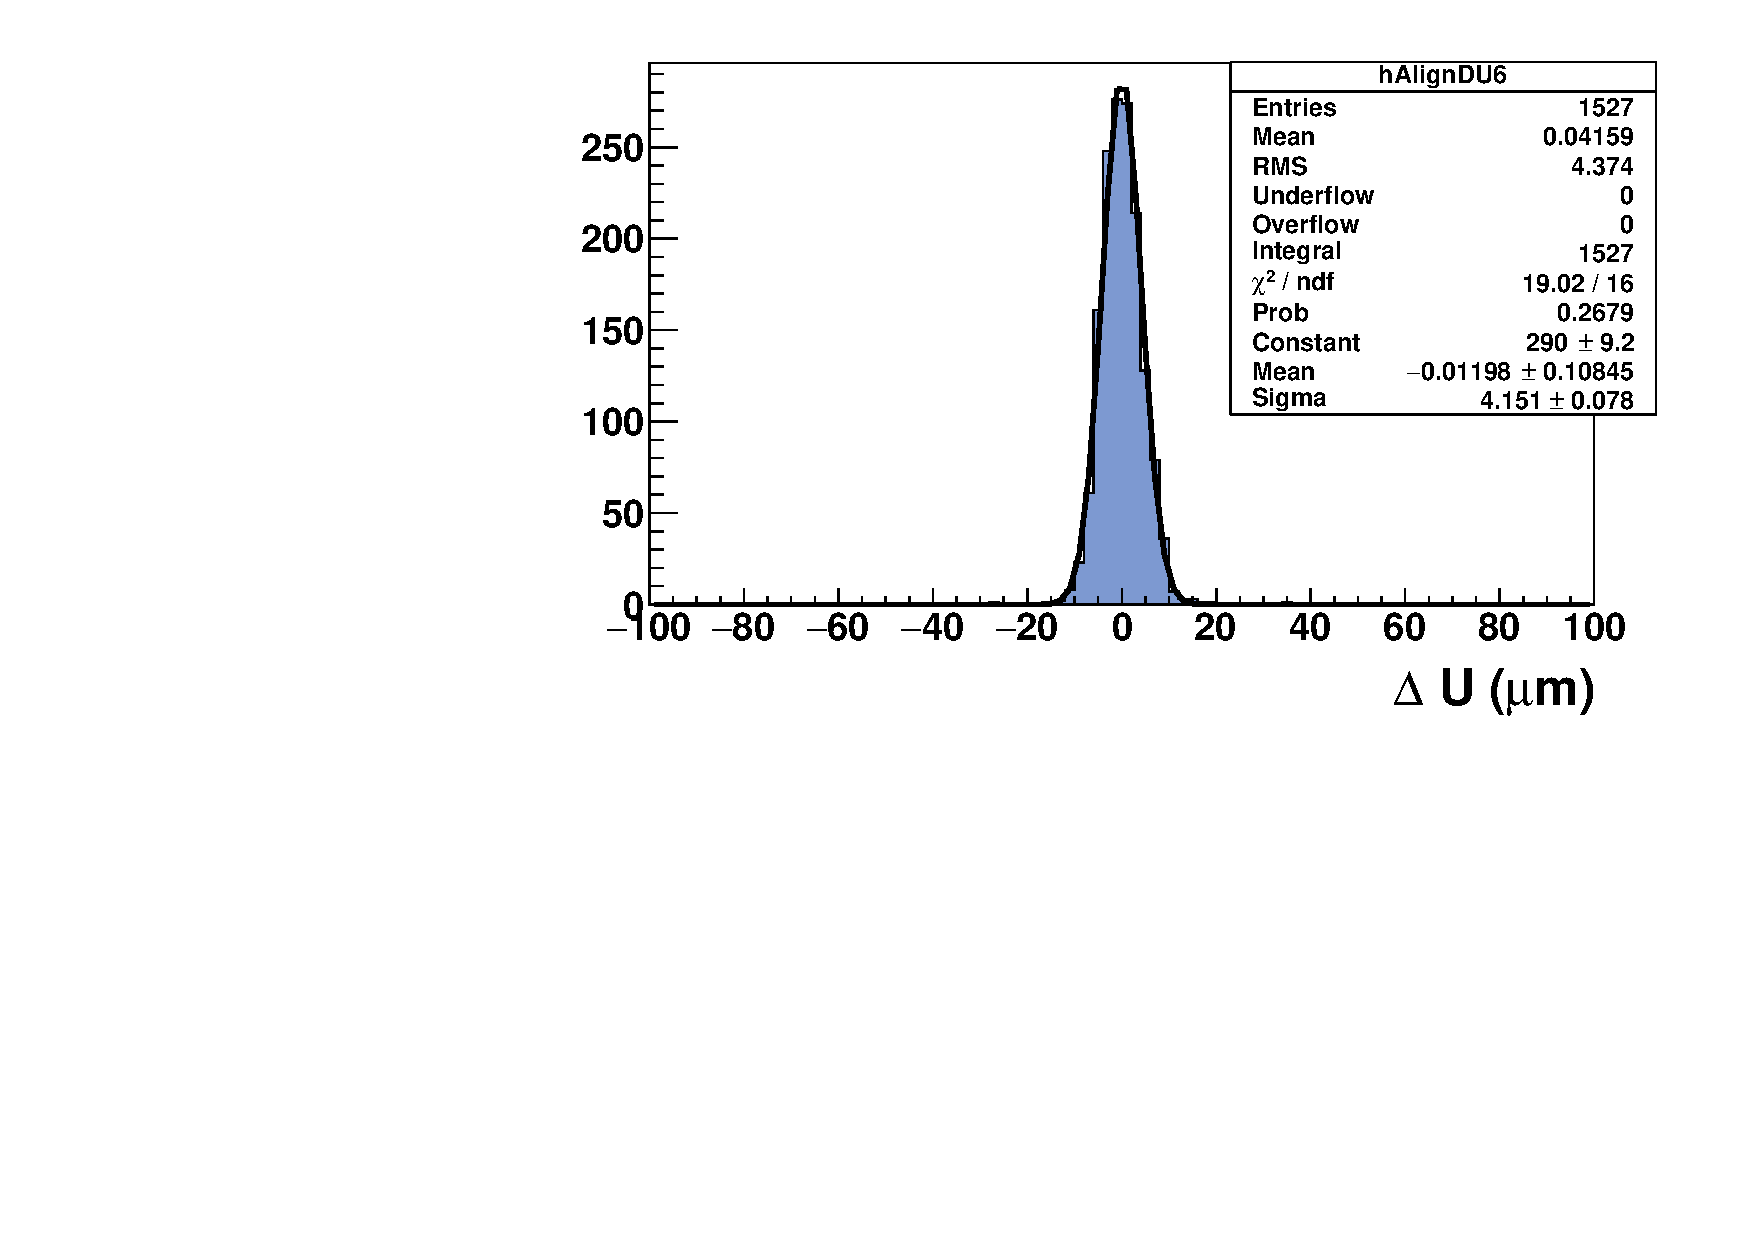
\includegraphics[width = 1.2\textwidth]{Pictures/deformation/deltaU_6_normal_incidence.pdf}
          \caption{Along $u$ direction.}
          \label{fig:residualU}
        \end{subfigure}
        \hfill
        \begin{subfigure}[t]{0.45\textwidth}
          \centering
          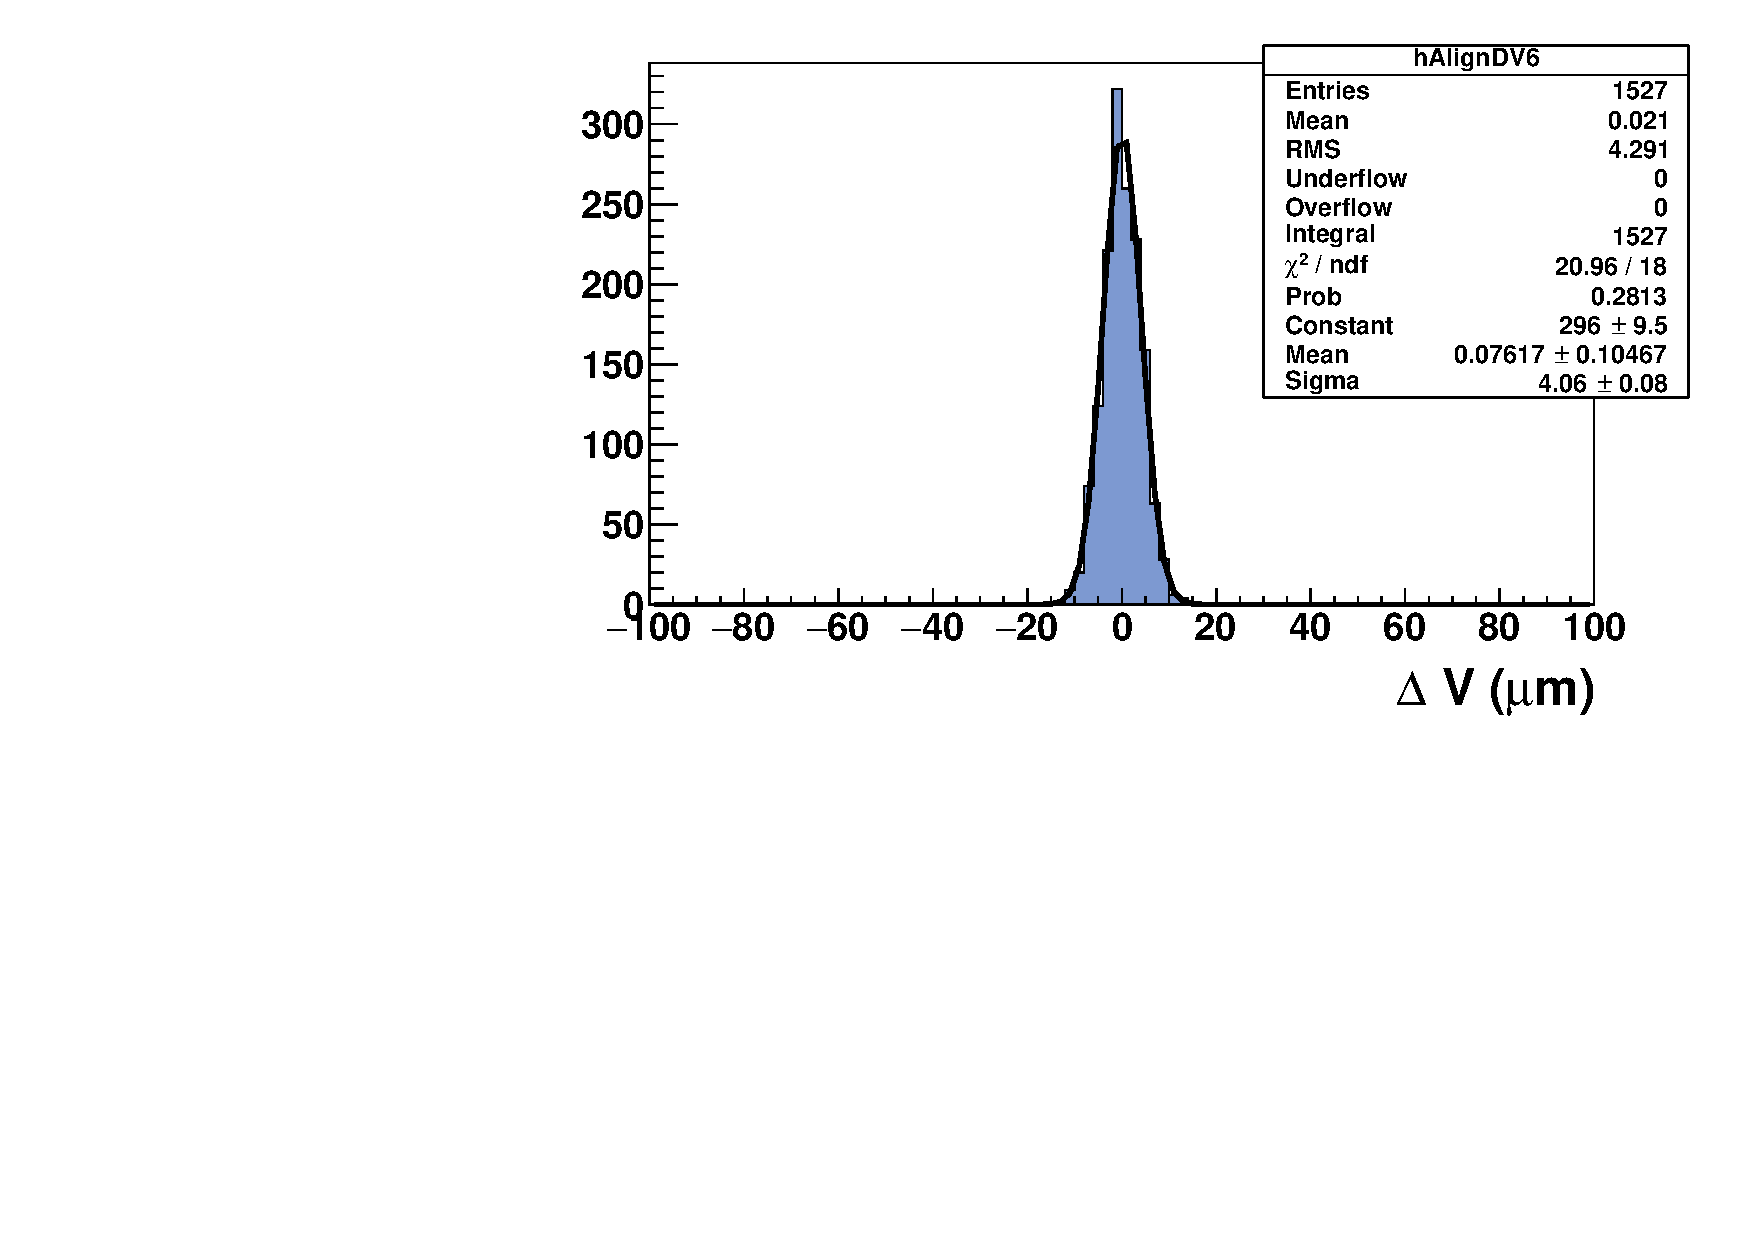
\includegraphics[width = 1.2\textwidth]{Pictures/deformation/deltaV_6_normal_incidence.pdf}
          \caption{Along $v$ direction.}
          \label{fig:residualV}
        \end{subfigure}
        \caption{Results of the DUT alignment: ~\ref{fig:alignUV} is the residual $\Delta U$ as a function of the hit position on the $v$-direction, ~\ref{fig:alignVU} is the residual $\Delta V$ as a function of the hit position on the $u$-direction, ~\ref{fig:alignUU} is the residual $\Delta U$ as a function of the hit position on the same direction, ~\ref{fig:alignVV} is the same plot for the other direction,~\ref{fig:residualU} and~\ref{fig:residualV} are the residuals distributions in the two directions.}
        \label{fig:alignmentDUT}
      \end{figure}

    \subsection{Ladder tilted in one direction}
    \label{subsec:deformation}

      The performances of the \gls{DUT} are also studied for tilted tracks by rotating the ladder with respect to the beam axis along the $v$-direction.
      Three different angles were tested ($28^{\degree}$, $36^{\degree}$ and $60^{\degree}$), as well as different threshold cuts and air flow speed. 
      The results presented below are for a run with a $36^{\degree}$ tilt, a threshold sets to 5 mV and an air flow speed of 3 $\text{m.s}^{-1}$.
      The same alignment procedure as presented in the subsection above is used, nevertheless, the alignment of the plane along the $u$-direction is more complicated than the other direction.
      The scatter plot in the $v$-direction for the front plane which is shown on figure~\ref{fig:scatterDVV_deformed} represents a good alignment and the spatial residual (see figure~\ref{fig:residualVDef}) is comparable to the one find for normal incidence tracks.
      But, the scatter plot $\Delta u=f(u_{hit})$ as presented on figure~\ref{fig:scatterDUU_deformed} shows a banana shape that can not be flatten with a traditional alignment procedure.
      Moreover, the spatial residual measured on figure~\ref{fig:residualUDef} is larger (6.8 $\mu\text{m}$ instead of $\sim 4 \text{ }\mu\text{m}$ in the $v$-direction) and the distribution has a large tail on the positive values.
      Concerning the back plane, the deformation is also visible on figure~\ref{fig:scatterDUU_deformed_back} but have a different form.
      The spatial residual measured for this plane is more than two times larger than the other side (14.1 $\mu\text{m}$) as it is depicted on figure~\ref{fig:residualUDef_back}.

      \begin{figure}[!h]
        \centering
        \begin{subfigure}[t]{0.45\textwidth}
          \centering
          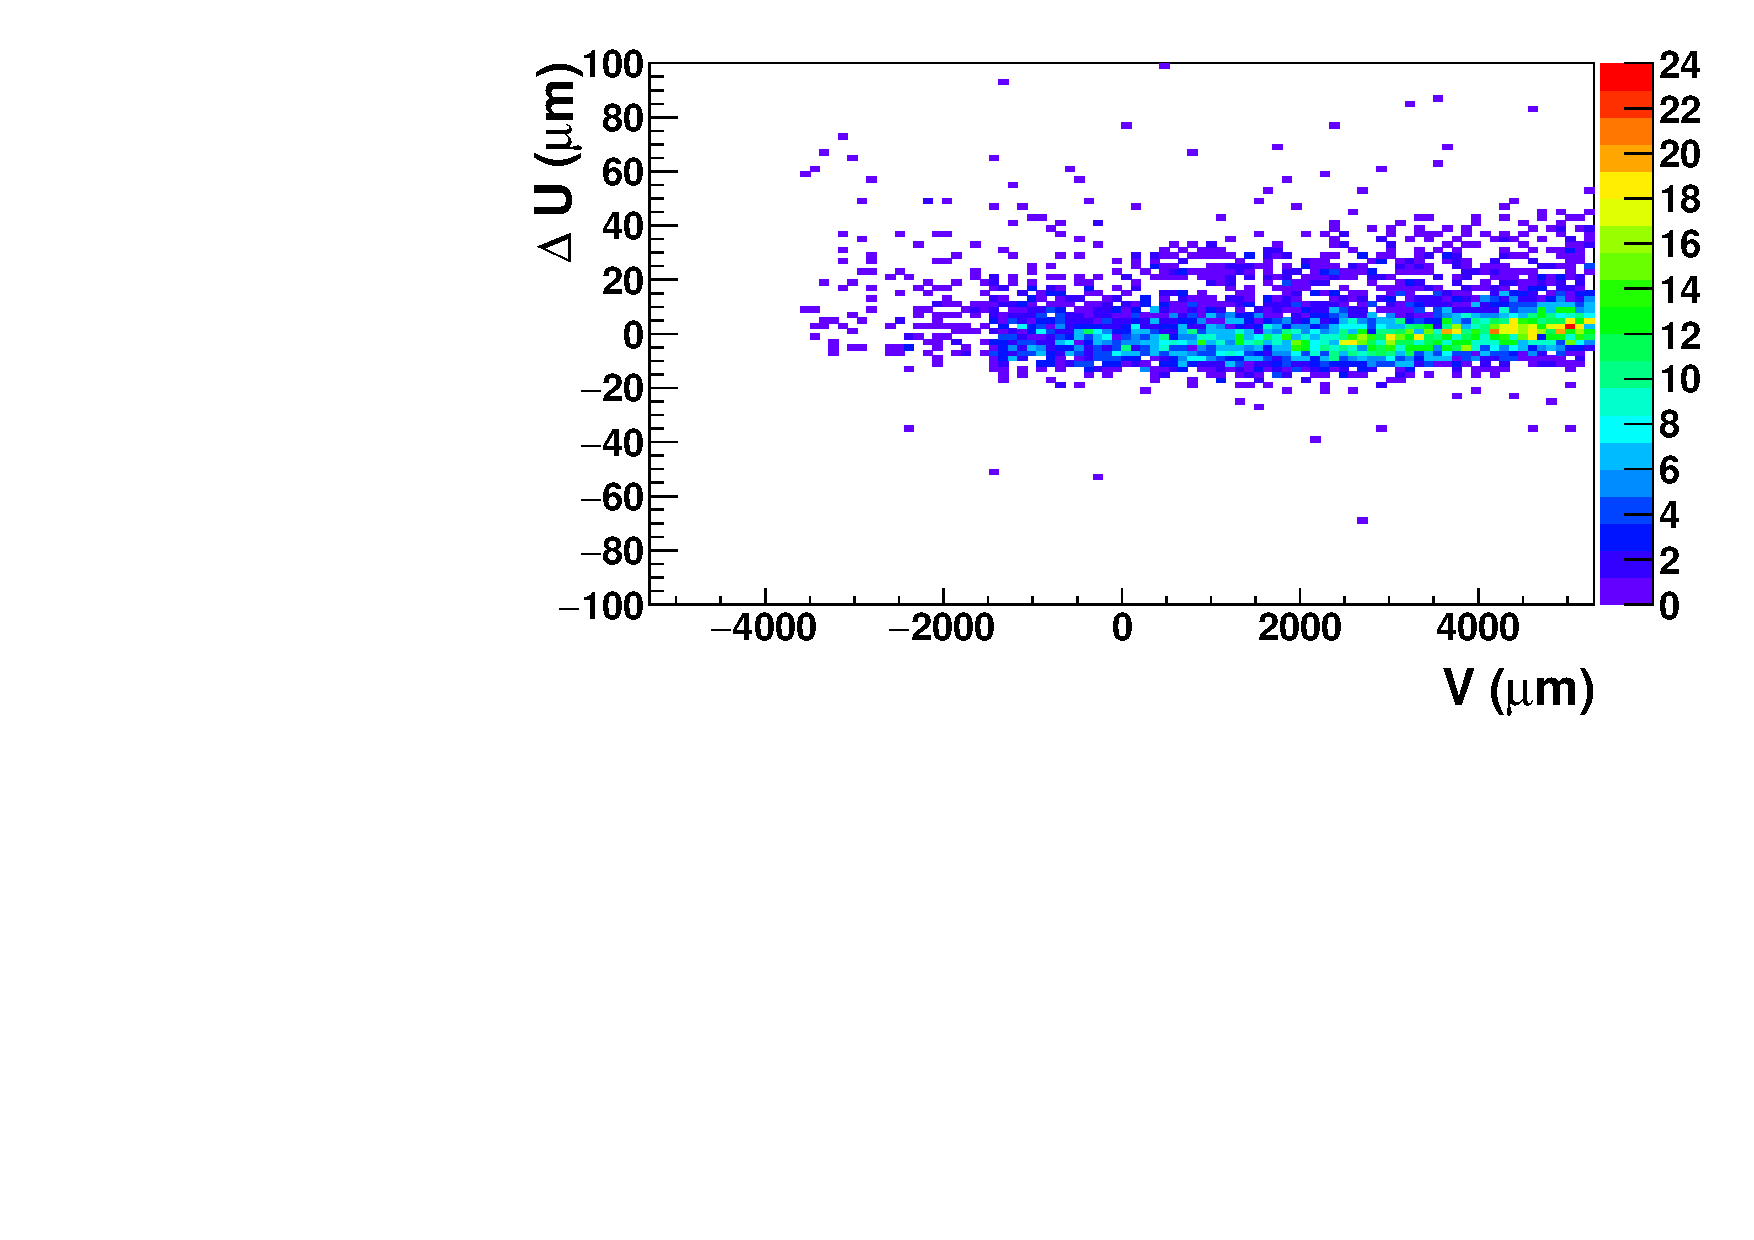
\includegraphics[width = 1.2\textwidth]{Pictures/deformation/deltaUV_8_deformed.pdf}
          \caption{}
          \label{fig:scatterDUV_deformed}
        \end{subfigure}
        \hfill
        \begin{subfigure}[t]{0.45\textwidth}
          \centering
          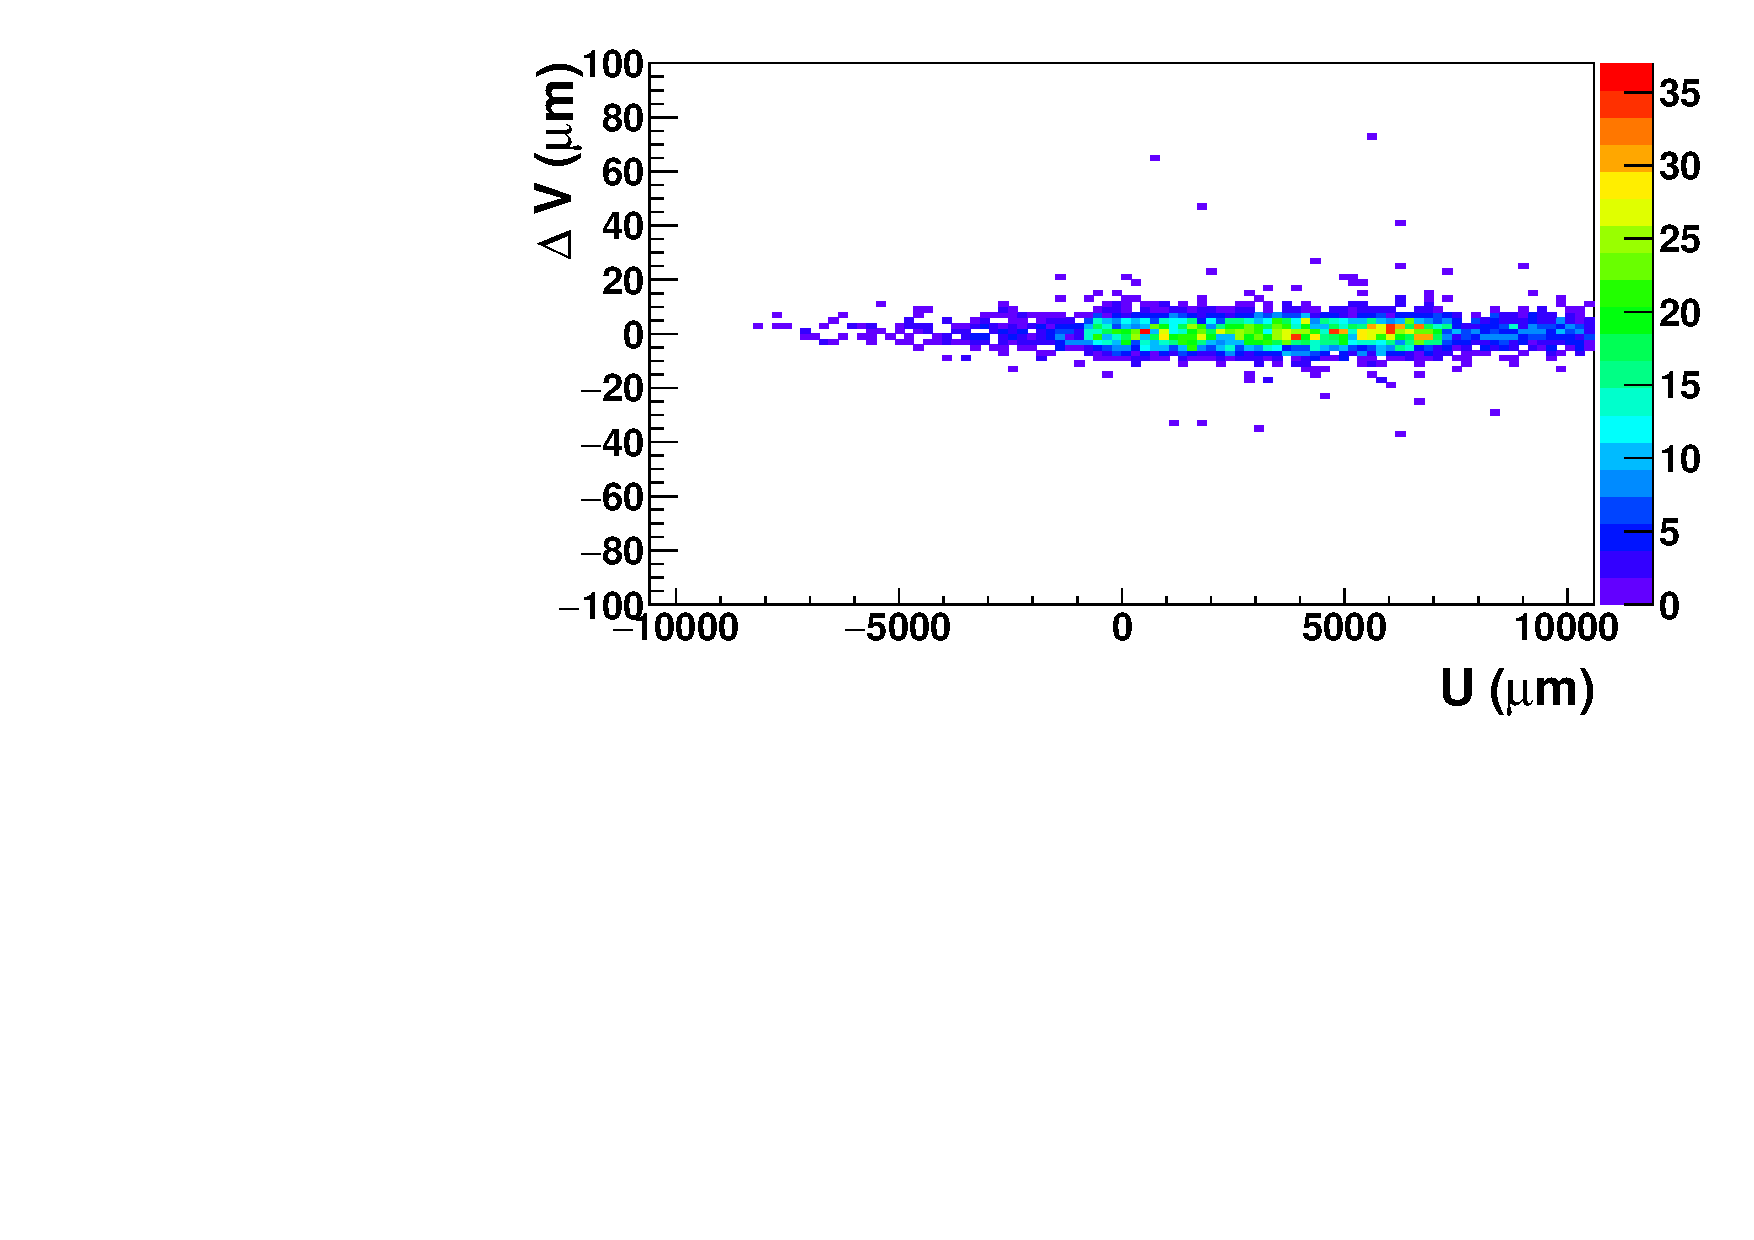
\includegraphics[width = 1.2\textwidth]{Pictures/deformation/deltaVU_8_deformed.pdf}
          \caption{}
          \label{fig:scatterDVU_deformed}
        \end{subfigure}

        \begin{subfigure}[t]{0.45\textwidth}
          \centering
          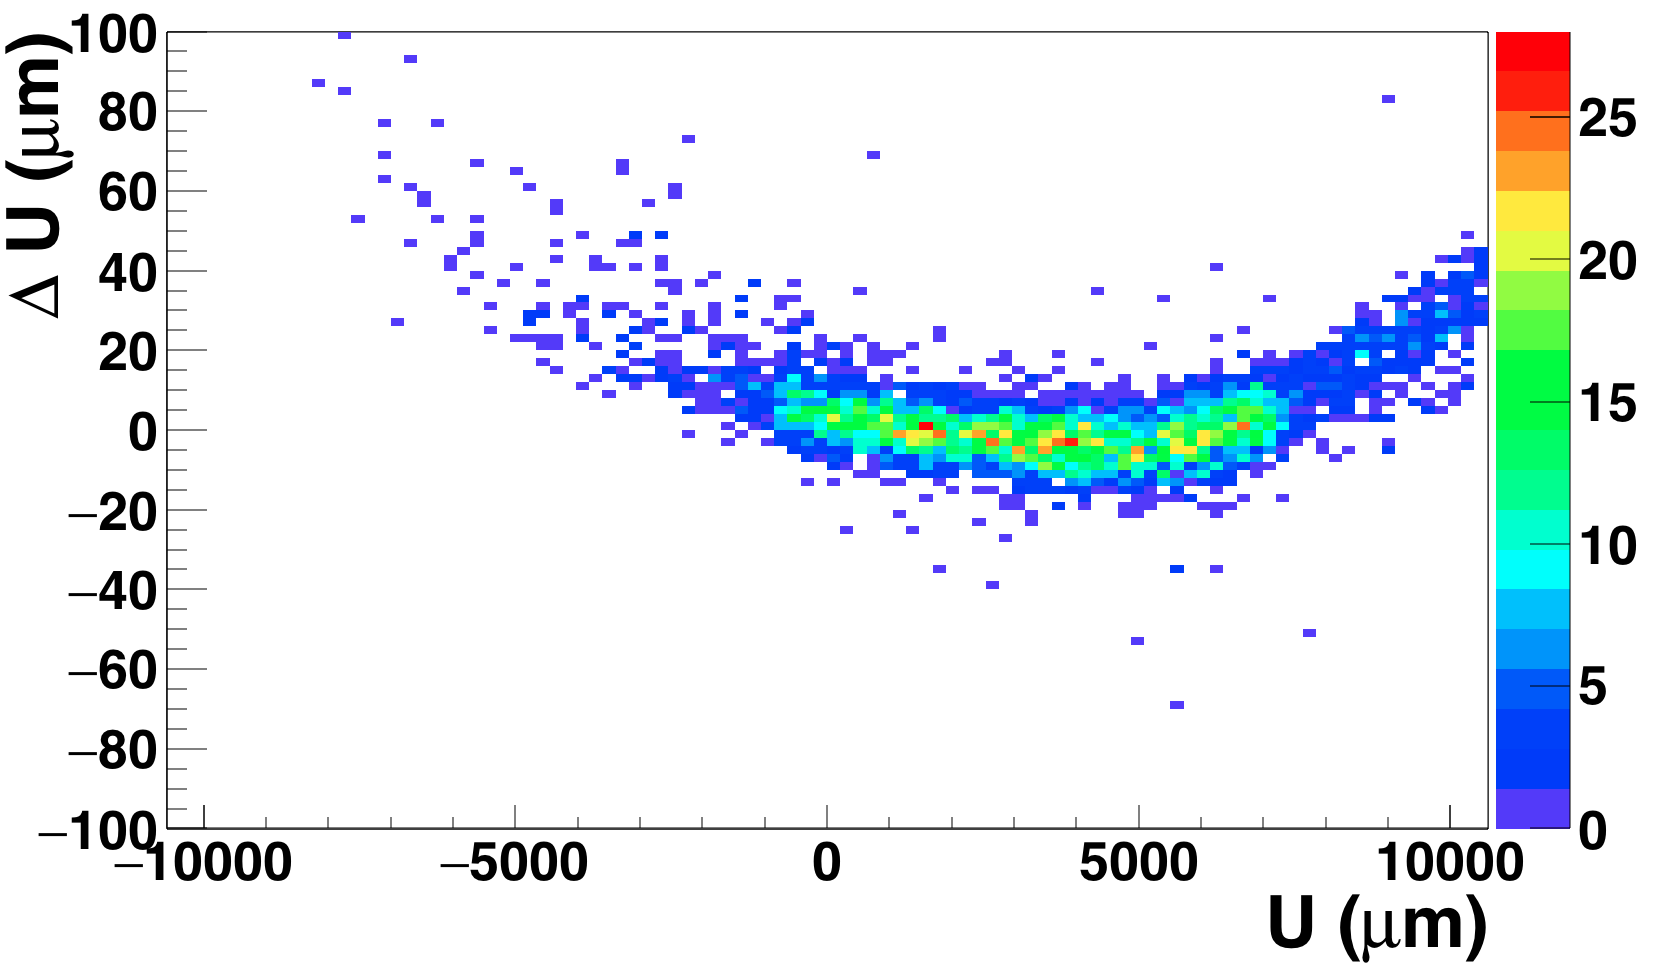
\includegraphics[width = 1.2\textwidth]{Pictures/deformation/deltaUU_8_deformed.png}
          \caption{}
          \label{fig:scatterDUU_deformed}
        \end{subfigure}
        \hfill
        \begin{subfigure}[t]{0.45\textwidth}
          \centering
          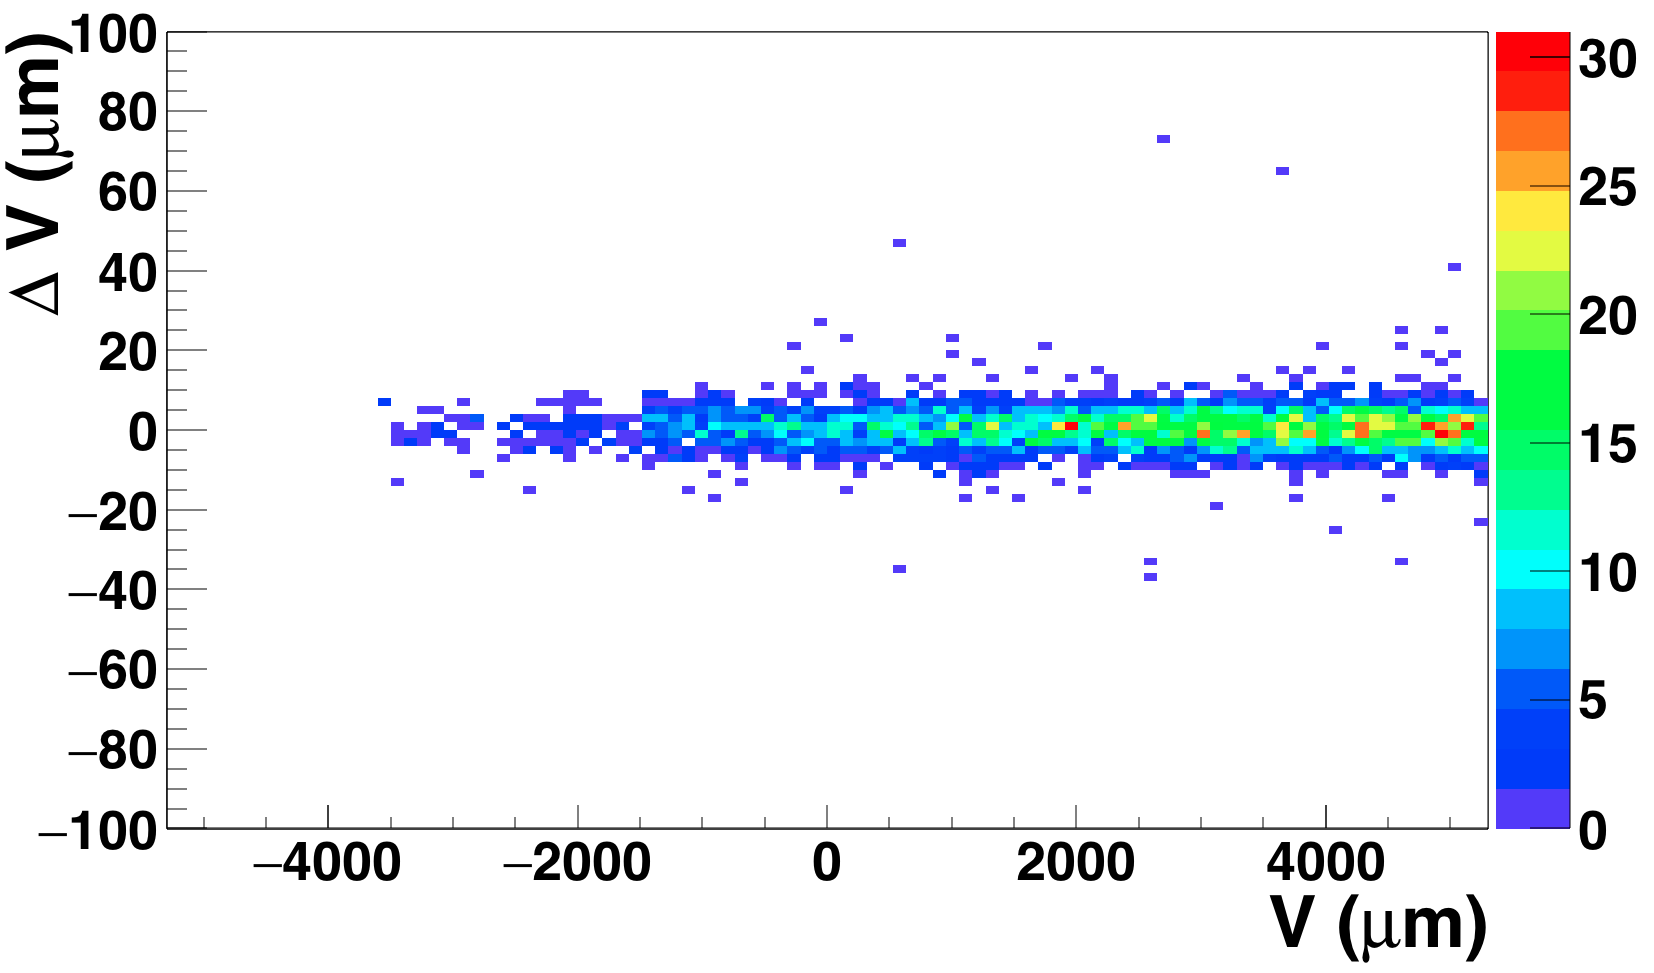
\includegraphics[width = 1.2\textwidth]{Pictures/deformation/deltaVV_8_deformed.png}
          \caption{}
          \label{fig:scatterDVV_deformed}
        \end{subfigure}

        \begin{subfigure}[t]{0.45\textwidth}
          \centering
          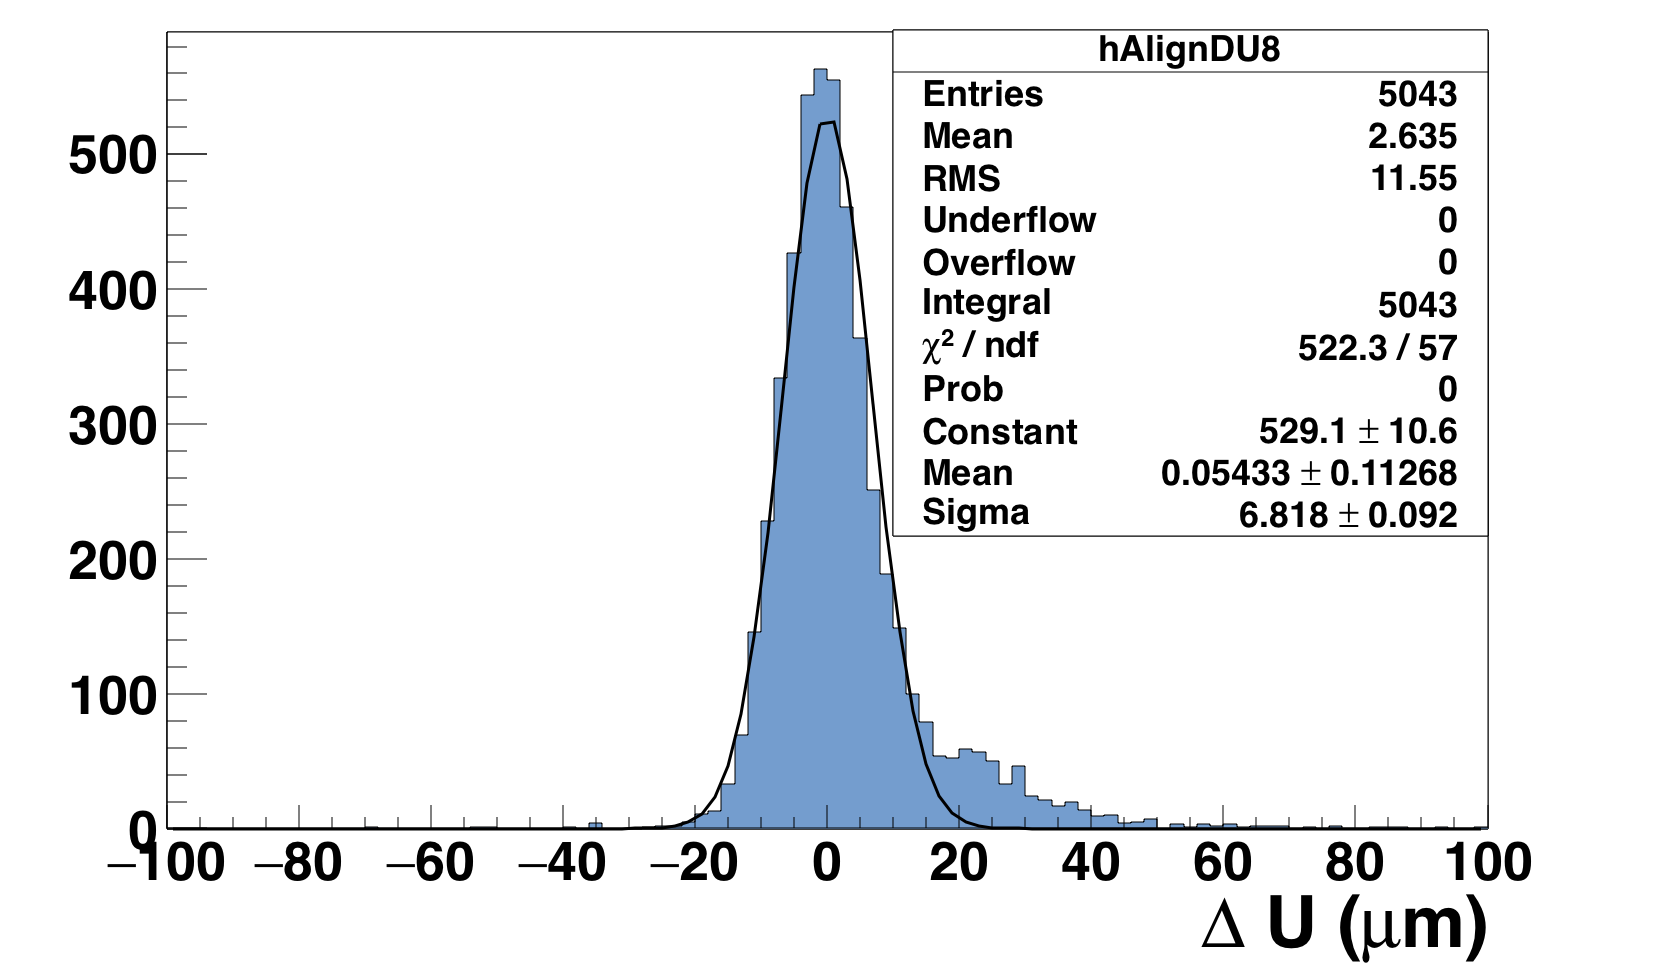
\includegraphics[width = 1.2\textwidth]{Pictures/deformation/deltaU_8_deformed.png}
          \caption{}
          \label{fig:residualUDef}
        \end{subfigure}
        \hfill
        \begin{subfigure}[t]{0.45\textwidth}
          \centering
          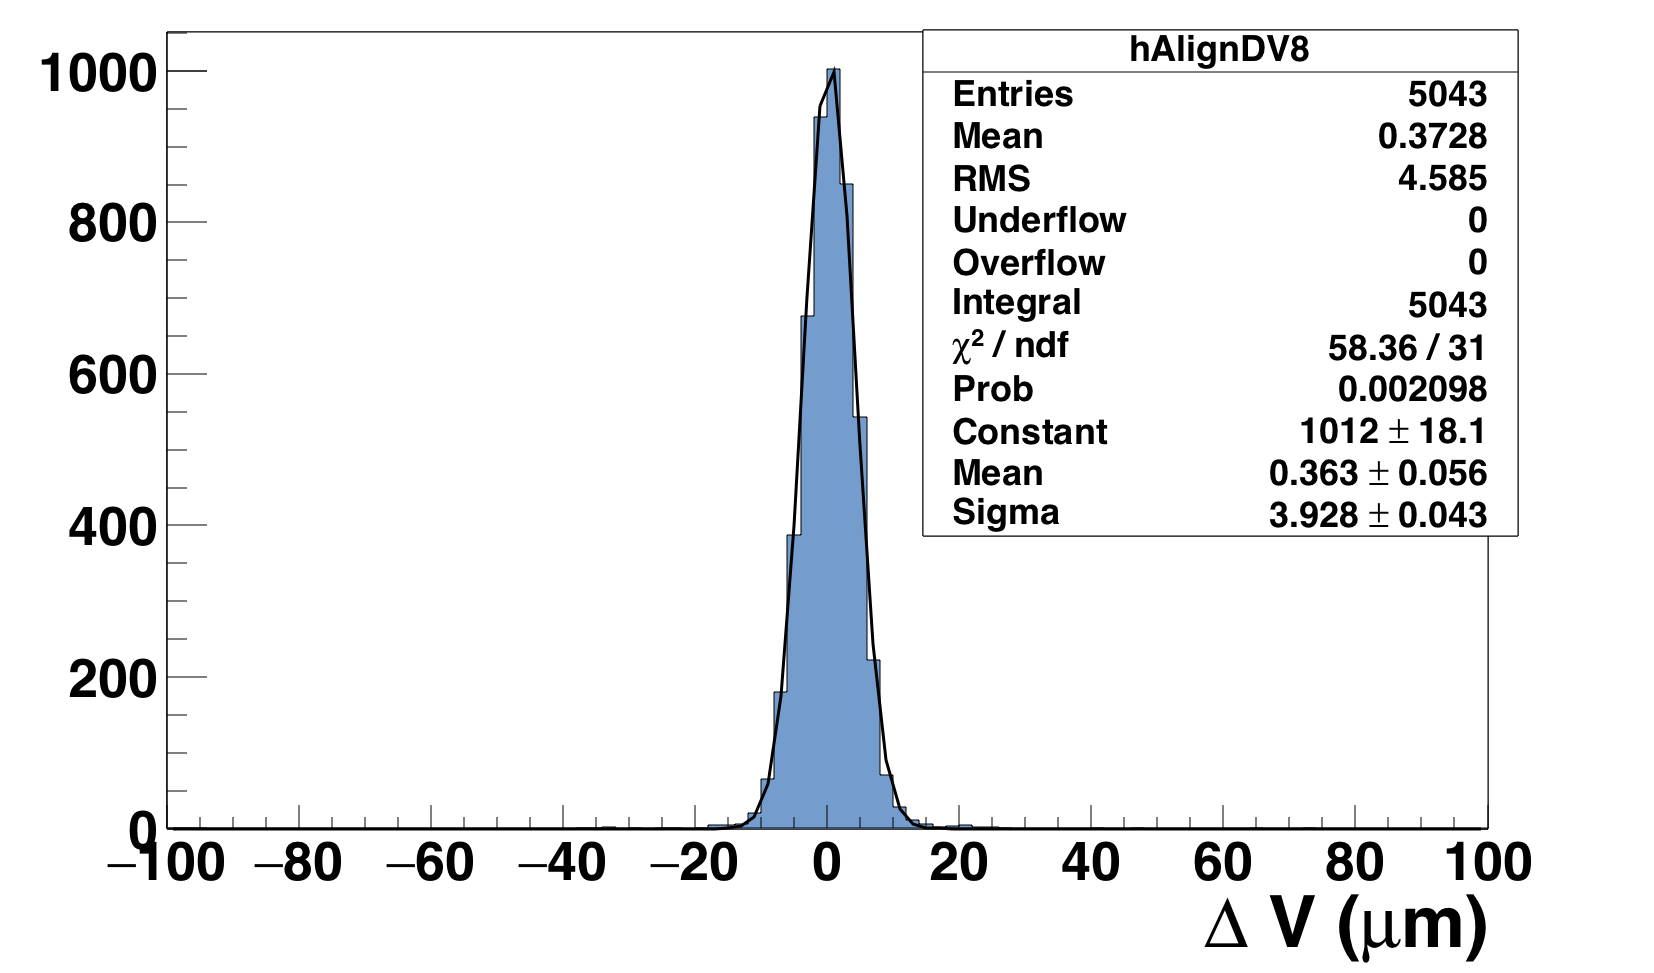
\includegraphics[width = 1.2\textwidth]{Pictures/deformation/deltaV_8_deformed.png}
          \caption{}
          \label{fig:residualVDef}
        \end{subfigure}
        \caption{Distribution of the residuals obtained for the front sensor with a tilt of $36^{\degree}$: \ref{fig:scatterDUV_deformed} $\Delta u = f(v_{hit})$, 
        \ref{fig:scatterDVU_deformed} $\Delta v = f(u_{hit})$, \ref{fig:scatterDUU_deformed} $\Delta u = f(u_{hit})$,
        \ref{fig:scatterDVV_deformed} $\Delta v = f(v_{hit})$, \ref{fig:residualUDef} distribution of the residual $\Delta u$ and \ref{fig:residualVDef} distribution of the residual $\Delta v$.
        }
        \label{fig:alignmentPlane8Deformed}
      \end{figure}

      \begin{figure}[!h]
        \centering
        \begin{subfigure}[t]{0.45\textwidth}
          \centering
          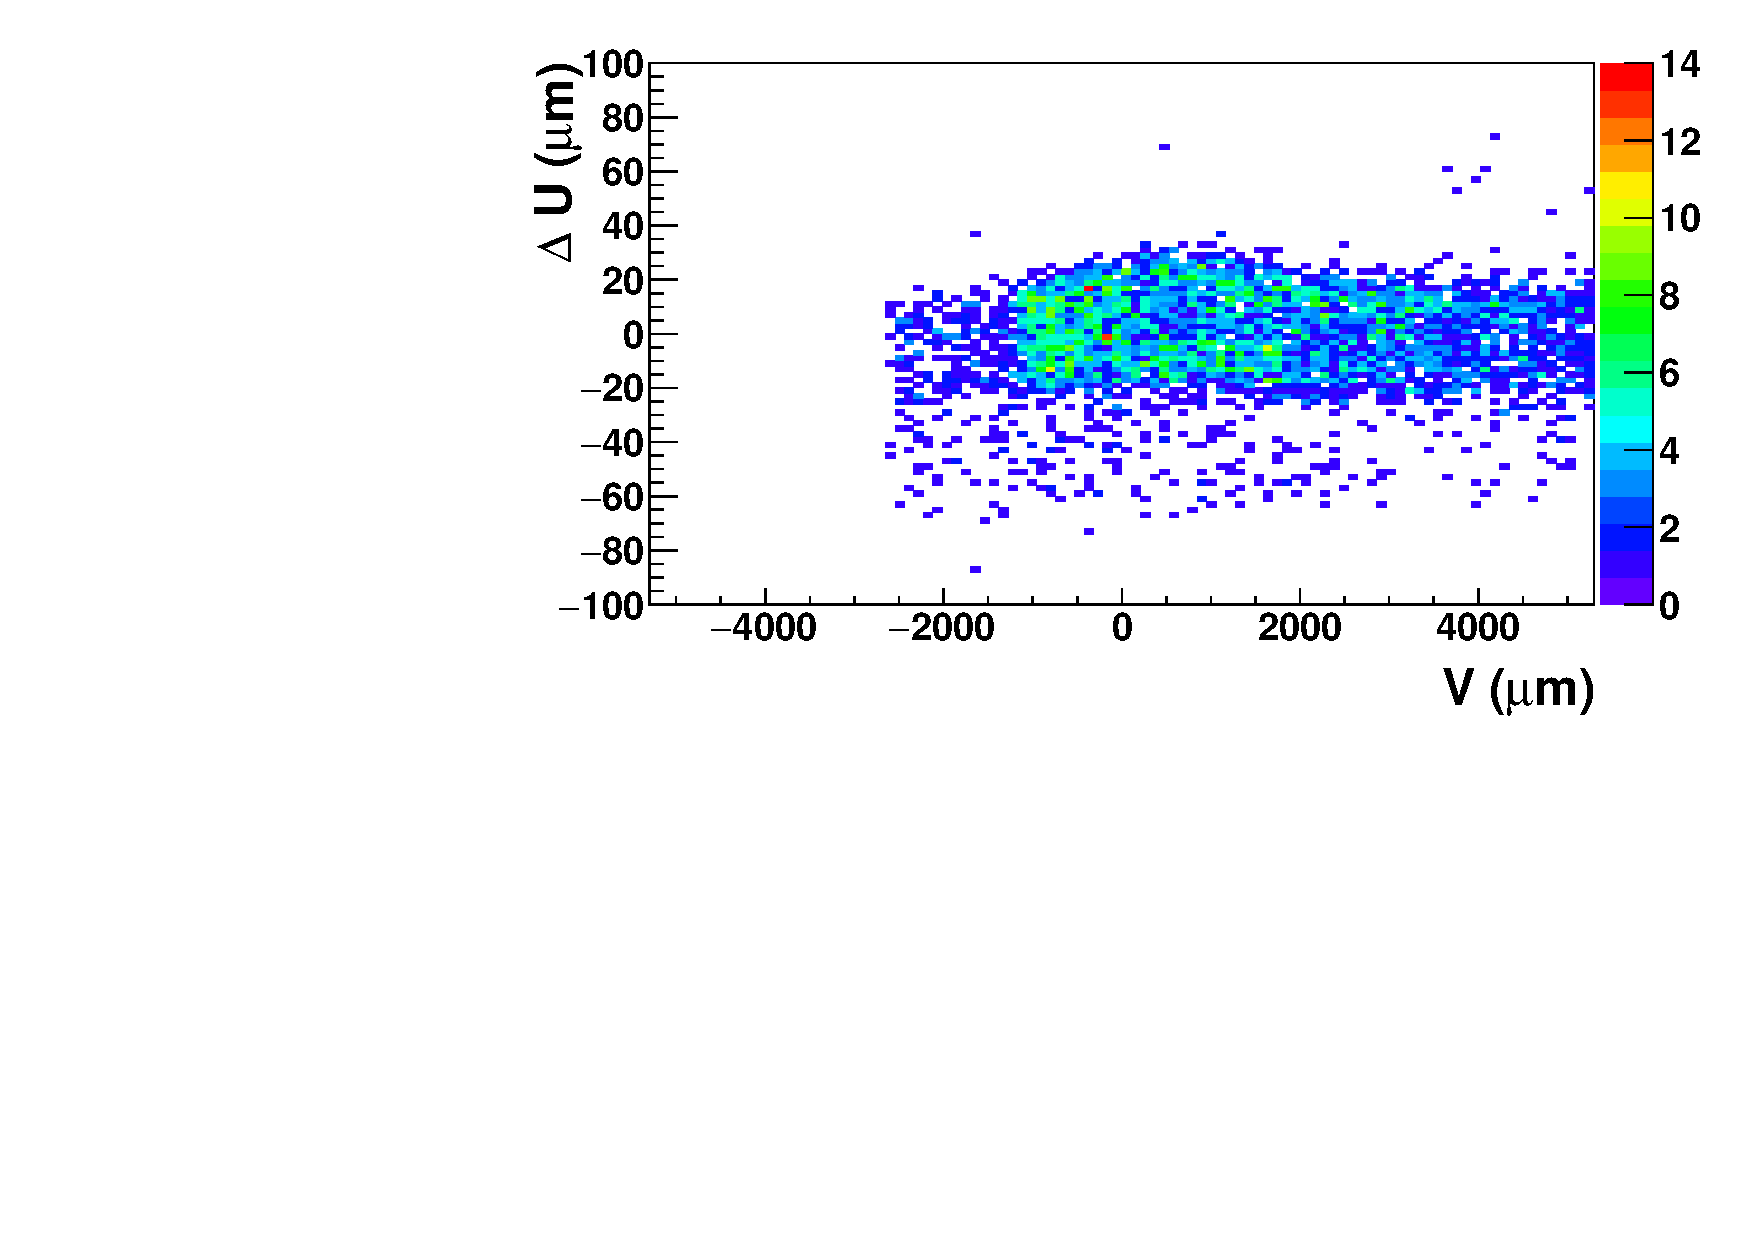
\includegraphics[width = 1.2\textwidth]{Pictures/deformation/deltaUV_6_deformed.pdf}
          \caption{}
          \label{fig:scatterDUV_deformed_back}
        \end{subfigure}
        \hfill
        \begin{subfigure}[t]{0.45\textwidth}
          \centering
          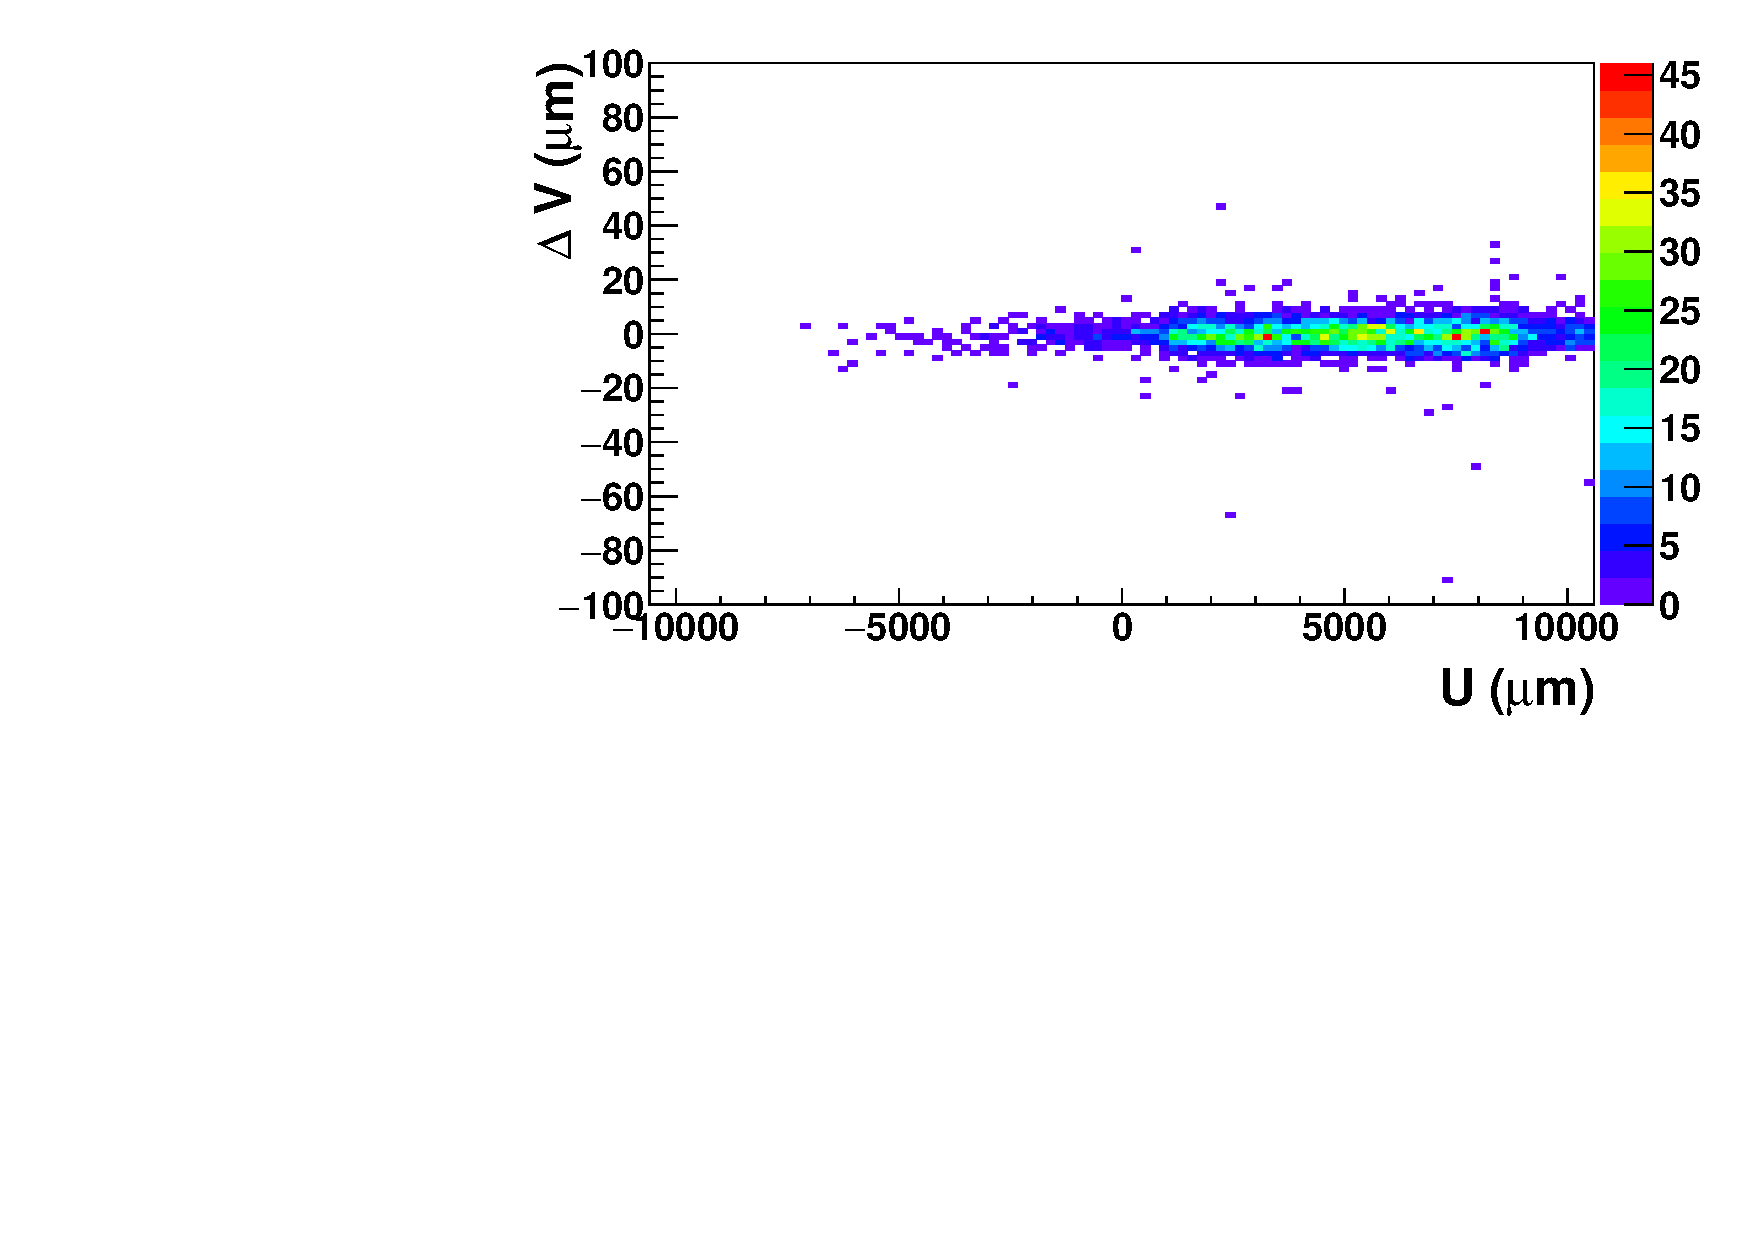
\includegraphics[width = 1.2\textwidth]{Pictures/deformation/deltaVU_6_deformed.pdf}
          \caption{}
          \label{fig:scatterDVU_deformed_back}
        \end{subfigure}

        \begin{subfigure}[t]{0.45\textwidth}
          \centering
          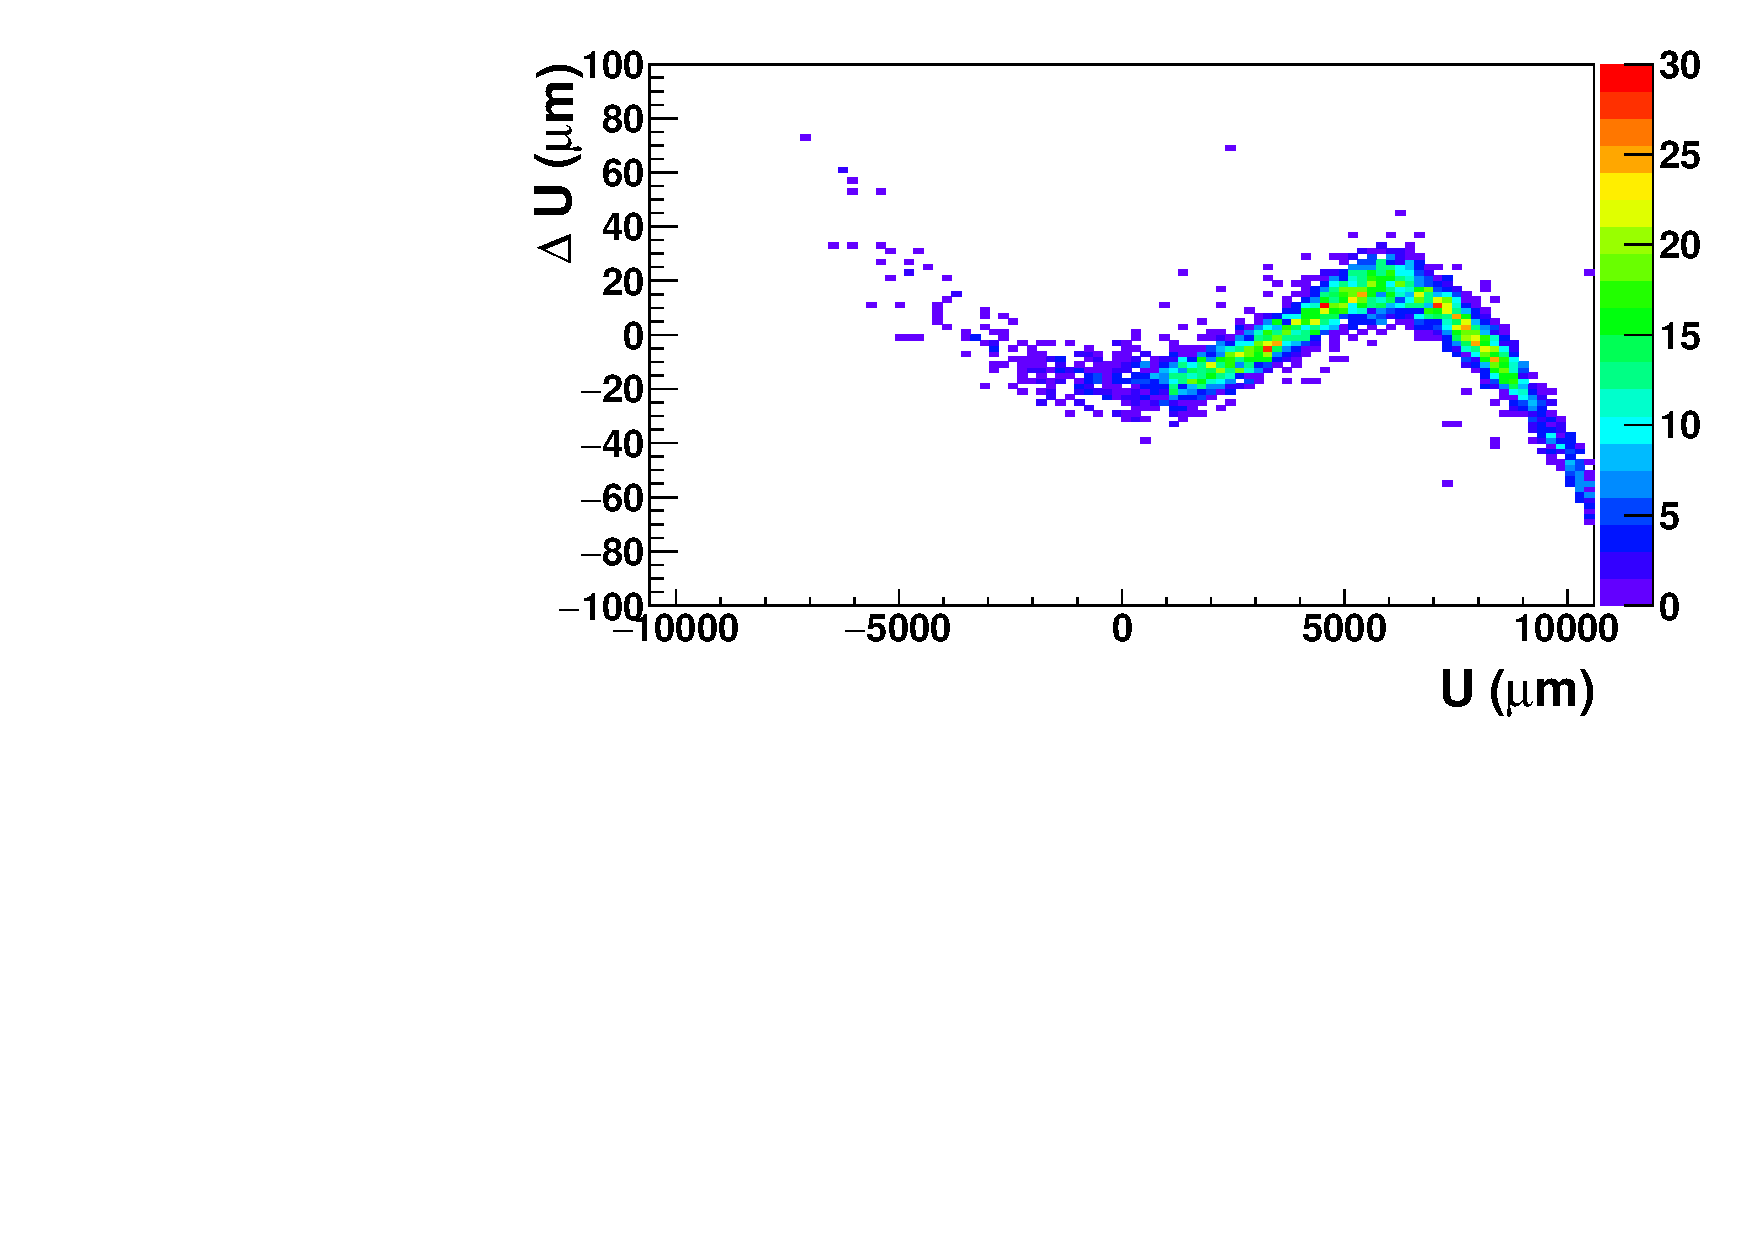
\includegraphics[width = 1.2\textwidth]{Pictures/deformation/deltaUU_6_deformed.pdf}
          \caption{}
          \label{fig:scatterDUU_deformed_back}
        \end{subfigure}
        \hfill
        \begin{subfigure}[t]{0.45\textwidth}
          \centering
          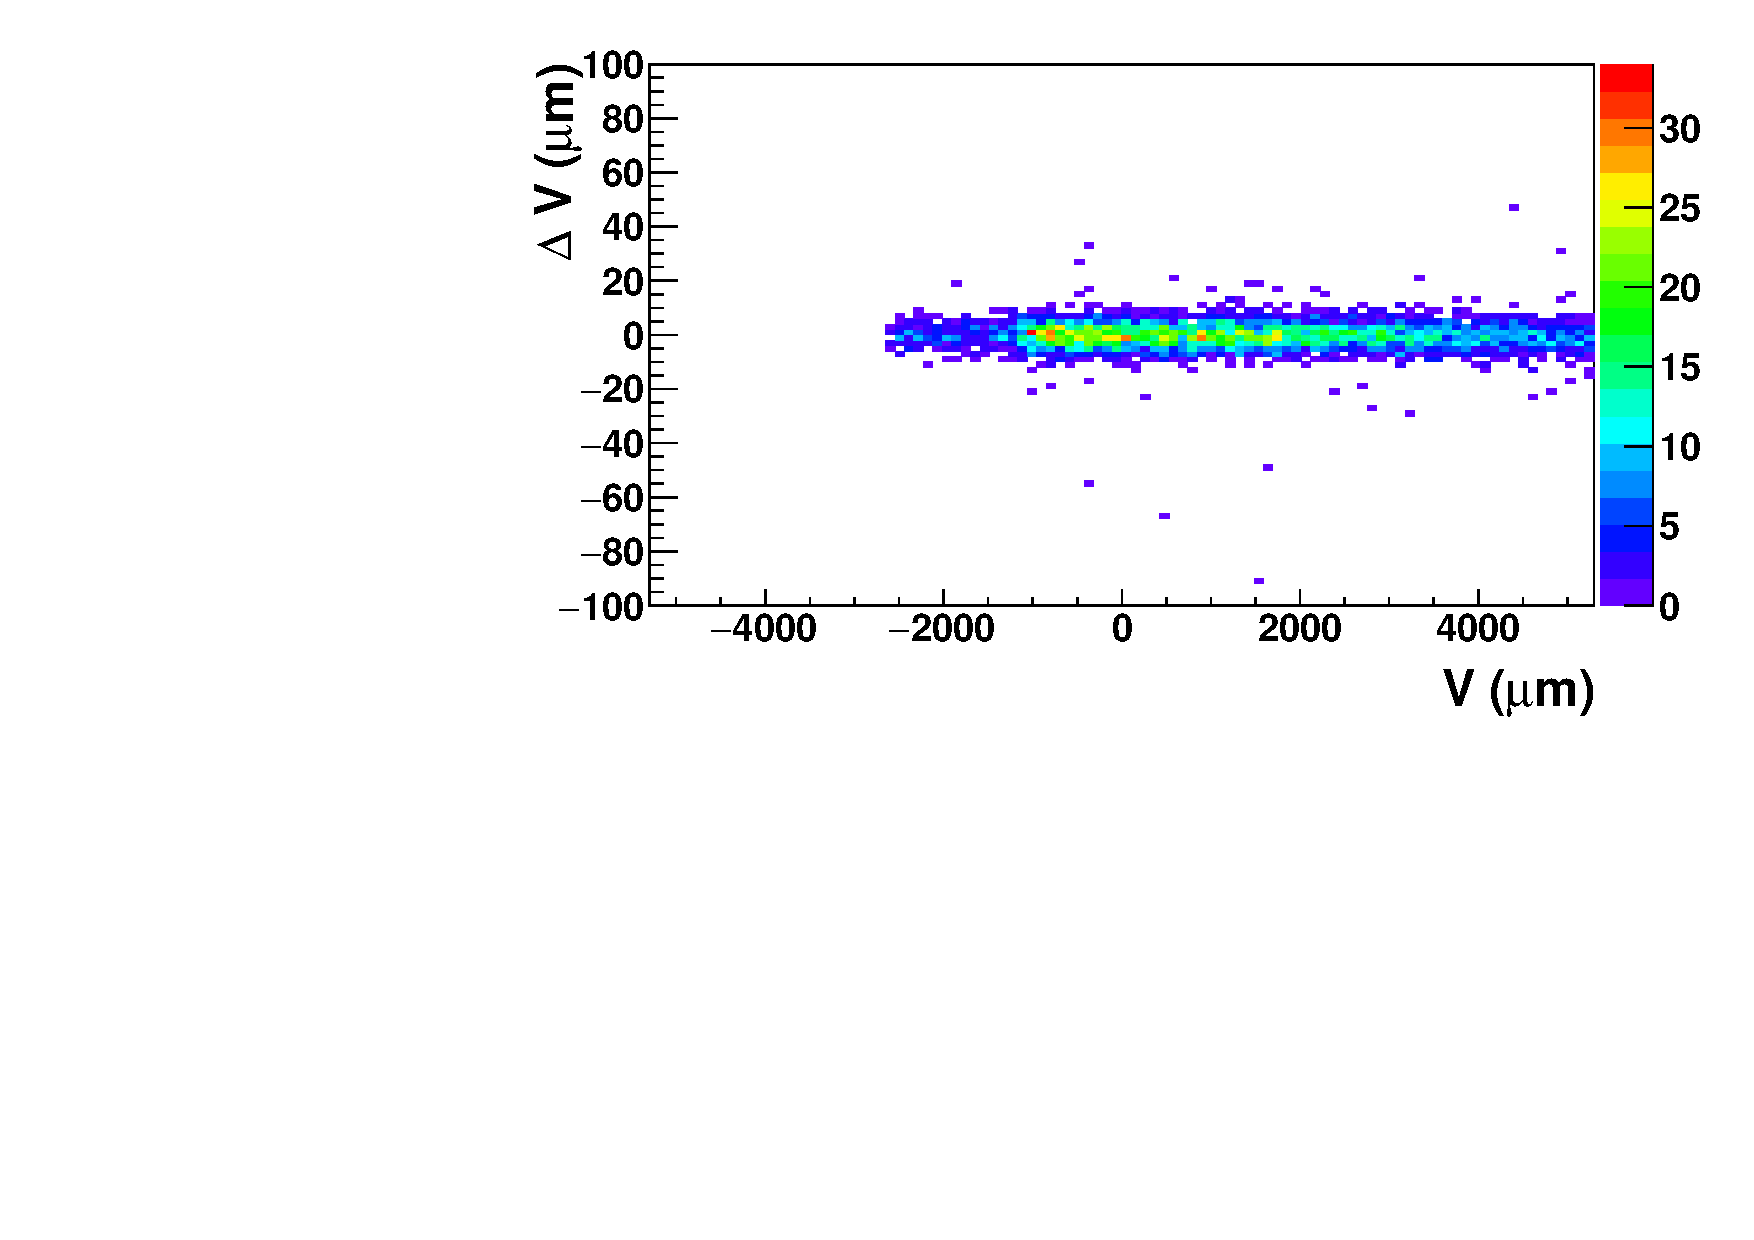
\includegraphics[width = 1.2\textwidth]{Pictures/deformation/deltaVV_6_deformed.pdf}
          \caption{}
          \label{fig:scatterDVV_deformed_back}
        \end{subfigure}

        \begin{subfigure}[t]{0.45\textwidth}
          \centering
          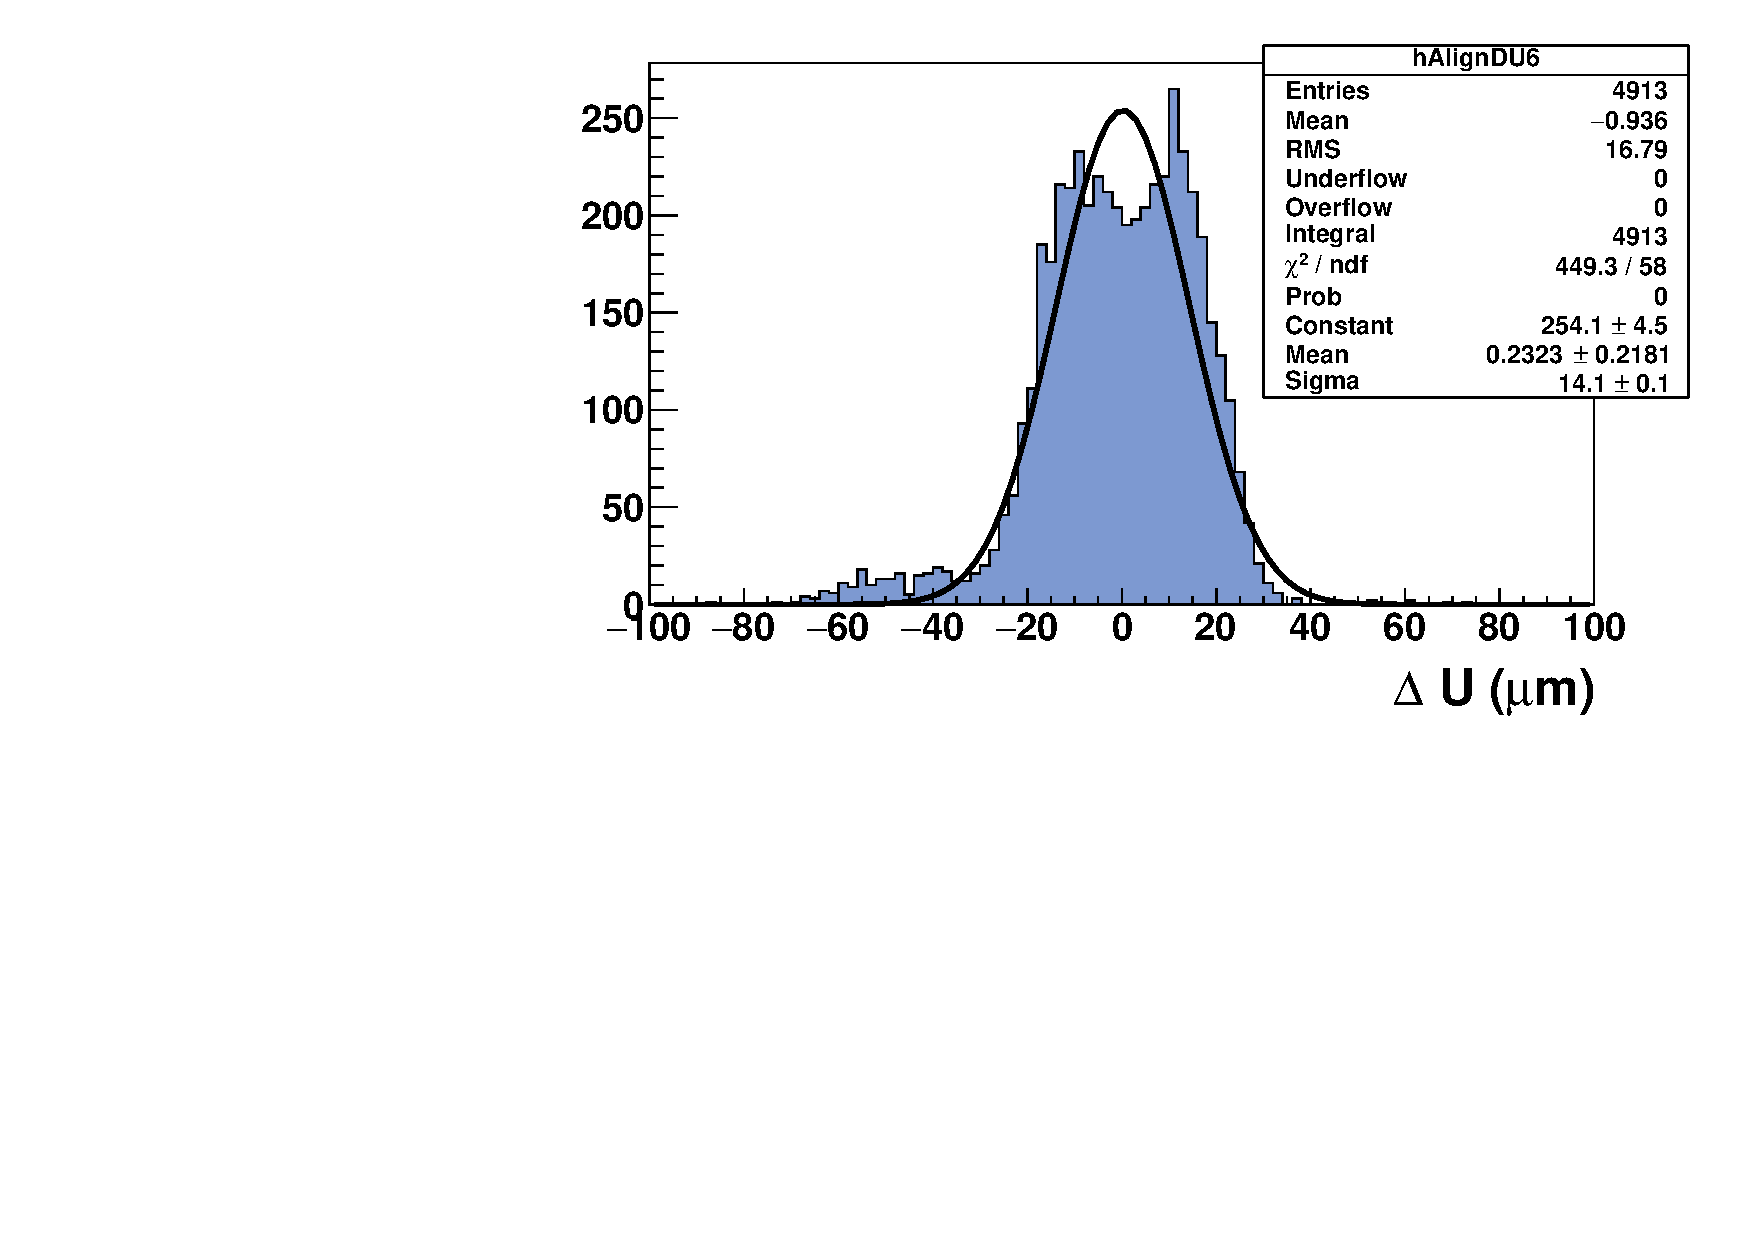
\includegraphics[width = 1.2\textwidth]{Pictures/deformation/deltaU_6_deformed.pdf}
          \caption{}
          \label{fig:residualUDef_back}
        \end{subfigure}
        \hfill
        \begin{subfigure}[t]{0.45\textwidth}
          \centering
          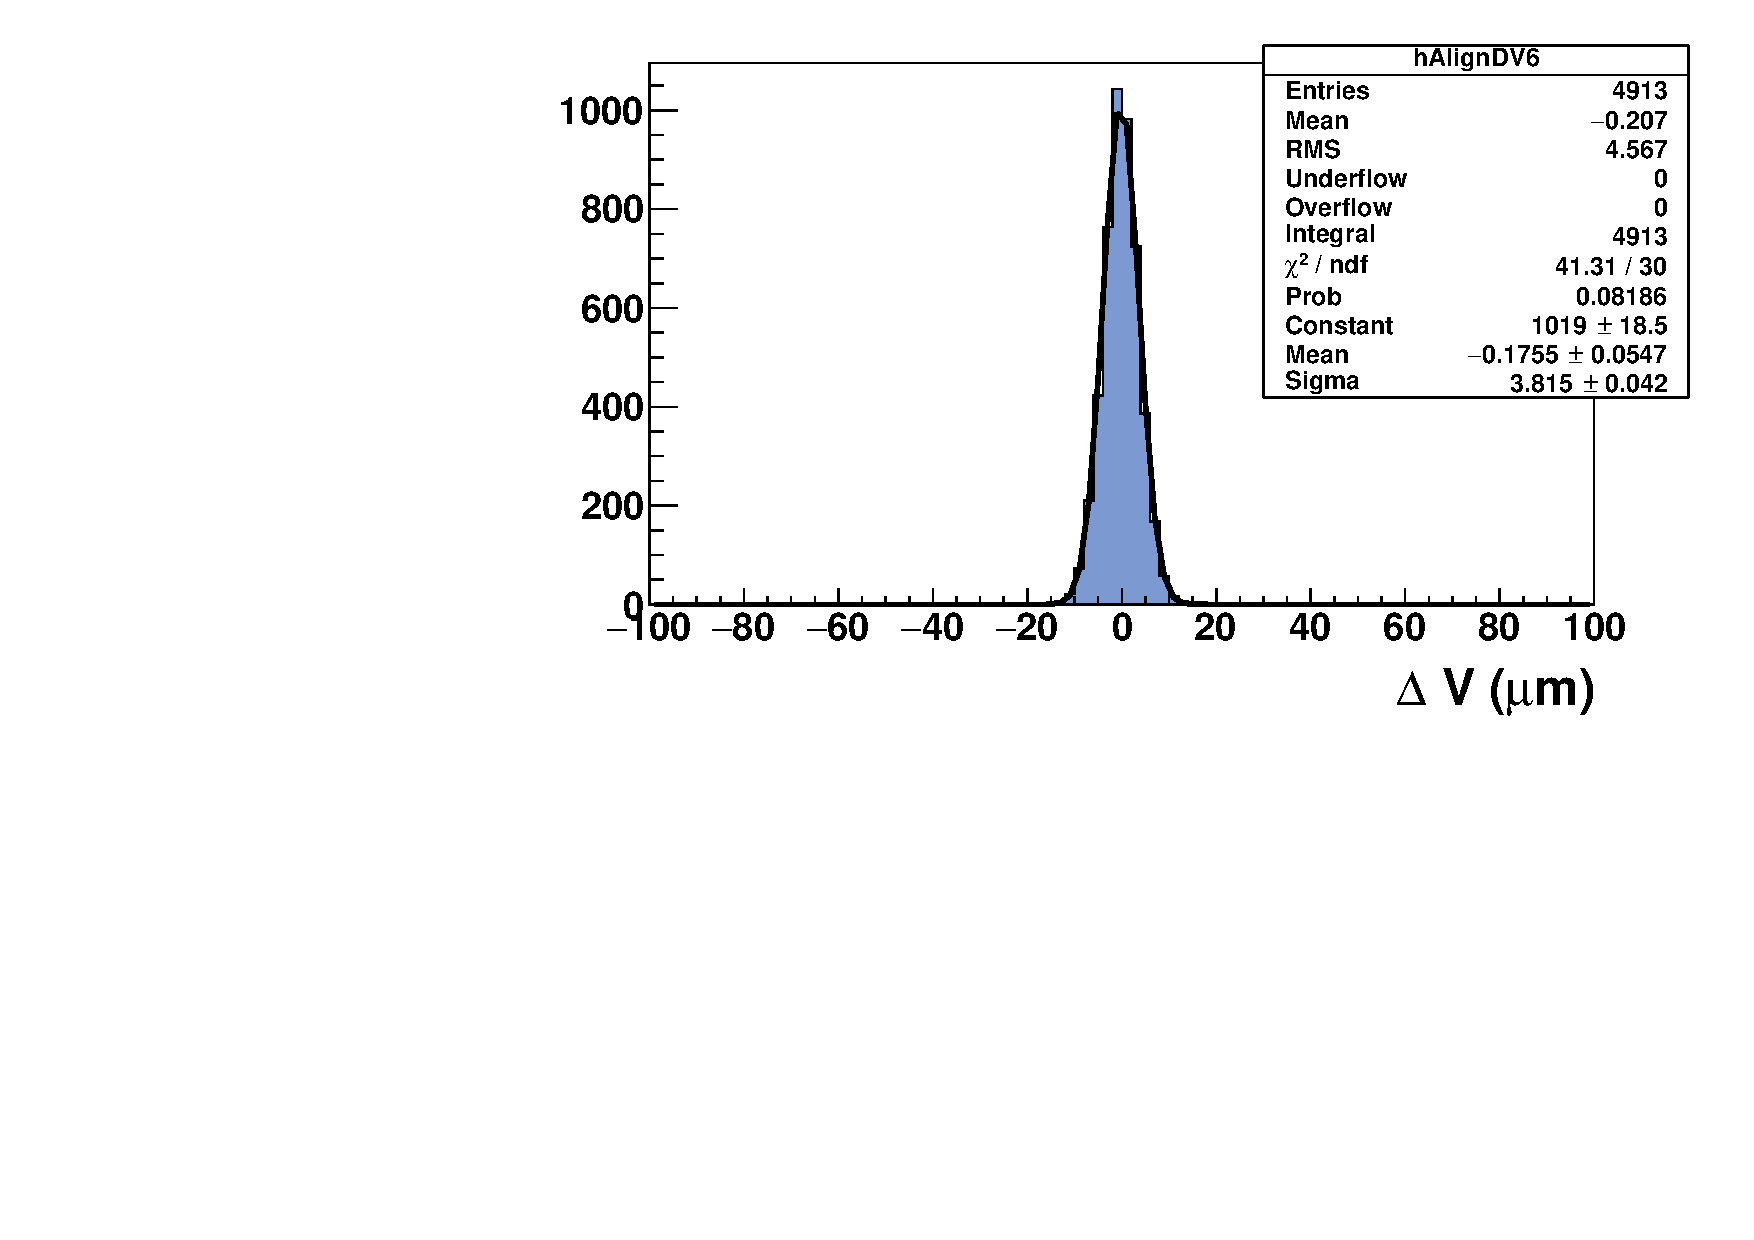
\includegraphics[width = 1.2\textwidth]{Pictures/deformation/deltaV_6_deformed.pdf}
          \caption{}
          \label{fig:residualVDef_back}
        \end{subfigure}
        \caption{Distribution of the residuals obtained for the back sensor with a tilt of $36^{\degree}$: \ref{fig:scatterDUV_deformed_back} $\Delta u = f(v_{hit})$, 
        \ref{fig:scatterDVU_deformed_back} $\Delta v = f(u_{hit})$, \ref{fig:scatterDUU_deformed_back} $\Delta u = f(u_{hit})$,
        \ref{fig:scatterDVV_deformed_back} $\Delta v = f(v_{hit})$, \ref{fig:residualUDef_back} distribution of the residual $\Delta u$ and \ref{fig:residualVDef_back} distribution of the residual $\Delta v$.
        }
        \label{fig:alignmentPlane8Deformed_back}
      \end{figure}

      \subsubsection{Origin of the deviations}

      The deviations observed are mainly caused by the characteristics of the ladder.
      Ultra-thin sensors with a thickness of approximately $50 \text{ }\mu\text{m}$ are used.
      Naturally, without any mechanical structure, the sensors tend to be very flexible and not self-supporting.
      Nevertheless, the gluing procedure to the flex-cable and the \gls{SiC} foam induces permanent deformations of the surface that can not be flattened.
      Also, the foam has an open-cell structure with small bumps and the glue spots might be more or less important on some positions.
      The Bristol group has performed a mechanical survey on a mechanical prototype, which has non-functioning MIMOSA-20 sensors.
      The chips were thinned and attached to the standard flex-circuits.
      The measurements done with an optical survey equipment have revealed a peak-to-peak flatness of the order of the $100 \text{ }\mu\text{m}$ on both sides.
      Figure~\ref{fig:mechanicalSurvey} shows the result of this survey.
      The overall shape is due to the intrinsic shape of the foam.
       
      \begin{figure}[!h]
        \centering
        \begin{subfigure}[t]{0.45\textwidth}
          \centering
          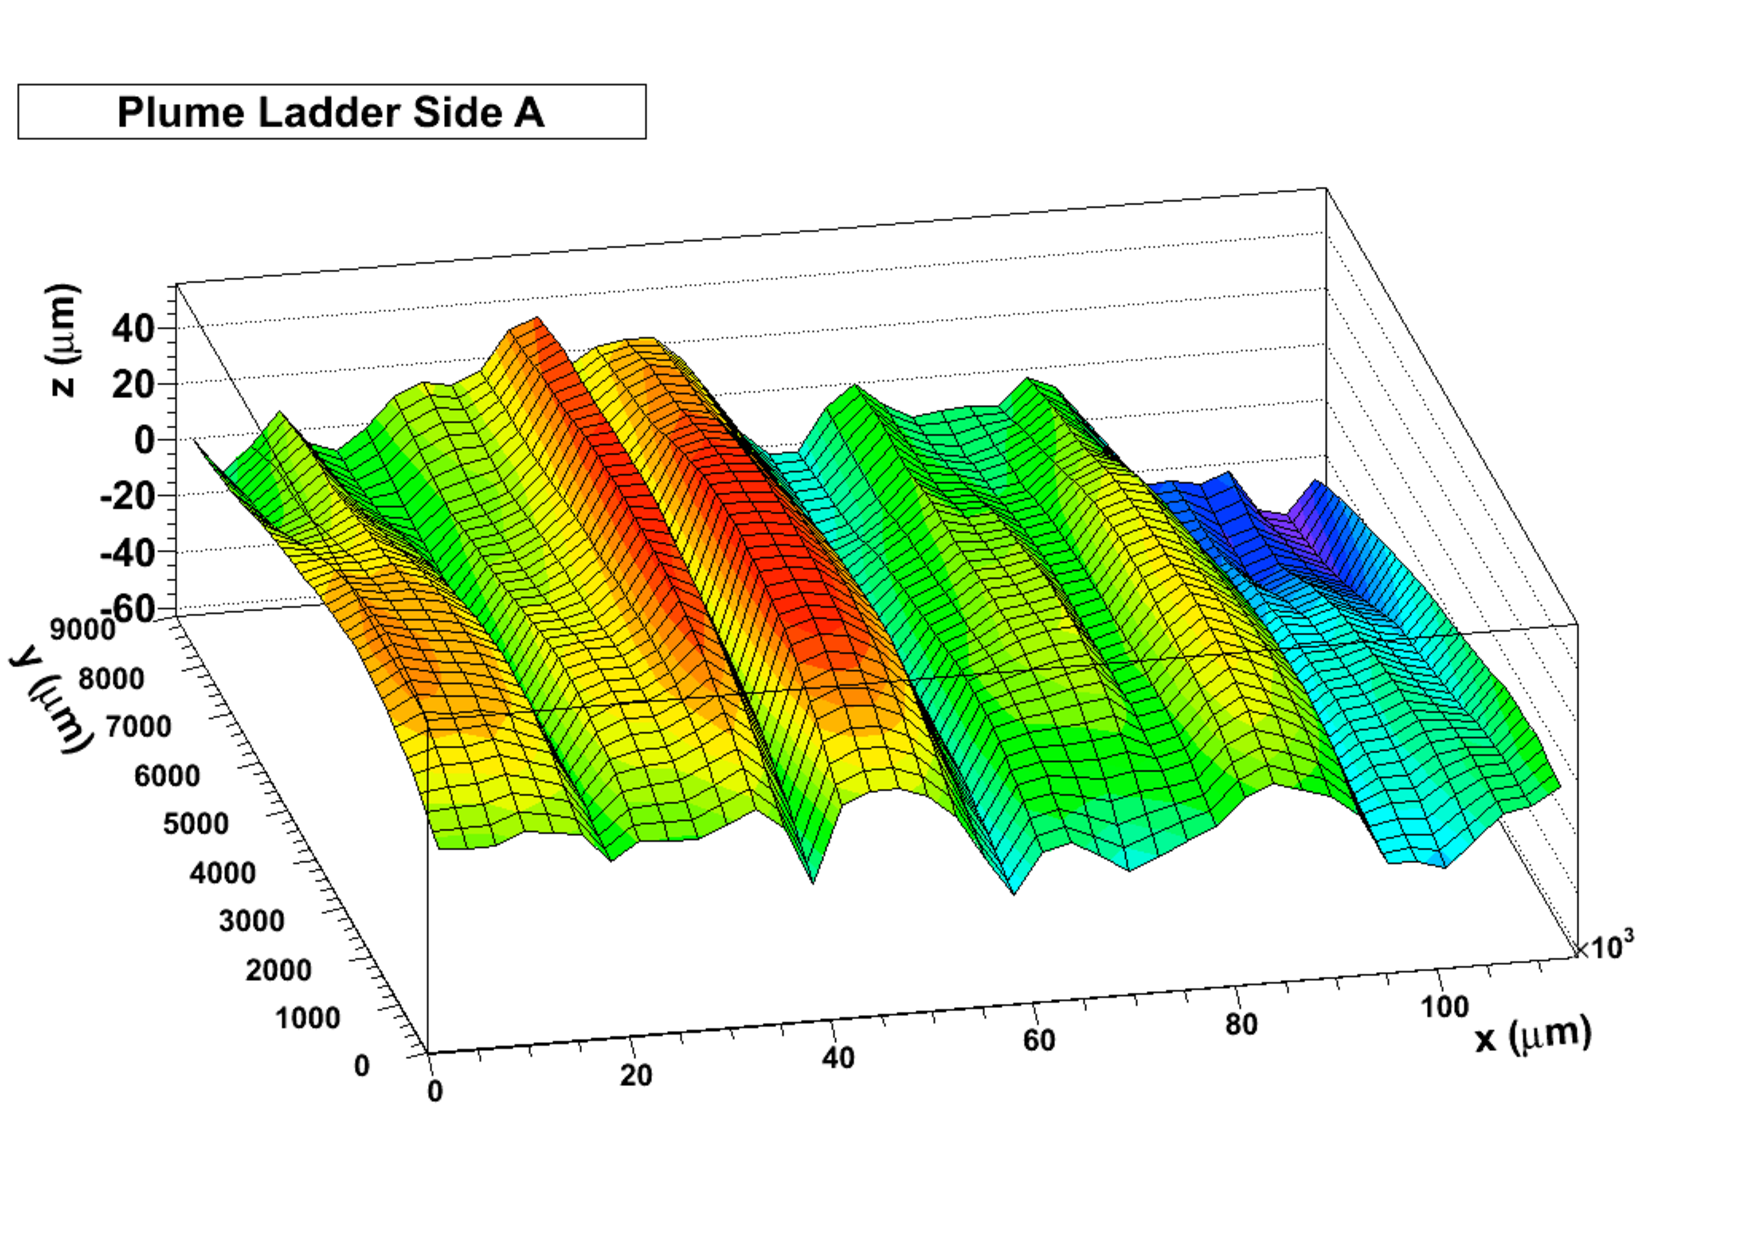
\includegraphics[width = 1.2\textwidth]{Pictures/deformation/surveyResults.pdf}
        \end{subfigure}
        \hfill
         %add desired spacing between images, e. g. ~, \quad, \qquad, \hfill etc. 
          %(or a blank line to force the subfigure onto a new line)
        \begin{subfigure}[t]{0.45\textwidth}
          \centering
          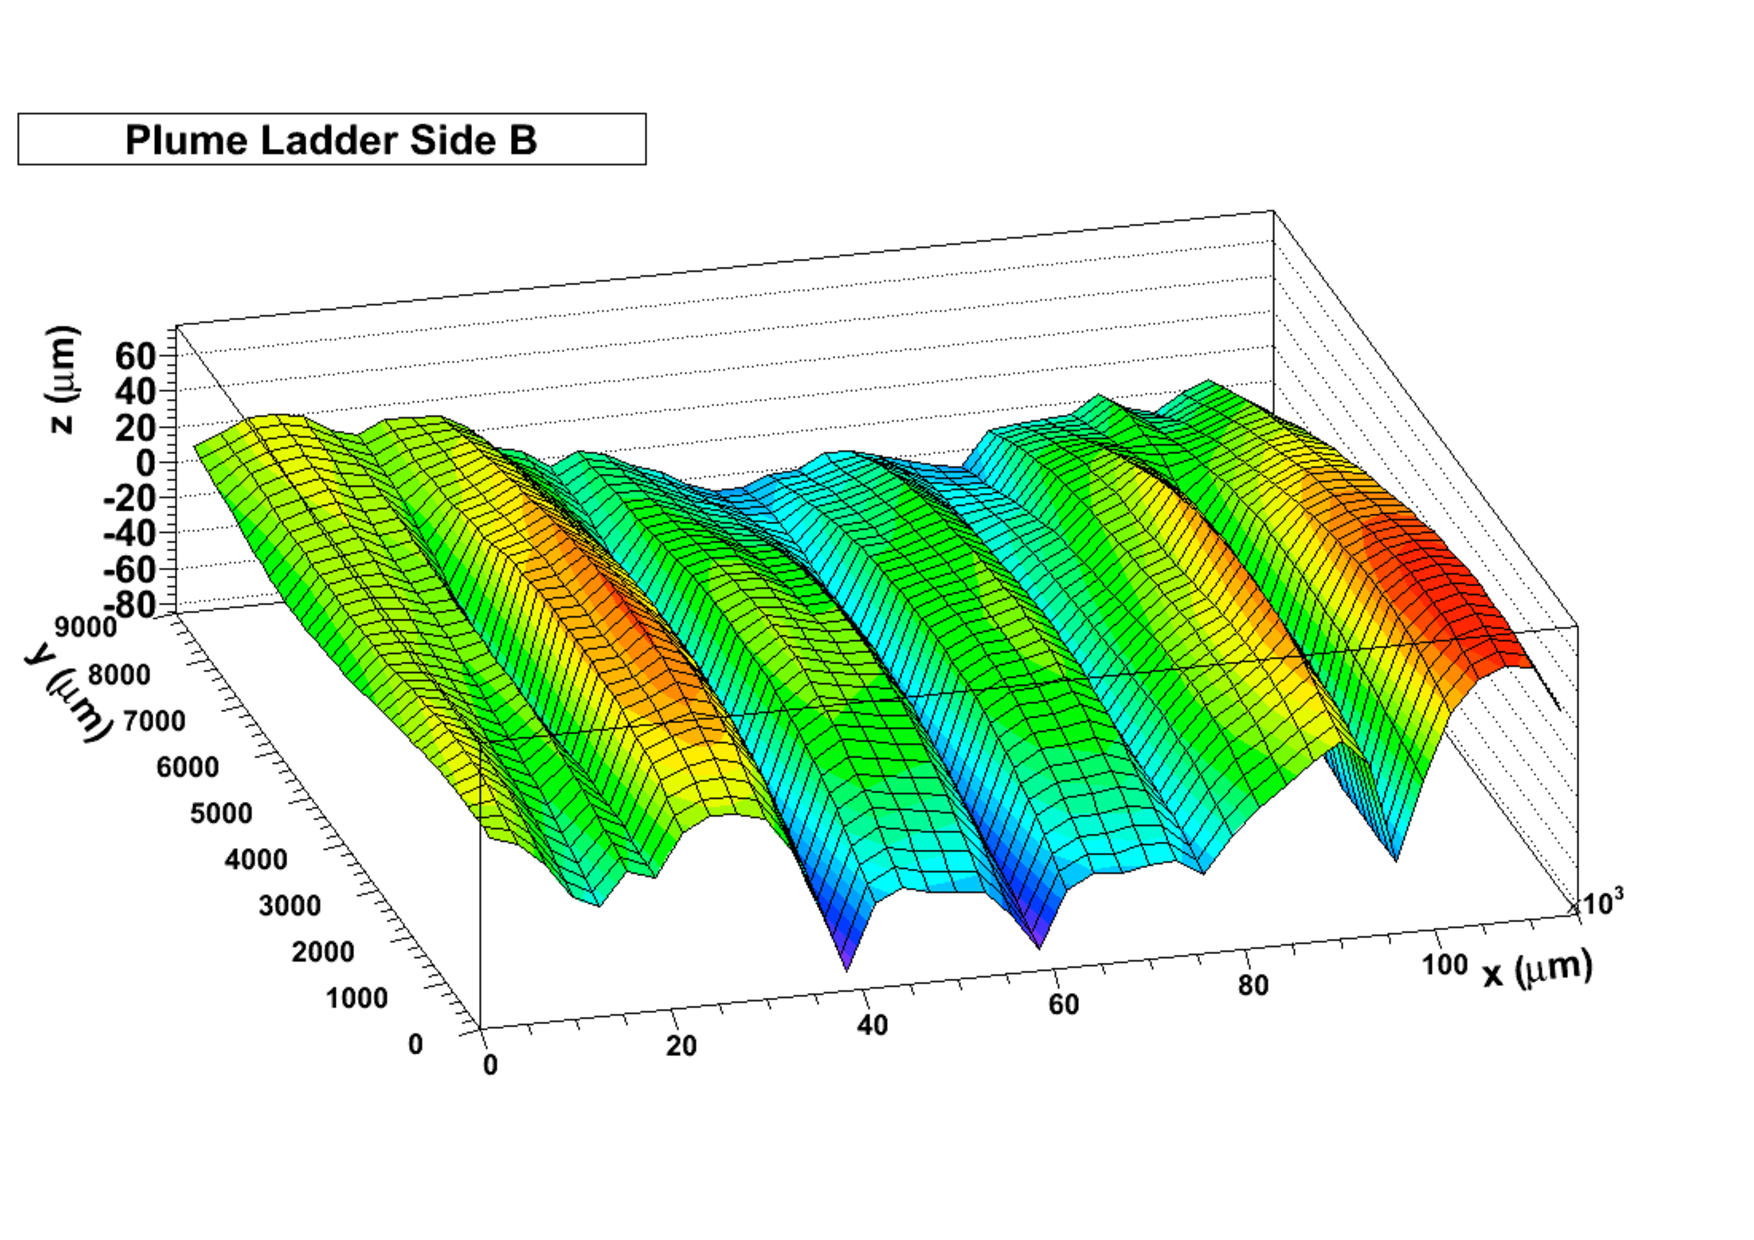
\includegraphics[width = 1.2\textwidth]{Pictures/deformation/surveyResultsB.pdf}
        \end{subfigure}

        \caption{Results of the mechanical survey of each side of the PLUME mechanical prototype.}
        \label{fig:mechanicalSurvey}
      \end{figure}

      Another parameter has to be taken into account to explain the deviation observed.
      During the analysis, this non-flatness structure is not taken into account.
      The sensors are modelled as completely flat planes and the $z$-position is fixed.
      However, the sensor's position in three dimensions is actually different due to the deformations.
      When the particles are not striking the sensor in normal incidence, the hit predicted with respect to the flat plane does not have the same position anymore.
      Thus, the residual between the position of the extrapolated track and the predicted hit is increasing.
      Figure~\ref{fig:originDef} depicts the difference between the hit expected $U_{h}$ on the flat plane and the extrapolation of the actual hit $U'_{\text{h extrapolated}}$.
      For a normal incidence, these two hits are at the same position, but larger is the angle, larger is the difference between the expected hit and the extrapolated one.
      The deformation height $\delta w$ can be expressed as a function of the angle $\theta$ and the residual $\delta u$ of the track:

      \begin{equation}
        \delta w = \frac{\delta u}{\tan(\theta)}
        \label{eq:deltaW}
      \end{equation}

      Thus, the visible deformation of the surface is sensitive to the angle of the incoming track.
      In the case presented above, the angle of the incoming track is only in one direction and so, the deformations are visible only in the $u$-direction and the other one is not affected, even if the deformations are in two dimensions.

      \begin{figure}[!h]
      \centering
        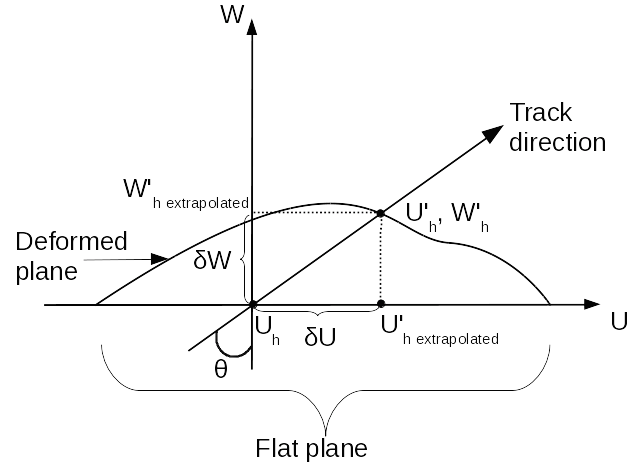
\includegraphics[width = 0.8\textwidth]{Pictures/deformation/origin_deformation.png}
        \caption{Side view of the sensor's deformation.}
        \label{fig:originDef}
      \end{figure}

      \subsubsection{Algorithm to estimate the deformations}

      The sensor deformations were already studied in Strasbourg by Maria Robert Daniel.
      The sensor was mapped for the alignment in order to remove the contribution of the deviation on the residual \cite{maria}.
      As this method is done manually and is time-consuming, an automatic method has to be implemented.
      A similar effect was observed in the CMS tracker during the alignment procedure with cosmic rays and a method was developed to compensate the deformations \cite{CMSalignment}. 
      They have used modified two-dimensions Legendre polynomials to parametrise the sensors' deformations and therefore, they were able to minimise the effect of the deviations during the alignment procedure of the tracker.
      The method implemented in TAF was inspired by the work which was done by the CMS collaboration.
      Nonetheless, contrary to the CMS tracker, the tilt was produced only in one direction.
      Hence, the two-dimensions Legendre polynomials can not be used to parametrise the sensor's deformations, but the problem is still the same.
      Tracks with a large angle of incidence are more sensitive to the exact position of the plane in three dimensions, so the coordinates of the hits have to be exactly known.
      The deviations observed on figure~\ref{fig:scatterDUU_deformed} provide an information on the behaviour of the deformation, that is extrapolated to the position of the plane on the $w$-direction.
      Thus, the hit position is calculated again with respect to the sensor's surface shape extrapolated.
      This shape is guessed from the track-hit residuals as a function of the hit position in the same direction.
      A Legendre function is used to fit the curve and the coefficient given by the fit steps are used to calculate the deformation of the plane.
      The equation~\ref{eq:polynomials} represents the extrapolated shape of the plane in the $w$-direction calculated with respect to the expected hit position $u_{r}$, which is normalised to the sensor width.

      \begin{equation}
        w\left(u_{r}\right) = \sum_{k=0}^n \omega_{k}P_{k}\left(u_{r}\right)
        \label{eq:polynomials}
      \end{equation}
      
      The $\omega_{k}$ are the coefficients that quantify the sensor curvature and $P_{k}(u_{r})$ are the Legendre polynomials defined by the equation~\ref{eq:Legendre}:

      \begin{equation}
        P_{k}\left(u_{r}\right) = \frac{1}{2^{k}!}\frac{d^{k}}{du_{r}^{k}} \left( (u_{r}^2 - 1)^{k}\right)
        \label{eq:Legendre}
      \end{equation}

      Then, the exact hit position is calculated by correcting the hit position extrapolated by $\left(-\omega(u_{r}).\tan{\theta}\right)$, according to the equation~\ref{eq:deltaW} and the residual $\Delta u$ is determined by taking into account the tracks' angle during the analysis.      

      \begin{figure}[h]
        \centering
        \begin{subfigure}[t]{0.45\textwidth}
          \centering
          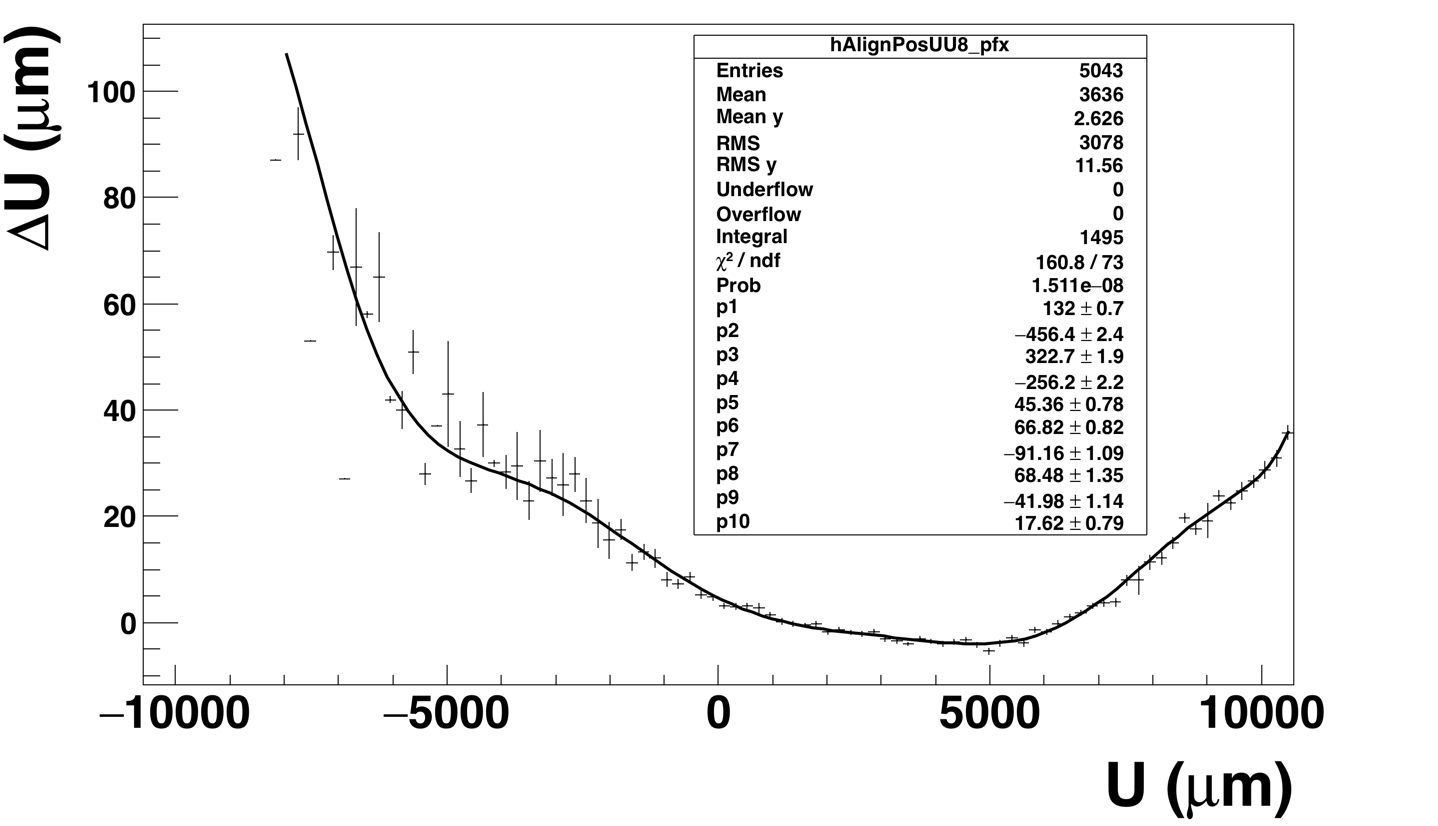
\includegraphics[width = 1.2\textwidth]{Pictures/deformation/profileFitted_pl8.png}
          \caption{}
          \label{fig:profileFitted_front}
        \end{subfigure}
        \hfill
        \begin{subfigure}[t]{0.45\textwidth}
          \centering
          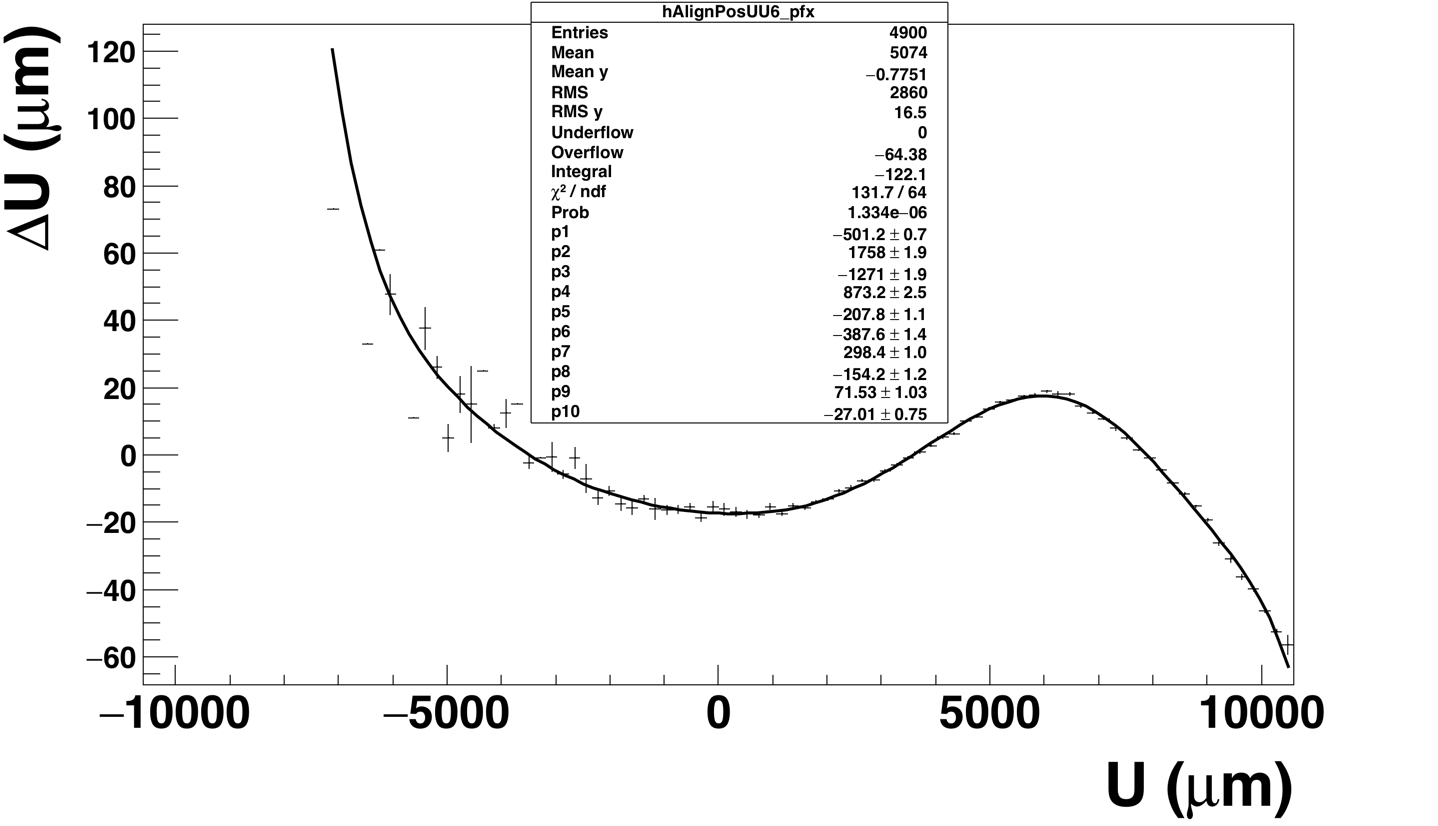
\includegraphics[width = 1.2\textwidth]{Pictures/deformation/profileFitted_pl6.png}
          \caption{}
          \label{fig:profileFitted_back}
        \end{subfigure}
        \caption{Profile of the scatter plot showing the track-hit residual in the $u$-direction as a function of the hit position on the plane for the same direction: \ref{fig:profileFitted_front} is the profile of the front plane and \ref{fig:profileFitted_back} is the profile of the back plane.
        Both profiles were fitted with a sum of Legendre polynomials up to the eleventh order.} 
        \label{fig:profileFitted}
      \end{figure}

      \subsubsection{Correction of the deformation}

      Contrary to the CMS case, the Legendre polynomials used here are calculated in one dimension as the tilt is only in one direction.
      The scatter plot displayed in subsection~\ref{subsec:deformation} was profiled and fitted with a Legendre function.
      The sum of Legendre polynomials up to different orders was tried to find the function fitting the best the profile.
      The coefficients obtained after fitting are used to parametrise the surface's shape and the position of the hit.
      Table~\ref{tab:chi2} summarises the different $\chi^2 \text{/NDF}$ obtained for the different orders, as well as the residual measured in the $u$-direction after correction.

      \begin{table}[!h]
        \centering
        \begin{tabular}{c c c c c}
          \hline %----------------------------
           & \multicolumn{2}{ c }{Front plane} & \multicolumn{2}{ c }{Back plane} \tabularnewline
          \hline %----------------------------
          Order & $\chi^2 \text{/NDF}$ & $\sigma_{U}^{front}$ & $\chi^2 \text{/NDF}$ & $\sigma_{U}^{back}$ \tabularnewline
          \hline %----------------------------
          \hline %----------------------------
          3 & 21683.9/84 & 6.508 & 35575.2/72 & 13.28 \tabularnewline
          4 & 1449.91/83 & 6.176 & 25129.8/71 & 12.38 \tabularnewline
          5 & 1449.79/82 & 5.998 & 1718.81/70 & 6.918 \tabularnewline
          6 & 653.738/81 & 5.924 & 1480.55/69 & 6.817 \tabularnewline
          7 & 304.206/80 & 5.922 & 634.696/68 & 6.406 \tabularnewline
          8 & 288.376/79 & 5.937 & 269.296/67 & 6.228 \tabularnewline
          9 & 225.376/78 & 5.9 & 250.565/66 & 6.239 \tabularnewline
          10 & 225.353/77 & 5.914 & 152.236/65 & 6.159 \tabularnewline
          11 & 158.053/76 & 5.913 & 131.727/64 & 6.176 \tabularnewline
          \hline %----------------------------
         \end{tabular}
         \caption{Fit results of the scatter plot $\Delta U = f(U)$ for Legendre polynomials order and the residual obtained on each side of the PLUME ladder.}
         \label{tab:chi2}
      \end{table}
 
      A second-order Legendre function does not fit well the profile of $\Delta U=f(u_{hit})$ and does not provide a good improvement on the compensation of deformation.
      The best improvement was achieved on both sides from the $8^{th}$ order Legendre polynomials to higher values.
      Although the $\chi^2 \text{/NDF}$ is better for higher order, the width of the residual distribution is of the same order ($\sigma_{front}\simeq 5.9 \text{ }\mu\text{m}$ and $\sigma_{back} \simeq 6.2 \text{ }\mu\text{m}$).
      Figure~\ref{fig:profileFitted_front} depicts the fit results for the front plane ans figure~\ref{fig:profileFitted_back} is for the back plane.
      For both figures, the deviation is not well fitted for the negative values.
      The dispersion of the residuals is wider. 

      For example, using a $11^{th}$ order Legendre polynomials has improved the spatial residual for both planes. 
      Instead of $\sigma_{u} \simeq 6.8 \text{ }\mu\text{m}$ for the front plane, the spatial residual is $\sigma_{u} \simeq 5.9 \text{ }\mu\text{m}$, namely an improvement of 13.2 \% of the measured spatial residual and achieving a pointing resolution of $5.6 \text{ }\mu\text{m}$ for a tilt at $36^{\degree}$.
      Concerning the back plane, the spatial residual measured was $14.1 \text{ }\mu\text{m}$ and after the correction it achieves $6.2 \text{ }\mu\text{m}$, namely an improvement of 56.0 \% on the measured spatial residual.
      The point resolution of the plane is then $5.9 \text{ }\mu\text{m}$
      As it can be seen on figure~\ref{fig:scatterDUU_corrected_front}, the deviations are reduced. 
      Nevertheless, the edges of the plot are less corrected.
      This is due to the fact that the length of the sensor used to parametrise the Legendre function is a bit different to the real size of the sensor due to the deformation.
      On the back plane, a bump is still visible in the middle of the scatter plot (see figure~\ref{fig:scatterDUU_corrected_back}).
      This may be due to a missing information on the deformation of the sensor in the other direction.

      \begin{figure}[!h]
        \centering
        \begin{subfigure}[t]{0.45\textwidth}
        \centering
          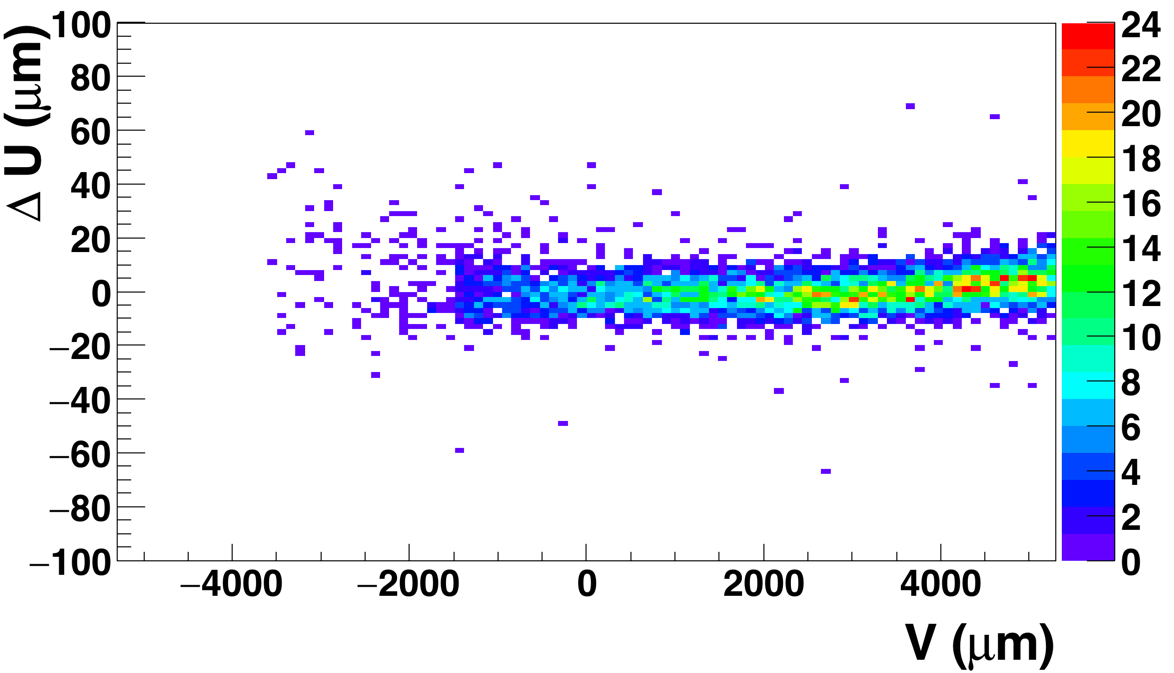
\includegraphics[width = 1.2\textwidth]{Pictures/deformation/deltaUV_8_corrected1.png}
          \caption{}
          \label{fig:scatterDUV_corrected_front}
        \end{subfigure}
        \hfill
        \begin{subfigure}[t]{0.45\textwidth}
          \centering
          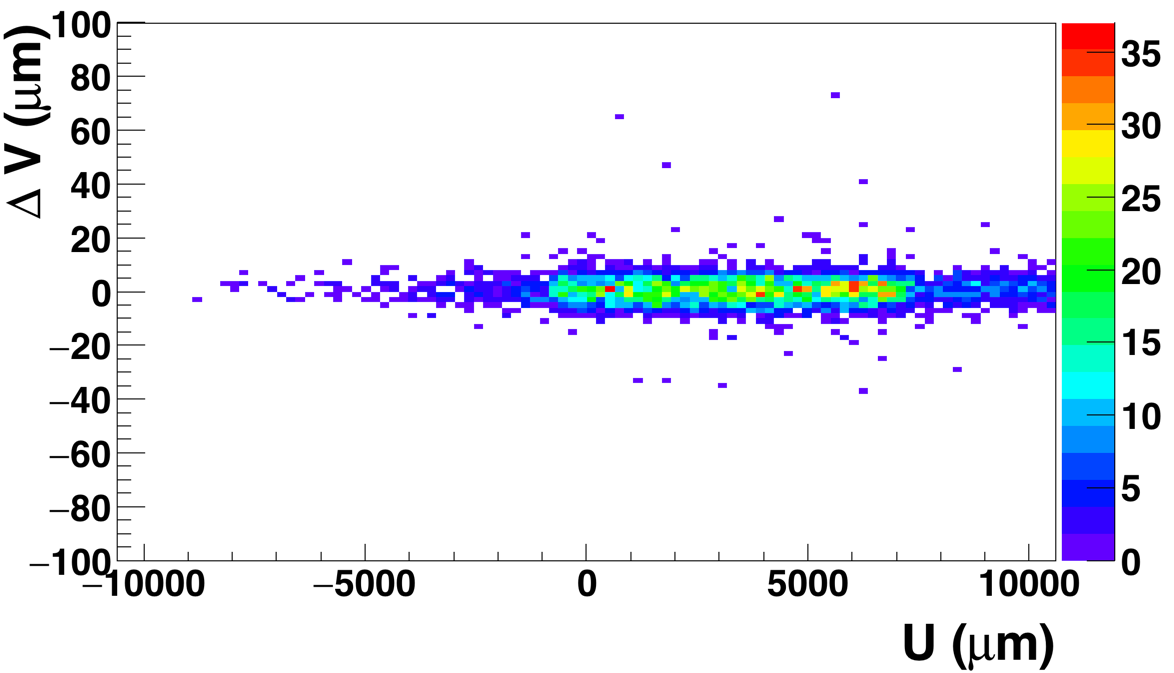
\includegraphics[width = 1.2\textwidth]{Pictures/deformation/deltaVU_8_corrected1.png}
          \caption{}
          \label{fig:scatterDVU_corrected}
        \end{subfigure}

        \begin{subfigure}[t]{0.45\textwidth}
          \centering
          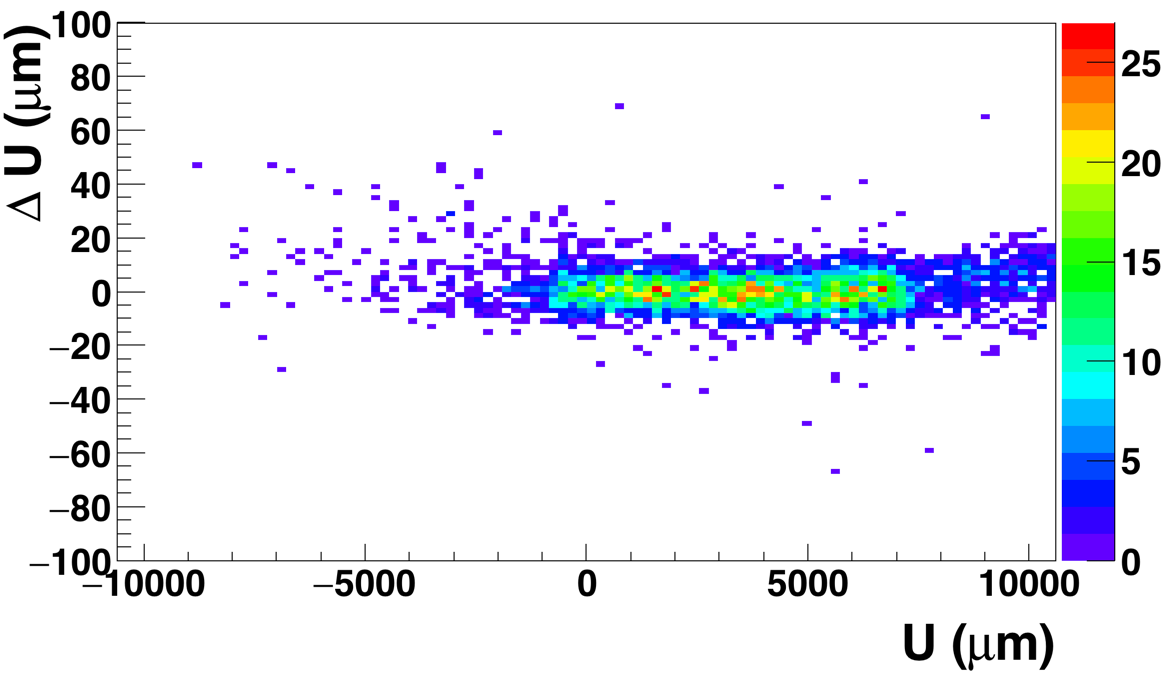
\includegraphics[width = 1.2\textwidth]{Pictures/deformation/deltaUU_8_corrected1.png}
          \caption{}
          \label{fig:scatterDUU_corrected_front}
        \end{subfigure}
        \hfill
        \begin{subfigure}[t]{0.45\textwidth}
          \centering
          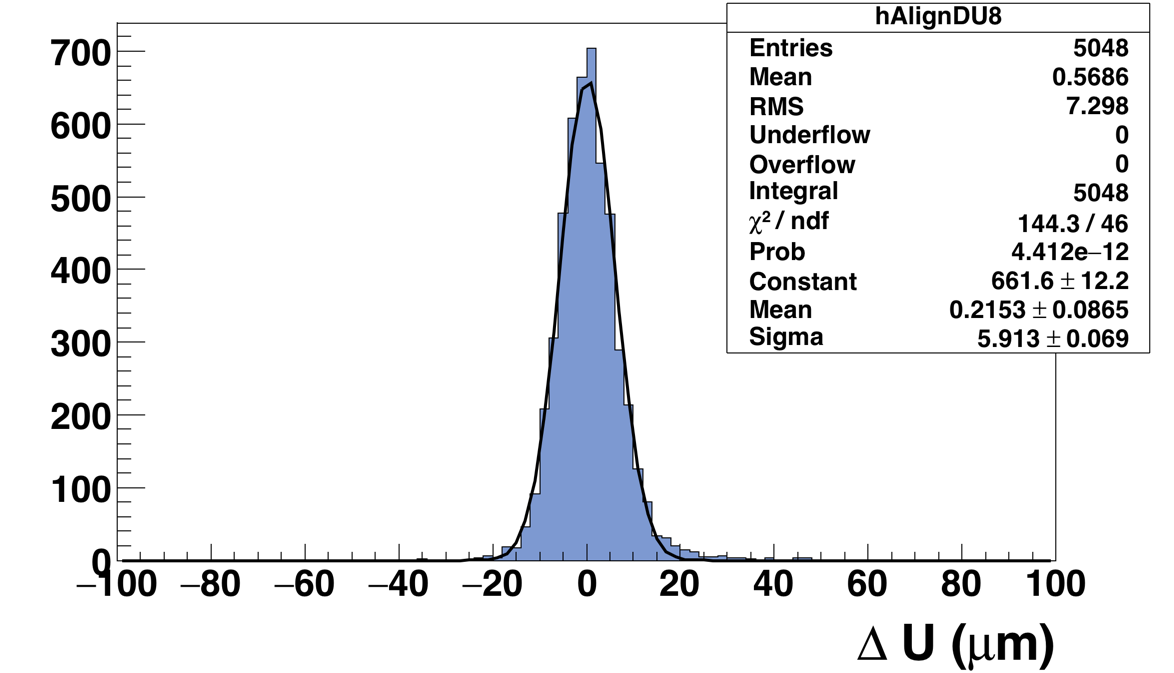
\includegraphics[width = 1.2\textwidth]{Pictures/deformation/deltaU_8_corrected1.png}
          \caption{}
          \label{fig:residualU_corrected}
        \end{subfigure}
        \caption{Results of the alignment after applying the Legendre polynomials correction and tacking into account the angle of the incoming particles for the front sensor: \ref{fig:scatterDUU_corrected_front} $\Delta u=f(u_{hit})$ and \ref{fig:residualU_corrected} distribution of the residuals.}
        \label{fig:alignmnetCorrected}

      \end{figure}

      \begin{figure}[!h]
        \centering
        \begin{subfigure}[t]{0.45\textwidth}
        \centering
          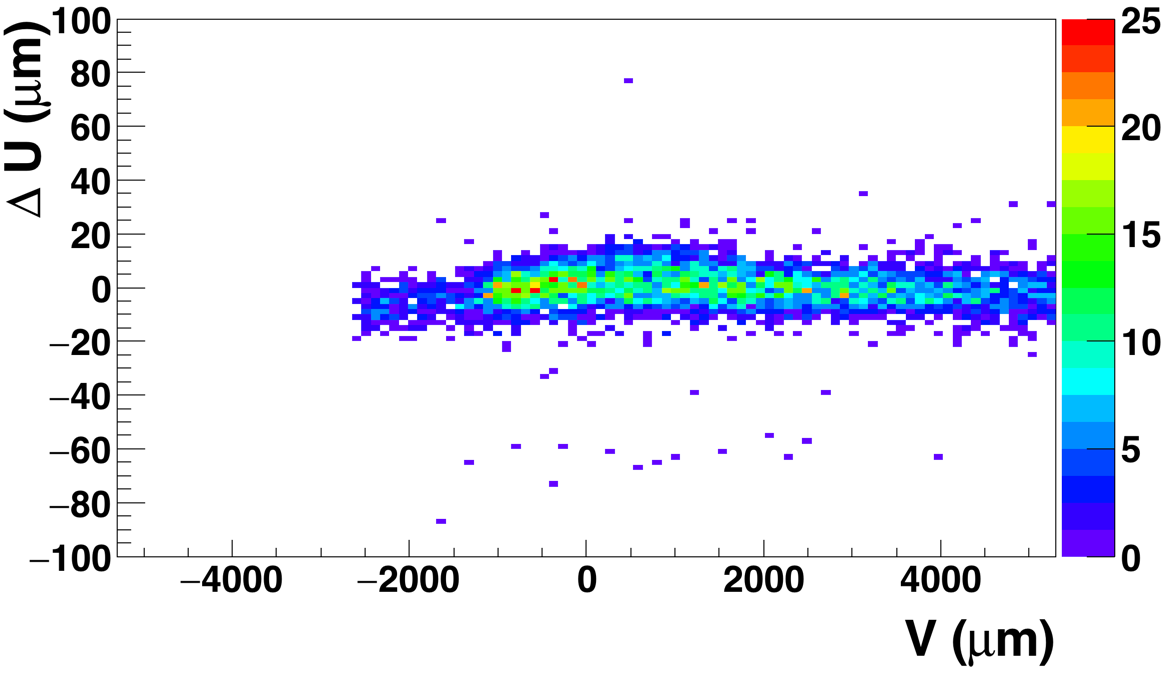
\includegraphics[width = 1.2\textwidth]{Pictures/deformation/deltaUV_6_corrected1.png}
          \caption{}
          \label{fig:scatterDUV_corrected_back}
        \end{subfigure}
        \hfill
        \begin{subfigure}[t]{0.45\textwidth}
          \centering
          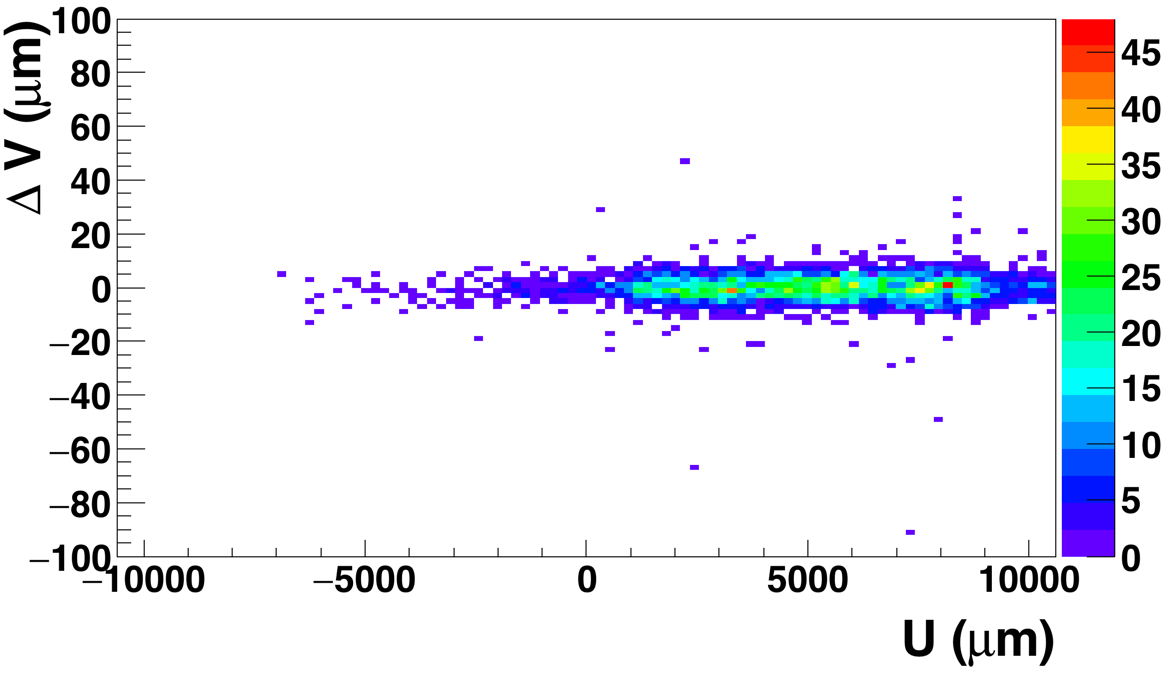
\includegraphics[width = 1.2\textwidth]{Pictures/deformation/deltaVU_6_corrected1.png}
          \caption{}
          \label{fig:scatterDVU_corrected_back}
        \end{subfigure}

        \begin{subfigure}[t]{0.45\textwidth}
          \centering
          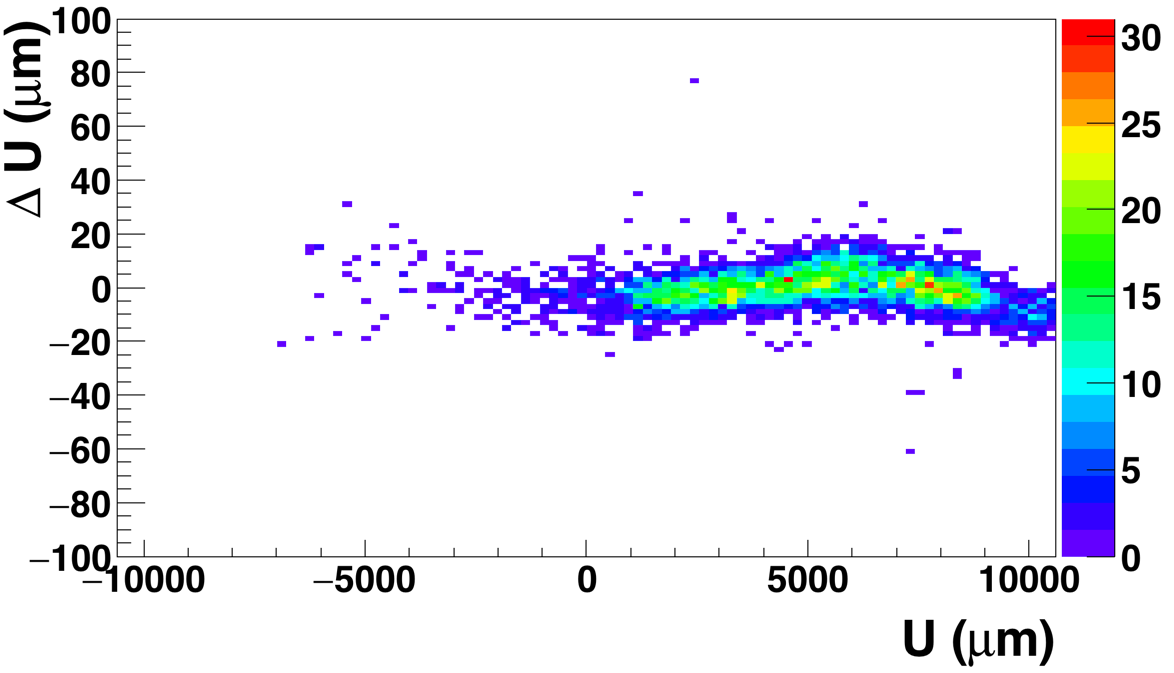
\includegraphics[width = 1.2\textwidth]{Pictures/deformation/deltaUU_6_corrected1.png}
          \caption{}
          \label{fig:scatterDUU_corrected_back}
        \end{subfigure}
        \hfill
        \begin{subfigure}[t]{0.45\textwidth}
          \centering
          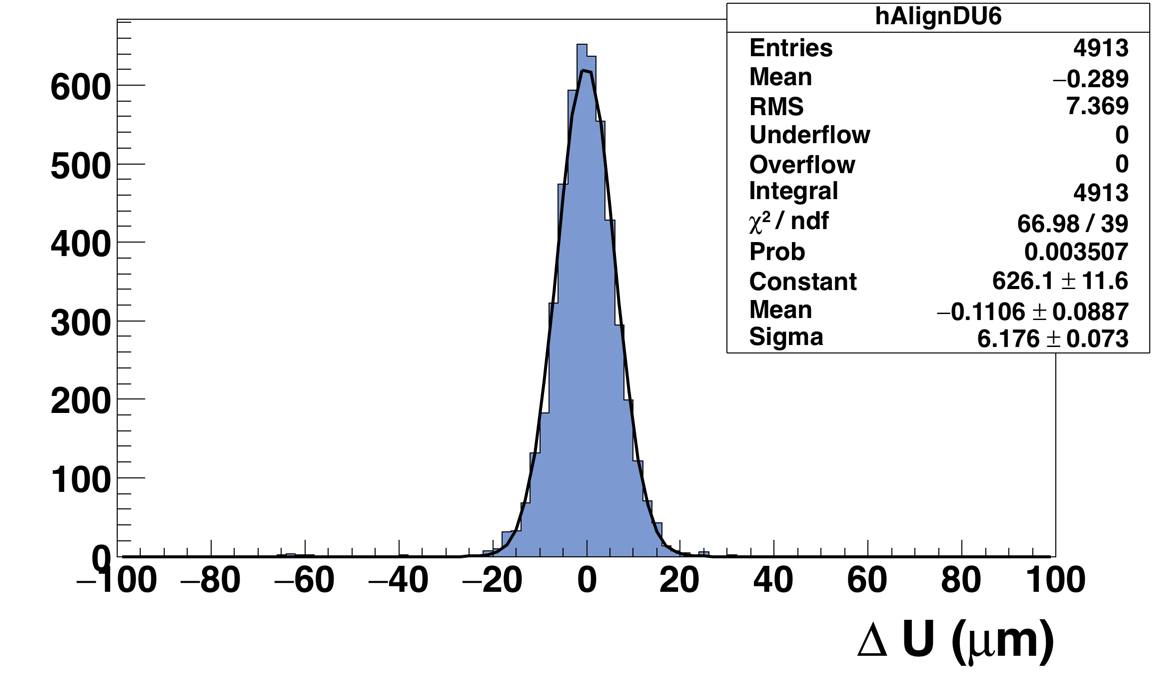
\includegraphics[width = 1.2\textwidth]{Pictures/deformation/deltaU_6_corrected1.png}
          \caption{}
          \label{fig:residualU_corrected_back}
        \end{subfigure}
        \caption{Results of the alignment after applying the Legendre polynomials correction and tacking into account the angle of the incoming particles for the back sensor: \ref{fig:scatterDUU_corrected_back} $\Delta u=f(u_{hit})$ and \ref{fig:residualU_corrected_back} distribution of the residuals.}
        \label{fig:alignmnetCorrected_back}

      \end{figure}

      This method was applied for different angles and the results are summarised in table~\ref{tab:correctionOfDeformation}. 
      The correction based on Legendre polynomials shows good results for the 28 degrees angle with a pointing resolution of 4.6 $\mu\text{m}$.
      Although for larger angles the precision is not expecting to reach the normal value, the results obtained are less positive.
      For the large angle (60 degrees), the position of the \gls{DUT} on the outside of the telescope arms does not provide a good telescope resolution ($\sigma_{tel} = 18.8 \text{ }\mu\text{m}$).
      The pointing resolution achieved for the front and back planes are respectively 10.8 $\mu\text{m}$ and 17.7 $\mu\text{m}$.
      The sensitivity of the reconstruction to large tracks angle, as well as a unadapted telescope configuration impact severely the spatial resolution of the sensors.

      \begin{table}[!h]
        \centering
        \begin{tabular}{c c c c c}
          \hline %----------------------------------------------------------------------------------------------------------------
          %Run Number  &  Plane Number &  Fan speed (m/s)   & Tilted angle  &   $\sigma_{U}^{Def}$ ($\mu m$) &   $\sigma_{U}^{Cor}$ ($\mu m$) & $\sigma_{U}^{DUT}$ ($\mu m$)\\
          %Side &  Tilted angle  &   $\sigma_{U}^{Def}$ ($\mu m$) &   $\sigma_{U}^{Cor}$ ($\mu m$) & $\sigma_{U}^{DUT}$ ($\mu m$)\\
          Side &  Tilted angle  &   $\sigma_{U}^{Def}$ ($\mu m$) &   $\sigma_{U}^{Cor}$ ($\mu m$) & Improvement \\
          \hline %----------------------------------------------------------------------------------------------------------------
          \hline %----------------------------------------------------------------------------------------------------------------
          %Front   & 3         &      28       &      9.586 &      5.568                       &    5.115           \\
          %Back    & 3         &      28       &      6.507 &      5.533                       &    5.077           \\
          %\hline %----------------------------------------------------------------------------------------------------------------
          %Front &      28       & $ 8.8 \ \pm \ 0.1 $ & $ 4.8 \ \pm \ 0.1 $ &    $45.5 \ \%$  \\
          %Back  &      28       & $ 5.6 \ \pm \ 0.1 $ & $ 4.5 \ \pm \ 0.1 $ &    $19.6 \ \%$ \\
          Front &      28       & $ 9.0 \ \pm \ 0.1 $ & $ 4.9 \ \pm \ 0.1 $ &    $46.6 \ \%$  \tabularnewline
          Back  &      28       & $ 5.7 \ \pm \ 0.1 $ & $ 4.7 \ \pm \ 0.1 $ &    $17.5 \ \%$  \tabularnewline
          %\hline %----------------------------------------------------------------------------------------------------------------
          \hline %----------------------------------------------------------------------------------------------------------------
          Front &      36       & $ 14.1 \ \pm \ 0.1 $ & $ 6.1 \ \pm \ 0.1 $ &    $56.0 \ \%$ \tabularnewline
          Back  &      36       & $ 6.8 \ \pm \ 0.1 $ & $ 5.9 \ \pm \ 0.1 $ &    $13.2 \ \%$  \tabularnewline
          %\hline %----------------------------------------------------------------------------------------------------------------
          \hline %----------------------------------------------------------------------------------------------------------------
          Front &      60       & $ 41.2 \ \pm \ 0.15$ & $25.8 \ \pm \ 0.2$  &    $37.4 \ \%$ \tabularnewline
          Back  &      60       & $ 23.3 \ \pm \ 0.13$ & $21.7 \ \pm \ 0.1$  &    $6.8 \ \%$  \tabularnewline
          \hline %----------------------------------------------------------------------------------------------------------------
        \end{tabular}
        \caption{Alignment results for different angles before and after using the correction based on Legendre polynomials.}
        \label{tab:correctionOfDeformation}
      \end{table}

      A hypothesis on the deformation of the origin might come from heating or the cooling system that induces vibration.
      Although few runs were performed with a different air flow speed, the impact of the cooling system and the heat was not planned for this test beam.
      Thus, the results are not relevant enough to conclude for any vibration or the heat that tends to deform more the surface.
    
  \section{Benefits of double-sided measurement}
  
  As two modules are sharing the same mechanical structure, the information provided by each side can be combined together.
  A mini-vector is created by connecting two hits on each side of the ladder for the same event.
  This combination gives access to a new information compared to a single sensor: the angular resolution.

    \subsection{Spatial resolution with mini-vectors}

    To study the benefits of the mini-vector, a virtual intermediate plane is defined at the center of the ladder.
    The two hits of each side of the \gls{DUT} are connected to form a mini-vector and the intersection of this vector to the intermediate plane is determined.
    The intersection of the extrapolated track to the intermediate plane is also performed and the distance between the position of the track and the position of the mini is then measured.

    \begin{figure}[!h]
      \centering
      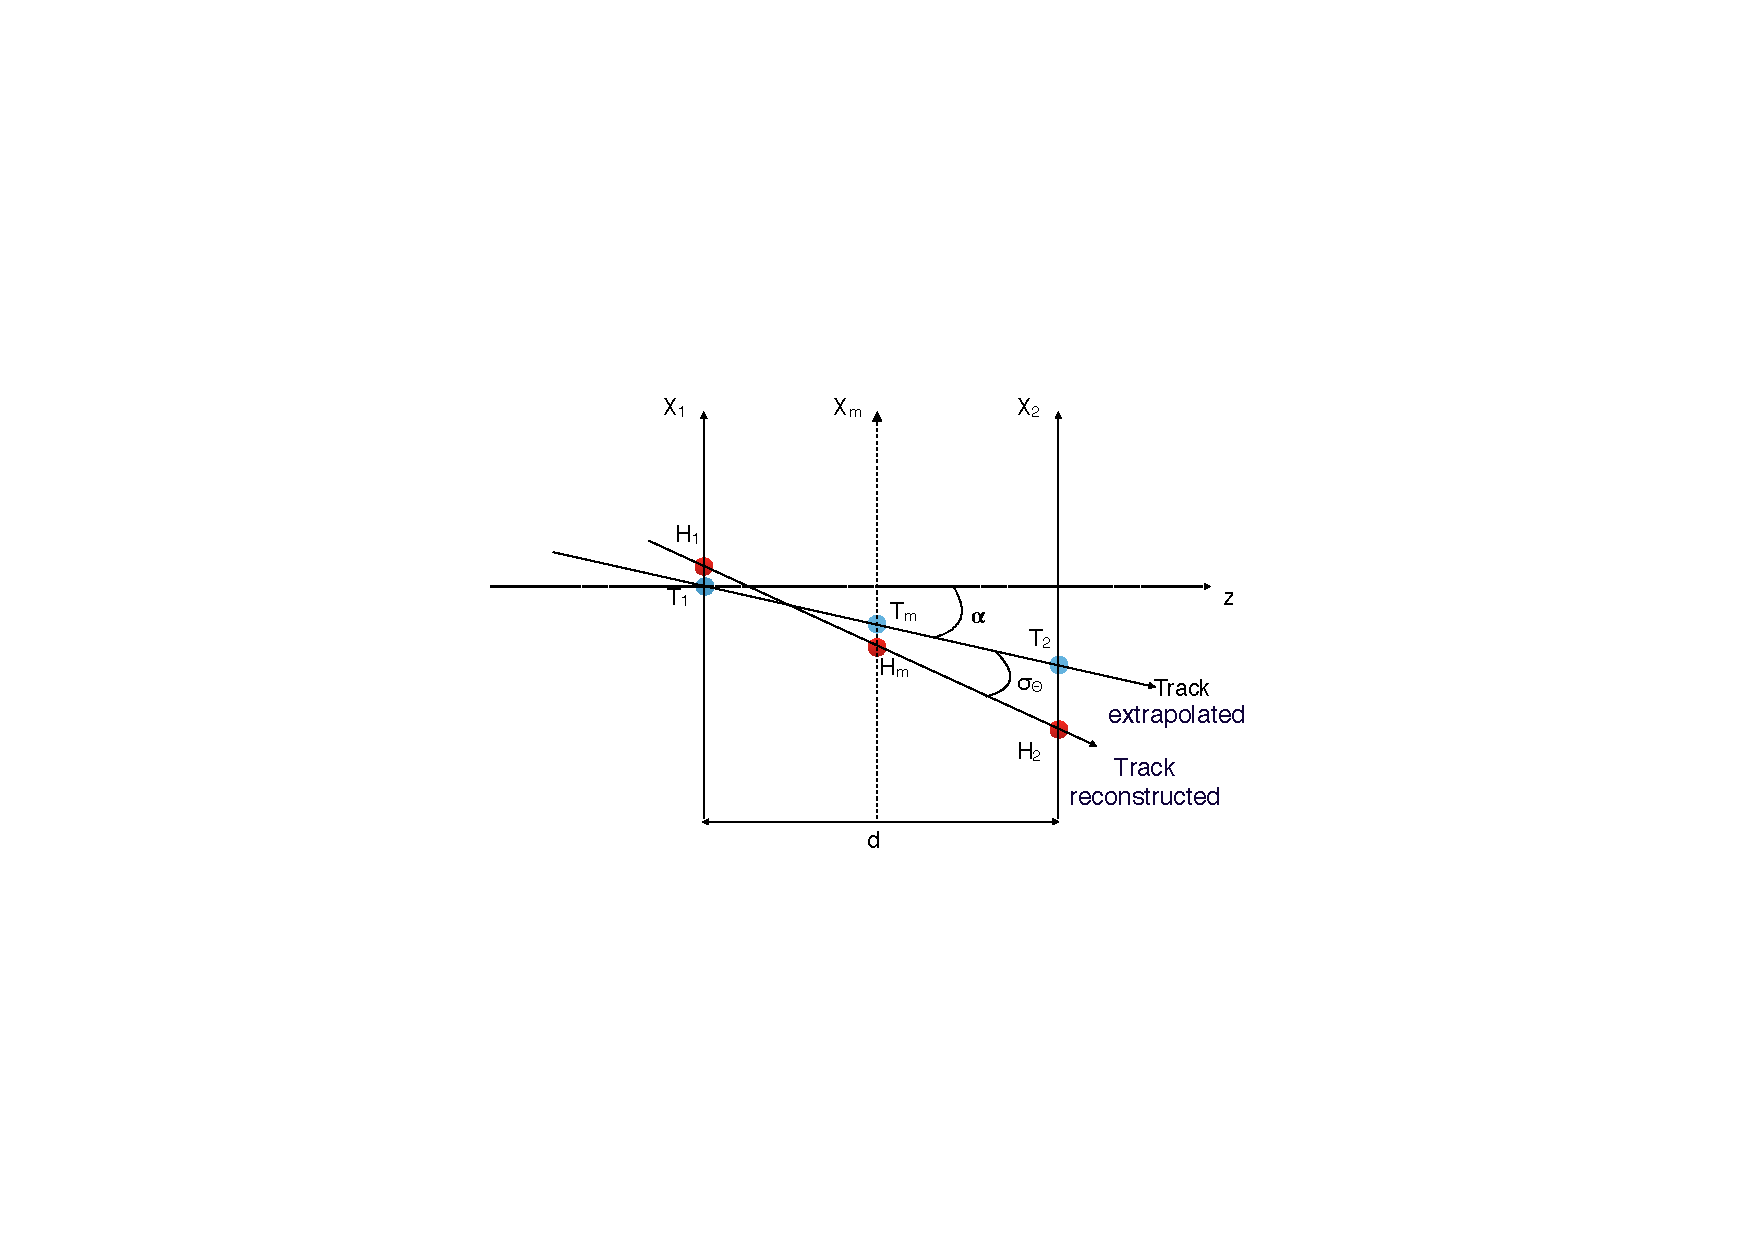
\includegraphics[width=0.7\textwidth]{Pictures/deformation/mini_vectors.pdf}
      \caption{Principle of the mini-vector. The two hits (in red) on the planes $x_1$ and $x_2$ are connected and the intersection on virtual intermediate plane $x_m$ is then determined. The blue points represents the track extrapolated through the DUT. }
      \label{fig:MV}
    \end{figure}

    A theoretical estimation of the spatial resolution for the mini-vector can be done thanks to the formula above:

    \begin{equation}
      \sigma_m^2 = \frac{\sigma_{front}^2 + \sigma_{back}^2}{(d_{front} - d_{back})^2} \cdot d_{m}^2 + \sigma_{tel}^2
      \label{eq:resolutionMV}
    \end{equation}

    Where $\sigma_m$ is the resolution on the intermediate plane, $\sigma_{front}$ and $\sigma_{back}$ are the resolution of the two sides of the \gls{DUT}, $\sigma_{tel}$ the resolution of the telescope and $(d_{front} - d_{back})$ the distance between the front and back planes and $d_{m}^2$ the position of the intermediate plane.
    For the plume ladder, the \gls{SiC} as a thickness of 2 mm and the intermediate plane is located in the middle, the equation~\ref{eq:resolutionMV} can be rewritten:

    \begin{equation}
      \sigma_m^2 = \frac{\sigma_{front}^2 + \sigma_{back}^2}{4} + \sigma_{tel}^2
    \end{equation}

    Thus, if the resolution on both side of the telescope are similar with $\sigma_{front} = \sigma_{back} = \sigma$, the resolution of the mini-vector $\sigma_{res}$ is then:

    \begin{equation}
      \sigma_{res} = \frac{\sigma}{\sqrt{2}}
    \end{equation}

    \begin{figure}[!h]
      \centering
      \begin{subfigure}[t]{0.45\textwidth}
        \centering
        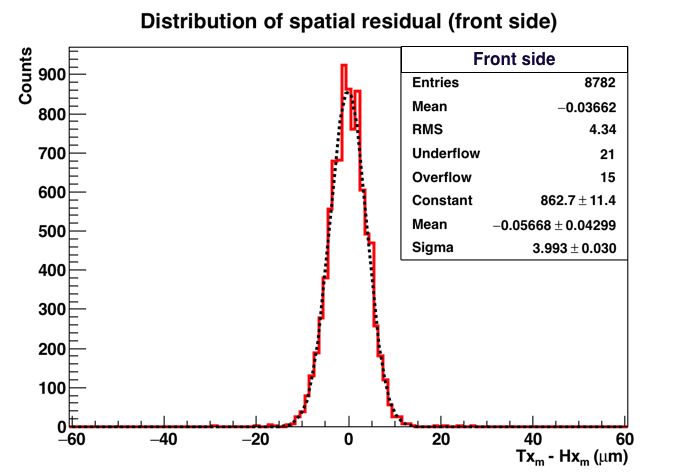
\includegraphics[width = 1.2\textwidth]{Pictures/deformation/hxtxFront_226056.png}
      \end{subfigure}
      \quad
       %add desired spacing between images, e. g. ~, \quad, \qquad, \hfill etc. 
        %(or a blank line to force the subfigure onto a new line)
      \begin{subfigure}[t]{0.45\textwidth}
        \centering
        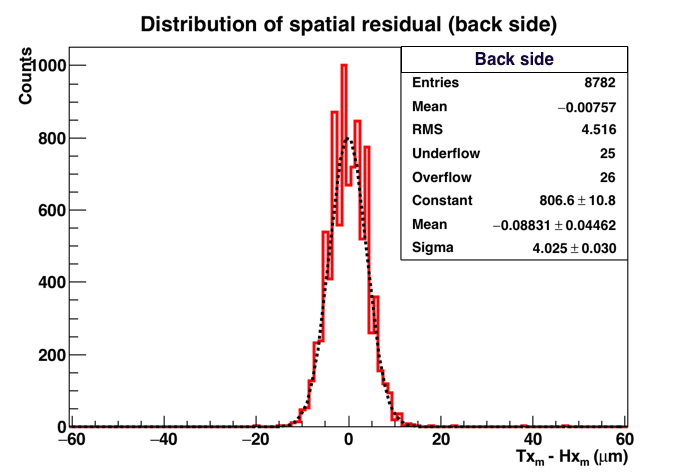
\includegraphics[width = 1.2\textwidth]{Pictures/deformation/hxtxBack_226056.png}
      \end{subfigure}
      \caption{Residual distribution for both side of the ladder in the $u$-direction}
      \label{fig:residualFrontBackLadder}
    \end{figure}

    \begin{figure}[!h]
      \centering
      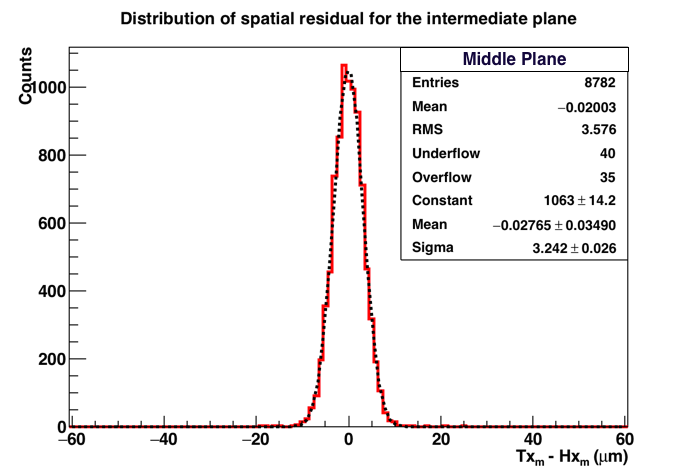
\includegraphics[width = 0.7\textwidth]{Pictures/deformation/hDiffPosX_226056.png}
      \caption{Residual distribution of the mini-vector measured on the intermediate plane.}
      \label{fig:residualMV}
    \end{figure}

    For a run in normal incidence, the spatial resolution measured on each side is $\sigma_{front} \simeq \sigma_{back} \simeq 4 \text{ }\mu\text{m}$, according to figure~\ref{fig:residualFrontBackLadder}.
    The resolution of the mini-vector should be then $\sigma_{res} \simeq 2.8 \text{ }\mu\text{m}$.
    The measurement of the residual for the mini-vector displayed on figure~\ref{fig:residualMV} gives a residual of 3.2 $\mu\text{m}$.
    Taking into account the resolution of the telescope, the spatial resolution achieved by the mini-vector is $\sigma_{res} \simeq 2.9 \text{ }\mu\text{m}$.



   \subsection{Angular resolution}

   The mini-vectors give an access to new information not provided by a single sensor, the angular resolution.
   The direction of the track can be compared to the direction of the mini-vector.
   The estimation of the angular resolution is given by:

   \begin{equation}
     \sigma_{theta} = \frac{\sqrt{\sigma_{front}^2 + \sigma_{back}^2}}{d}
     \label{eq:angularResolution}
   \end{equation}

   With $\sigma_{front}$ and $\sigma_{back}$ the spatial resolution on each side of the \gls{DUT} in microns and d the distance between the two sides in microns.
   The spatial resolution here is $\sigma \simeq 3.6 \text{ }\mu\text{m}$ and the distance between the two planes 2000 microns.
   The angular resolution estimated is then $\sigma_{\theta} = 0.146^{\degree}$.  
   
   \begin{figure}[!h]
     \centering
     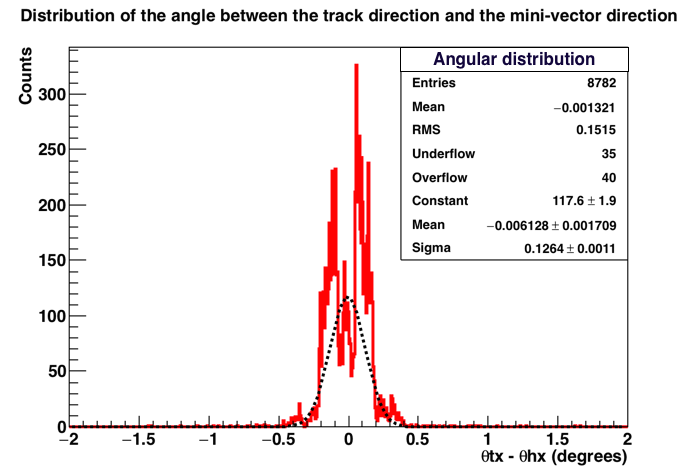
\includegraphics[width = 0.7\textwidth]{Pictures/deformation/hDiffAngleX_226056.png}
     \caption{Distribution of the angle between the tracks direction and the mini-vectors direction.}
     \label{fig:angRes}
   \end{figure}

   Figure~\ref{fig:angRes} depicts the distribution of the angle between the tracks direction and the mini-vectors direction.
   As it can be seen, several peaks are present and the distribution can't be extrapolated by a Gaussian fit.
   The sensors have a binary output and the hit position is determined by the centre-of-gravity of the clusters.
   If the cluster is only one pixel, the centre-of-gravity will be in the middle of the pixel, but if the clusters contain more pixels, this centre-of-gravity will be displaced.
   Moreover, they are some deviations in the distance between the hit projected to one side to the real hit position on this side.
   Figure~\ref{fig:clusterSize} represents the minimum distance between one cluster on one side to the cluster on the other side.
   
   \begin{figure}[!h]
     \centering
      \begin{subfigure}[t]{0.45\textwidth}
         \centering
         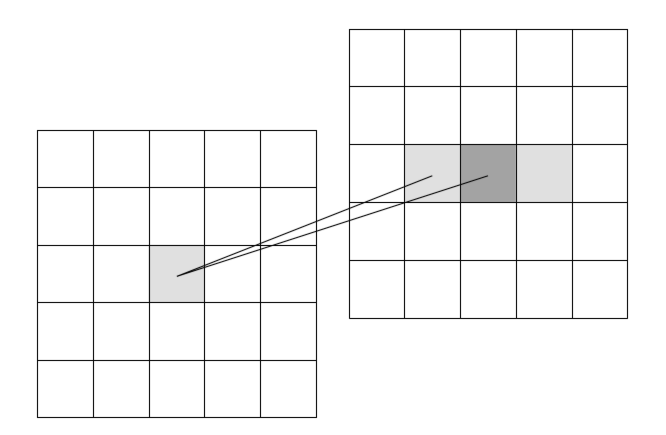
\includegraphics[width = \textwidth]{Pictures/deformation/cluster_1x1.png}
         \caption{One pixel per cluster.}
      \end{subfigure}
      \quad
       %add desired spacing between images, e. g. ~, \quad, \qquad, \hfill etc. 
        %(or a blank line to force the subfigure onto a new line)
      \begin{subfigure}[t]{0.45\textwidth}
        \centering
        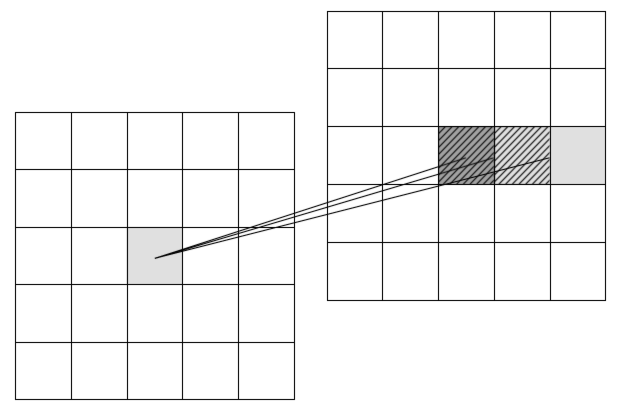
\includegraphics[width = \textwidth]{Pictures/deformation/cluster_1x2.png}
        \caption{$1 \times 2$ pixels per cluster.}
      \end{subfigure}
      
      \begin{subfigure}[t]{0.45\textwidth}
        \centering
        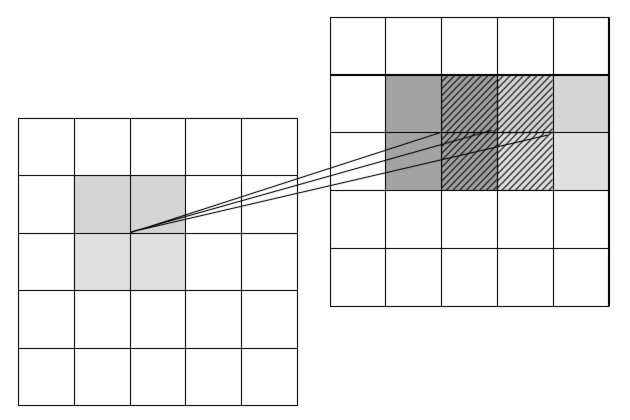
\includegraphics[width = \textwidth]{Pictures/deformation/cluster_2x2.png}
        \caption{$2 \times 2$ pixels per cluster.}
      \end{subfigure}
      \quad
      \begin{subfigure}[t]{0.45\textwidth}
        \centering
        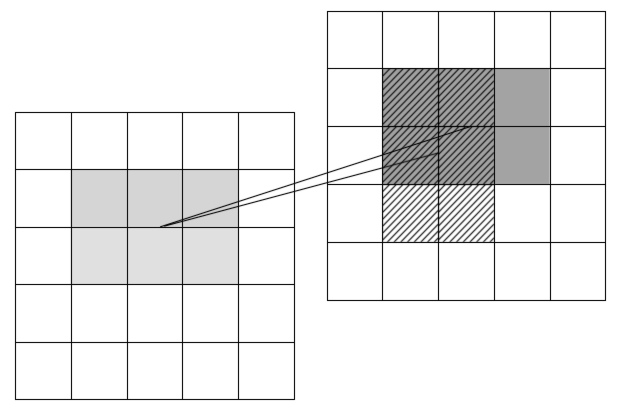
\includegraphics[width = \textwidth]{Pictures/deformation/cluster_3x3.png}
        \caption{$3 \times 3$ pixels per cluster.}
      \end{subfigure}
      \caption{Minimum distance between the cluster projected on one side to the position of the cluster of this side.}
      \label{fig:clusterSize}
   \end{figure}

   Hence, for one pixel clusters, the displacement between the two pixels is the pitch $p = 18.4 \text{ }\mu\text{m}$ and the angle between the two minimal hit position is then $\theta \sim 0.52^{\degree}$.
   A selection of the events where only clusters of 1 pixel are considered is shown on figure~\ref{fig:angRes1x1}.
   The two peaks have a spacing close to $0.5^{\degree}$.
   For clusters of $1 \times 2$ or $2 \times 2$ pixels, the distance between the two hit positions reconstructed via centre-of-gravity is half the pitch.
   Hence, the peaks are two times closer with a spacing of nearly $0.25^{\degree}$, as seen on figures~\ref{fig:angRes2x1} and~\ref{fig:angRes2x2}.
   Nevertheless, for larger cluster sizes the angular distribution has only one peak around $0^{\degree}$.


   \begin{figure}[!h]
     \centering
      \begin{subfigure}[t]{0.45\textwidth}
         \centering
         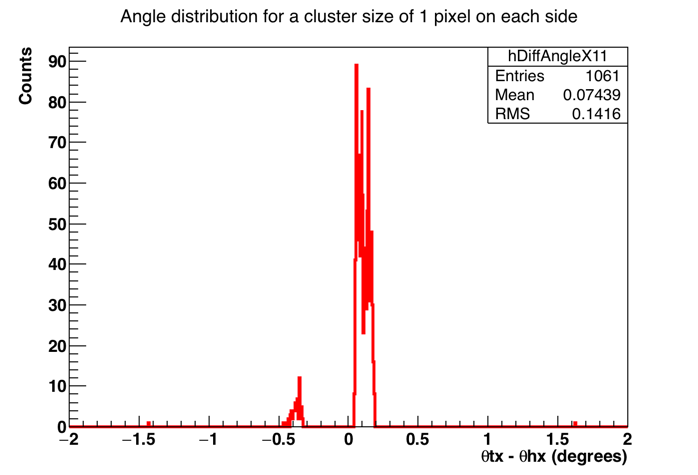
\includegraphics[width = \textwidth]{Pictures/deformation/hDiffAngleX11_226056.png}
         \caption{One pixel per cluster.}
         \label{fig:angRes1x1}
      \end{subfigure}
      \quad
       %add desired spacing between images, e. g. ~, \quad, \qquad, \hfill etc. 
        %(or a blank line to force the subfigure onto a new line)
      \begin{subfigure}[t]{0.45\textwidth}
        \centering
        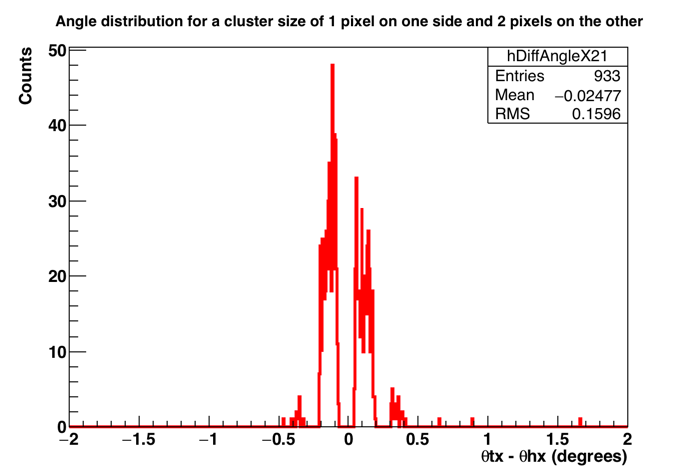
\includegraphics[width = \textwidth]{Pictures/deformation/hDiffAngleX21_226056.png}
        \caption{$2 \times 1$ pixels per cluster.}
        \label{fig:angRes2x1}
      \end{subfigure}
      
      \begin{subfigure}[t]{0.45\textwidth}
        \centering
        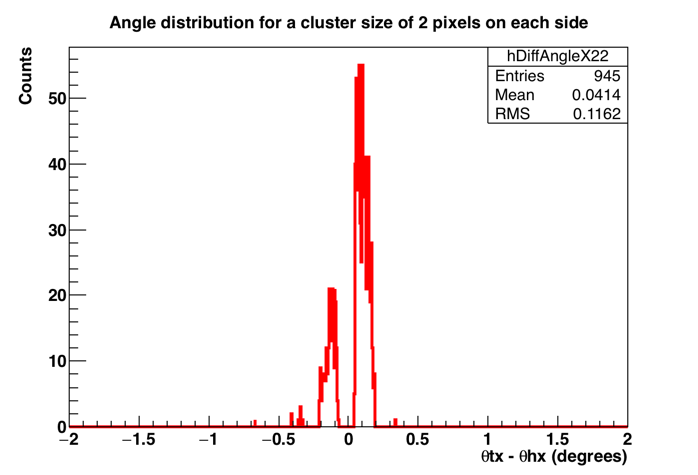
\includegraphics[width = \textwidth]{Pictures/deformation/hDiffAngleX22_226056.png}
        \caption{$2 \times 2$ pixels per cluster.}
        \label{fig:angRes2x2}
      \end{subfigure}
      \quad
      \begin{subfigure}[t]{0.45\textwidth}
        \centering
        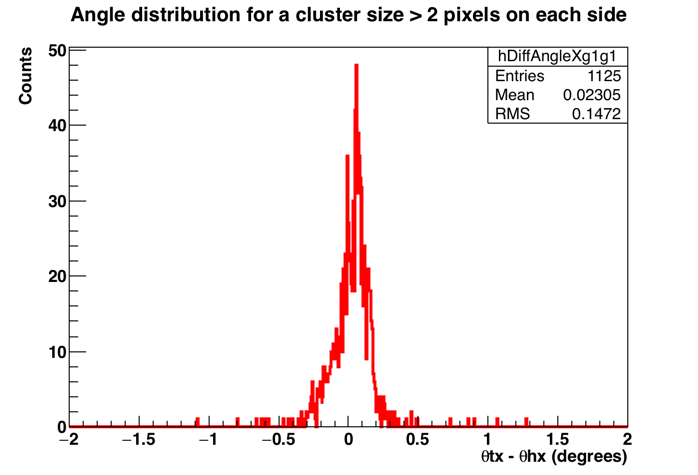
\includegraphics[width = \textwidth]{Pictures/deformation/hDiffAngleXg1g1_226056.png}
        \caption{Clusters bigger than $2 \times 2$ pixels.}
      \end{subfigure}
      \caption{Minimum distance between the cluster projected on one side to the position of the cluster of this side.}
      \label{fig:anglResDecomposed}
   \end{figure}
   

  \section{Conclusions}

  Along this chapter, the test beam campaign done in November 2011 at CERN was discussed. 
  The results were focused on the alignment procedure, as well as the performances of the ladder in normal and tilted positions.
  The runs in tilted position were challenging to align due to some deviations between the track-hit residual and the actual hit position on the plane.
  This has the effect of increasing the spatial residual measured.
  A higher pointing resolution is expected for bending tracks but in a smaller proportion.
  An algorithm using Legendre polynomials to describe the sensor's shape was discussed.
  The results obtained for small angles are close to the value expected for a single MIMOSA-26 sensor in normal incidence. 
  Nevertheless, the pointing resolution depends strongly on the incidence angle.
  For $36^{\degree}$ and higher, the correction is less efficient to achieve the normal performances.
  It might also be possible that the heating is increasing the deformation and that the cooling system could induce some vibrations which induce some deformation too.
  Nevertheless, the results obtained here for different air flow speed can not lead to a conclusion on a possible impact of the cooling system.

  The second part of this chapter was talking about the benefits of double-sided measurements.
  For normal incidence, the pointing resolution of the mini-vector, which is the combination of the pointing resolution on each side,  is better than the spatial resolution of a single sensor.
  Moreover, the mini-vectors give access to another information: the angular resolution.
  Due to the binary output and the centre-of-gravity hit position reconstruction, multiple peaks are visible and a simple Gaussian fit can not be used. 
  The same work has to be done with ladder titled with respect to the beam to study the impact of the deformation on the mini-vectors.

  The first results obtained are encouraging the mechanical structure.
  Nevertheless, the material budget of the ladder is estimated theoretically.
  The next chapter will introduce a test beam performed at DESY in 2016 and will specifically talk about the measurement of the radiation length for a PLUME-V1 prototype.

